\documentclass[language=en,11pt]{aghdpl}  % praca w języku angielskim

%---------------------------------------------------------------------------

\author{Kacper Motyka}
\shortauthor{K. Motyka}

\titlePL{Analiza porównawcza wpływu technik augmentacji obrazu na wydajność sieci neuronowych w zadaniach klasyfikacji obrazu}
\titleEN{Comparative Analysis of the Image Data Augmentation Techniques Impact on Neural Network Performance in Image Classification Tasks}


\shorttitlePL{Przygotowanie pracy dyplomowej w~systemie \LaTeX} 
\shorttitleEN{Analysis of the Image Data Augmentation}


% Dopuszczalne wartości[1,2]:
% * "Projekt dyplomowy" - na koniec studiów I stopnia
% * "Praca dyplomowa" - na koniec studiów II stopnia
% [1] Zasady dyplomowania w roku akademickim 2020/2021 (Decyzja Dziekana WEAIiIB nr 16/2020 z dnia 9 grudnia 2020 roku)
% [2] Załącznik nr 1a) do Decyzji nr 16/2020 Dziekana Wydziału EAIiIB z dnia 09 grudnia 2020 r.
\thesistype{Master Thesis}

\supervisor{Krzysztof Kluza, PhD}


\degreeprogramme{Computer Science and Intelligent Systems}

\date{2024}

%\department{Katedra Informatyki Stosowanej}
%\department{Department of Applied Computer Science}

\faculty{Faculty of Electrical Engineering, Automatics, Computer Science and Biomedical Engineering}


\begin{document}

	\titlepages
	\RedefinePlainStyle
	
	\setcounter{tocdepth}{2}
	\tableofcontents
	\clearpage
	\chapter{Introduction}
\label{cha:Introduction}

%---------------------------------------------------------------------------

\section{Background and Motivation}
\label{sec:background}

The field of deep learning, particularly in image classification tasks, has seen remarkable advancements in recent years. Neural networks have become the cornerstone of image recognition, enabling applications ranging from autonomous vehicles to medical diagnostics.

Despite these advancements, the performance of neural networks, particularly in image classification tasks, significantly depends on the quality and volume of the training data. High-quality, diverse datasets are crucial for training robust models capable of understanding and categorizing images accurately. However, in many real-world scenarios, the acquisition of a large, well-labeled dataset is resource-intensive and sometimes, practically impossible. 

This limitation underscores the critical importance of data augmentation, a method to artificially enhance the volume and diversity of training datasets, which has become a key technique for improving the performance of neural networks without the need for additional raw data. Data augmentation techniques can simulate a wider range of scenarios and conditions, thereby enriching the training set and improving the model's generalization capabilities.

Traditional augmentation techniques, such as geometric transformations and color space adjustments, have provided foundational improvements in model training. With the arrival of more sophisticated methods, including CutMix, MixUp, and synthetic data generation through Generative Adversarial Networks (GANs), the potential for achieving even greater improvements in network performance has expanded. 

This thesis conducts a comparative analysis of these augmentation techniques to identify their impact on image classification outcomes. The study seeks to highlight the effectiveness of various augmentation strategies, thereby providing insights that could optimize the training of neural networks.

%---------------------------------------------------------------------------

\section{Objectives of the Study}
\label{sec:objectives}

The main objective of the study is to compare classical and advanced image data augmentation techniques, including but not limited to CutMix, MixUp, and GAN-generated data, to evaluate their impact on neural network performance.

Taking into account  that the effectiveness of data augmentation techniques may vary based on dataset characteristics, to obtain more general results, this study aims to compare a variety of datasets, including:
\begin{enumerate}
    \item A \textbf{standard}, well-balanced dataset.
    \item A dataset with a \textbf{limited number of samples} per category, simulating a one-shot learning scenario to assess augmentation techniques in data-scarce situations.
    \item A \textbf{domain-specific} dataset to explore the effectiveness of augmentation methods distinct to specialized fields' characteristic challenges and requirements.
\end{enumerate}

Based on the findings, the goal is to offer insights and recommendations on selecting and implementing data augmentation strategies tailored to the unique needs of different image classification tasks and dataset characteristics.

%---------------------------------------------------------------------------

\section{Limitations}
\label{sec:scope}

The study is limited to \textbf{selected datasets} and \textbf{neural network architectures}. While the research attempts to cover a broad range of augmentation methods, it acknowledges that the rapidly evolving landscape of deep learning might yield \textbf{new techniques} beyond the scope of this thesis. Additionally, the experimental design is tailored to assess augmentation impacts under specific conditions and configurations, which may not encapsulate \textbf{all potential application scenarios}. The findings are intended to provide valuable insights and recommendations, although with the understanding that results might vary with different datasets, neural network architectures, or task-specific requirements.

\section{Thesis Structure}

The thesis begins with an introduction, providing an overview of the motivation, objectives, and limitations of the study. This chapter sets the context for the entire research.

Following the introduction, the second chapter presents the fundamental concepts underlying neural networks. It covers deep neural networks, convolutional neural networks, generative adversarial networks, and transfer learning, providing the necessary theoretical background for the following analysis.

The third chapter focuses on data augmentation techniques, which are the main topic of the thesis. This chapter presents a justification for the use of data augmentation, explores both traditional and advanced methods, discusses the application of GANs in data augmentation, and considers domain-specific techniques.

In the fourth chapter, the methodology is detailed. This includes descriptions of the datasets used, data preprocessing steps, convolutional neural network architectures employed, and the evaluation metrics selected for assessing the impact of data augmentation techniques on model performance.

The fifth chapter describes the experiments and presents the results. It details the implementation specifics concerning GANs and CNNs training, and the outcomes of applying various data augmentation techniques to CNN performance. This chapter also interprets the results and discusses their broader implications.

Finally, the sixth chapter concludes the thesis by summarizing the key insights and contributions of the study and suggesting directions for future research in the area.
	\chapter{Fundamental Concepts Underlying Neural Networks}
\label{cha:fundanemtalConcepts}

%---------------------------------------------------------------------------

This thesis begins by introducing theory related to neural networks which derive their name from the networks of biological neurons present in our brains. However, although airplanes draw inspiration from birds, they do not need to flap their wings. Similarly, even though neural networks are derived from biological neurons, they became quite different from their biological equivalent, so many scientists believe that this analogy should be abandoned. The reason is to avoid constraining our creativity to structures that can only exist in nature and to open up the potential for more innovative designs that exceed natural limitations~\cite{UMzUSLiTF}.

\section{Perceptrons}

Neural networks consist of \textit{perceptrons} (artificial neurons) which are interconnected to form a more complex structure. To fully understand how neural networks work, it is essential to explain the function of a single perceptron first.

In 1957, Frank Rosenblatt proposed the perceptron, which is the simplest form of an artificial neural network. It is based on an artificial neuron known as a \textit{Threshold Logic Unit} or \textit{TLU}~\cite{UMzUSLiTF}.

\begin{figure}[!htb]
    \centering
    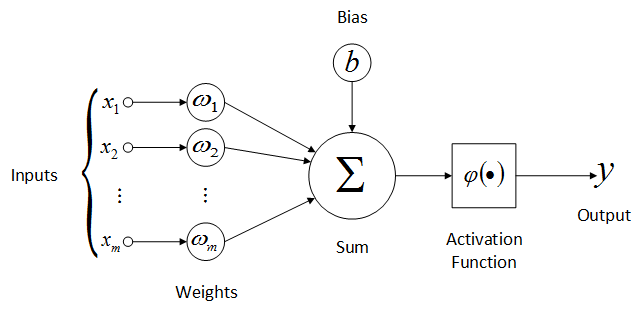
\includegraphics[scale=0.6]{Images/perceprton-model.png}
    \caption{Perceptron model~\cite{PerceptronModel}.}
    \label{fig:perceptronModel}
\end{figure}

The diagram in Figure \ref{fig:perceptronModel} illustrates the structure of a single perceptron, which consists of four essential elements: \textbf{inputs}, \textbf{weights and bias}, a \textbf{summation function}, and an \textbf{activation function}.

The functionality of a perceptron can be described as follows: the inputs and outputs are numerical values, and each connection has assigned a specific weight. The perceptron calculates the sum of the input values each multiplied by their respective weights and adds a bias term to this calculated sum:

\begin{equation}
z = b + \sum_{i=1}^{n} x_iw_i = x^Tw + b
\end{equation}

This weighted sum is then passed through an activation function, which determines the final output value of the perceptron:

\begin{equation}
y = \phi(z)
\end{equation}

A perceptron is composed of a single layer of \textit{TLU} units, with each \textit{TLU} connected to every input. Such a layer is referred to as a fully connected layer. Inputs are fed into artificial neurons, also known as the input layer, whose function is to forward all the received data. Moreover, it is worth mentioning that a perceptron can have more than one output, enabling it to classify samples into multiple categories, therefore functioning as a multi-output classifier~\cite{UMzUSLiTF}~.

Frank Rosenblatt's learning algorithm was inspired by Hebb's rule, which states that when a biological neuron frequently excites another nerve cell, the connection between these neurons becomes stronger. Siegrid Löwel summarized this concept with the phrase: "Cells that fire together, wire together," which loosely translates to "Cells that excite each other tend to connect more strongly." This means that the connection weight between two neurons tends to increase when they are activated at the same time.

Perceptrons use a variant of this rule during training, taking into account the error the network makes during outcome predictions. This means that connections that help reduce the error value are strengthened. More specifically, the perceptron processes one training example at a time and calculates predictions for each. For each output neuron responsible for an incorrect result, the weights of connections from all inputs contributing to the correct prediction are increased. 

The equation \ref{eq:weightsUpdate} represents the process of updating weights in perceptron learning:

\begin{equation}
    w_{i,j}^{k + 1} = w_{i,j}^k + \eta(y_j - \bar{y}_j)x_i
    \label{eq:weightsUpdate}
\end{equation}

where:
\begin{eqwhere}[2cm]
\item[$w_{i,j}$] is the weight of the connection between the i-th input and the j-th output neuron
\item[$x_i$] is the i-th input value of the current training example
\item[$\bar{y}_j$] is the output of the j-th output neuron for the current training example
\item[$y_j$] is the expected output of the j-th output neuron for the current training example
\item[$\eta$] is the learning rate
\item[$k$] is the step
\end{eqwhere}

It is worth noting that Rosenblatt proved that the learning algorithm will converge if the training samples are linearly separable. A concept was formalized in the perceptron convergence theorem~\cite{UMzUSLiTF}.

\section{Deep Neural Networks}

In their simplest form, perceptrons have several significant drawbacks. Marvin Minsky and Seymour Papert pointed out some of these limitations in their 1969 monograph, "Perceptrons"~\cite{PerceptronsBook}. For instance, the perceptron cannot solve trivial problems, such as the exclusive OR (XOR) classification task. However, researchers have discovered that many of these limitations can be overcome by creating multiple layers of perceptrons. 

A \textit{Multi-Layer Perceptron} (\textit{MLP}) consists of one input layer, at least one hidden layer of Threshold Logic Units (TLUs), and a final output layer. This architecture enables the MLP to tackle problems that a single-layer perceptron cannot, including the XOR problem.

\begin{figure}[!htb]
    \centering
    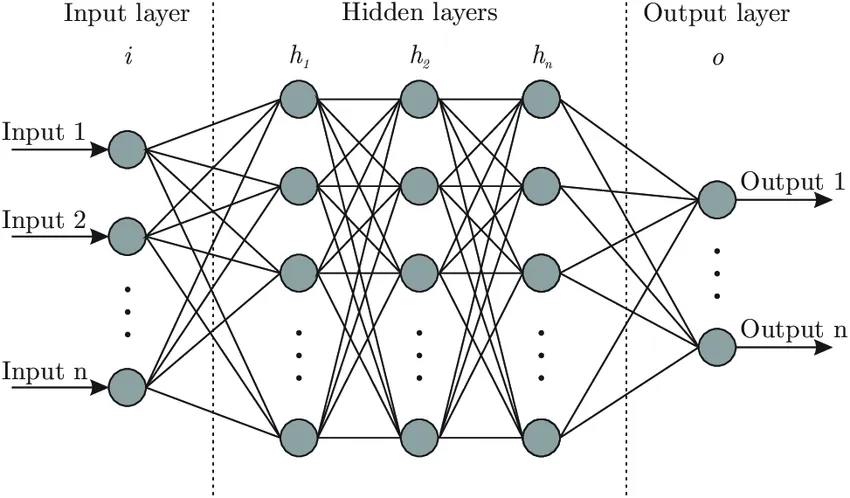
\includegraphics[scale=0.5]{Images/nn_model.jpg}
    \caption{Neural network model~\cite{NNModel}.}
    \label{fig:NNModel}
\end{figure}

An artificial neural network is called a \textit{Deep Neural Network (DNN)} if it contains multiple hidden layers. It is noteworthy that the term "deep" is quite relative - it can imply anything from a few to over a hundred hidden layers. Layers located close to the output layer are called upper layers, while those closer to the input layer are known as lower layers. Each layer includes a bias neuron and is fully connected to the subsequent layer.

For decades, scientists have been searching for an effective way to train deep neural networks. The breakthrough arrived in 1986 with the introduction of the \textbf{backpropagation algorithm} by David Rumelhart, Geoffrey Hinton, and Ronald Williams~\cite{UMzUSLiTF}.

The backpropagation algorithm leverages the gradient descent algorithm. By utilizing automatic differentiation to calculate gradients, backpropagation can evaluate the error gradient for each model parameter in just two passes, forward and backward. This process determines the degree to which all connection weights and biases should be modified to reduce error. Once these gradients are obtained, the classic gradient descent algorithm updates the weights and biases, continuing until a maximum number of iterations is reached. Taking a closer look at the next steps of the backpropagation algorithm:


\begin{enumerate}
    \item The algorithm starts with a \textbf{forward pass} where results for all neurons are calculated and passed on, retaining intermediate outcomes for later use.
    \item The network's \textbf{output error is measured} using a formula, which involves squaring the difference between the expected and actual outcomes and multiplying by a half coefficient to simplify the differentiation process:
    \begin{equation*}
            \epsilon = \sum \frac{1}{2} (y_{o} - y_{u})^2
    \end{equation*}
    \item The \textbf{backward pass} calculates gradients for each weight and bias which minimizes the error calculated in the previous step. This involves calculating, via the chain rule, how each output connection contributes to the error. This process starts from the last hidden layer, assessing the impact of each weight on the outcome, and repeats for preceding layers, returning to the input layer.
    \item The final step involves applying \textbf{gradient descent} to update all the network's weights using the gradients calculated in the previous step.
\end{enumerate}
 
For deep neural networks, the amount of data used can be huge. In such a case, the data is divided into smaller groups called \textit{\textbf{batches}}. For instance, a batch can contain $32$ training instances. Each run of the algorithm is called an \textit{\textbf{epoch}}.

\subsection{Activation Functions}

Activation functions introduce non-linearity to neural networks, which enables them to solve complex problems that cannot be solved by linear transformations alone. Without activation functions, any deep network could essentially be simplified to a single-layer network, regardless of its depth - when multiple linear functions are combined using a linear transformation, another linear function is obtained. Activation functions such as the logistic (sigmoid) function, ReLU, and tanh allow networks to approximate any continuous function, which significantly enhances their computational power and ability to handle intricate tasks~\cite{ActivationFunctions}. Examples of activation functions are shown in the Figure \ref{fig:activFun}.

\begin{figure}[!htb]
    \centering
    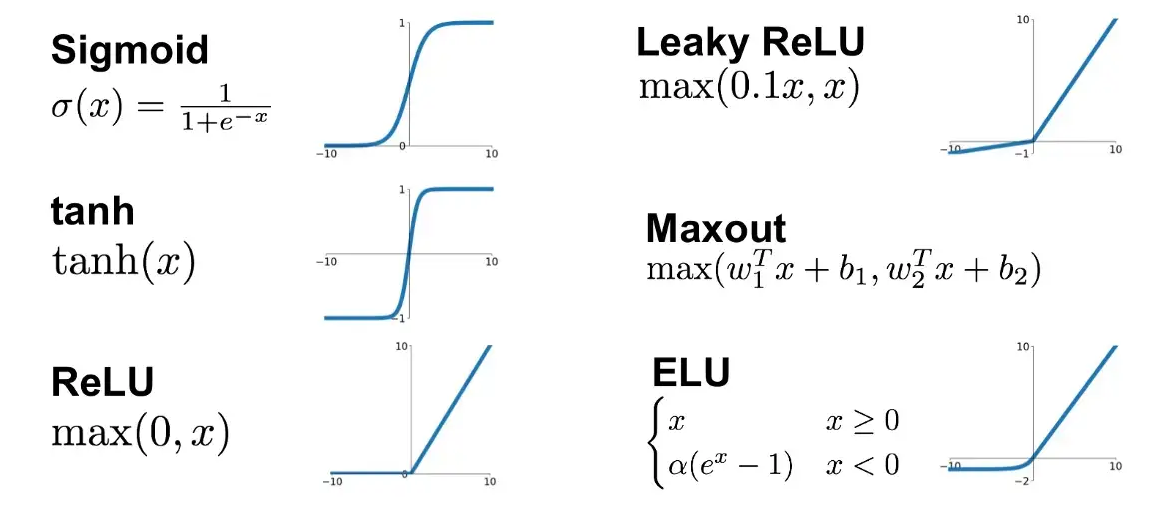
\includegraphics[scale=0.4]{Images/activation-functions.png}
    \caption{Activation functions examples~\cite{ActivationFunctionsImage}.}
    \label{fig:activFun}
\end{figure}

%---------------------------------------------------------------------------

\subsection{Limitations of the MLP Model in Image Processing}
\label{ssec:MLPLimitations}

Traditional multilayer neural networks face challenges when processing images, as highlighted in~\cite{TDS-NNCons}. One major issue is that Multilayer Perceptron (MLP) networks require \textbf{one input perceptron per image pixel} for grayscale images, and for RGB images,  each pixel needs three input perceptrons, leading to three weights per pixel that need to be calculated and stored. This means that for a $224$x$224$ RGB image, over $150,000$ weights need updating, which can significantly increase training time and the risk of overfitting. Overfitting occurs when the network performs well on training data but poorly on new, unseen data.

Additionally, MLP networks struggle when dealing with input images that are \textbf{shifted} or \textbf{rotated}, or when the object of interest appears in \textbf{different locations} across images. For instance, if an object is mostly located in the top left corner in the training data, the network may learn to only recognize objects in that specific part of an image, leading to misclassification when the object appears elsewhere. This problem arises because the network emphasizes connections corresponding to the pixels where the object is most frequently observed.

Another drawback of MLP networks is the loss of \textbf{spatial information} when an image is flattened for MLP model input. Neurons close to each other capture certain image features, making it crucial to preserve spatial information to teach the model to recognize objects regardless of their position in the image. Traditional multilayer neural networks lack this capability, failing to utilize pixel adjacency to identify features that could later be used for object recognition.

%---------------------------------------------------------------------------

\section{Convolutional Neural Networks}
\label{sec:CNNs}

Given that the data used in this research consists of images, this subsection will introduce \textit{Convolutional Neural Networks} (\textit{CNNs}) - a popular type of neural network utilized in image data analysis. CNN's name comes from convolution, which is the main operation used for image feature extraction.

\begin{figure}[!htb]
    \centering
    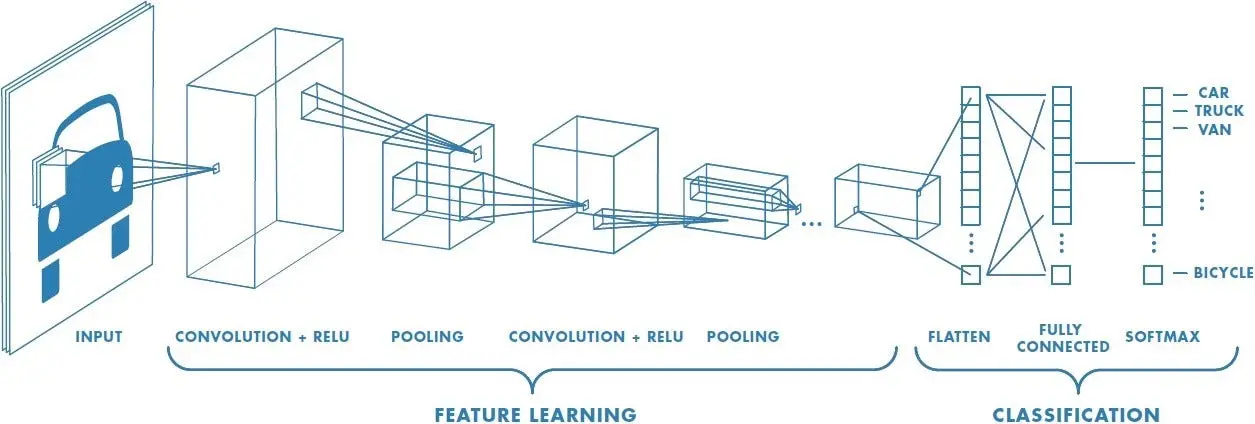
\includegraphics[scale=0.3]{Images/CNN-model.jpg}
    \caption{Convolutional Neural Network~\cite{CNNBlogGuide}.}
    \label{fig:CNNModel}
\end{figure}

Convolutional neural networks allow you to analyze images using \textbf{feature extraction} and \textbf{pattern recognition}. The operation of CNNs can be broken down into the following steps:

\begin{enumerate}
    \item   Initially, \textit{\textbf{image padding}} adds a frame of pixels around the input image, ensuring the dimensions remain the same after convolution.
    \item   A \textit{\textbf{filter}} (usually $3x3$ or $5x5$) detects specific shapes in the input image through \textit{\textbf{convolution}}. It multiplies each pixel in a region by corresponding filter values and sums the results, moving across the image to create \textit{feature maps}. The filter parameters determine the number of feature maps, highlighting areas where the feature is present.
    
    The weight values in filters are calculated automatically, meaning the distinctive features of the objects under analysis are determined during the learning process of the convolutional network.
    \item   Next, \textit{\textbf{activation functions}} are used to remove insignificant information from the feature maps, which speeds up network training by setting negative values (indicating the absence of sought-after features in a given area) to zero or another small value.
    \item   The following step involves \textit{\textbf{pooling}}, with \textit{\textbf{max pooling}} being the most common variant. This involves traversing the feature map with a window and selecting the pixel with the highest value from each neighborhood. For \textit{\textbf{average pooling}}, the average value is used. This value is then used to replace the entire area. This reduces the feature map size while retaining important information.
    \item   The processes of \textit{\textbf{convolution}} and \textit{\textbf{pooling}} are then alternated according to the network's architecture. Each subsequent layer identifies more abstract features. For example, in a plant species recognition network, early layers detect basic elements like edges and textures, while later layers identify detailed attributes such as leaf shape, vein patterns, and the presence of flowers or fruits. Advanced layers integrate these details to distinguish between species, focusing on specific characteristics like leaf shape, flower color, and growth habits.
    \item Finally, the last layer of the convolutional network is \textbf{\textit{fully connected}} and is responsible for the final classification. The input to this layer is flattened from matrices into a vector.
\end{enumerate}

Considering the limitations outlined in section \ref{ssec:MLPLimitations}, it is clear that traditional multilayer neural networks face notable challenges, especially in the context of image processing. Convolutional Neural Networks (CNNs) effectively address these limitations. To illustrate this advancement, each stage of a CNN is analyzed. A detailed analysis showing how each stage directly addresses these limitations is presented in Table \ref{tab:CNNStages}.

It is essential to keep in mind that Convolutional Neural Networks (CNNs), despite their advanced capabilities, \textbf{demand a wide spectrum of training examples} to achieve optimal performance. In cases where the variability among examples is limited, employing \textbf{data augmentation becomes crucial}. This technique is the core of the analysis in this master's thesis. It enables the generation of a diverse set of samples, ensuring that the CNN is well-equipped to handle various scenarios in image analysis.

\begin{table}[H]
    
    \caption{Applications and Functions of Convolutional Network Stages.}
    \centering
    \begin{tabular}{|>{\centering\arraybackslash}m{4cm}|>{\centering\arraybackslash}m{3.9cm}|>{\centering\arraybackslash}m{6.8cm}|}
     
      \hline
     \textbf{Stage} & \textbf{Function} & \textbf{Application}  \\ 
      \hline
      Convolution & Using a filter extracts the features of the object visible in the image. & Enables sparser connections.
      
      Reduces the number of parameters.
      
      Prevents overfitting.
      
      Combined with pooling, it ensures the target object's position in the image does not affect classification.\\ 
      \hline
      Activation Function & Introduces non-linearity. & Improves training and prediction speed. \\

      \hline
      Pooling & Replaces a neighborhood of pixels with a singular value. & Reduces dimensionality. 
      
      Increases robustness to distortions and variability in images as the arrangement of values within the neighborhood becomes irrelevant.\\
      \hline
      Classification & Utilizes a fully connected layer of neurons to predict the final outcome. & Facilitates the recognition of objects that are distinct yet represent the same category, enhancing the network's resilience to a wide array of test cases.\\
      \hline
    
    \end{tabular}
    \label{tab:CNNStages}
\end{table}

%---------------------------------------------------------------------------

\section{Generative Adversarial Networks (GANs)}
\label{sec:GANs}

Generative Adversarial Networks (GANs) are one of the most significant advancements in artificial intelligence and machine learning in the last decade. This chapter explores the foundational concepts, mechanisms, and applications of GANs, which have revolutionized generative modeling and opened new possibilities in areas such as image generation, video synthesis, and more.
%---------------------------------------------------------------------------

\subsection{Introduction to GANs}

Generative Adversarial Networks (GANs) were introduced by Ian Goodfellow et al in 2014~\cite{GANsOriginalPaper}. GAN consists of two distinct models: a \textbf{generator} and a \textbf{discriminator}. These models are trained simultaneously in a zero-sum game framework, where the generator aims to produce realistic data instances, and the discriminator attempts to distinguish between real and generated data. The adversarial nature of this framework drives both models to improve continuously.

In most GAN architectures, both the generator and discriminator consist mainly of convolutional and fully connected layers. The generator is a mapping between a vector of random values (called the latent space) to the space of data (images in our case): $\mathcal{G}: \mathcal{G}(z) \rightarrow \mathcal{R}^{|x|}$ where $z \in \mathbb{R}^{|z|}$ is a sample from the latent space, $x \in \mathbb{R}^{|x|}$ is an image and $| \cdot |$ denotes the number of dimensions. On the other hand, the discriminator may be characterized as a function that maps from image data to a probability that the image comes from the real data distribution. It can be represented as follows: $\mathcal{D}: \mathcal{D}(x) \rightarrow (0, 1)$.

\begin{figure}[!htb]
    \centering
    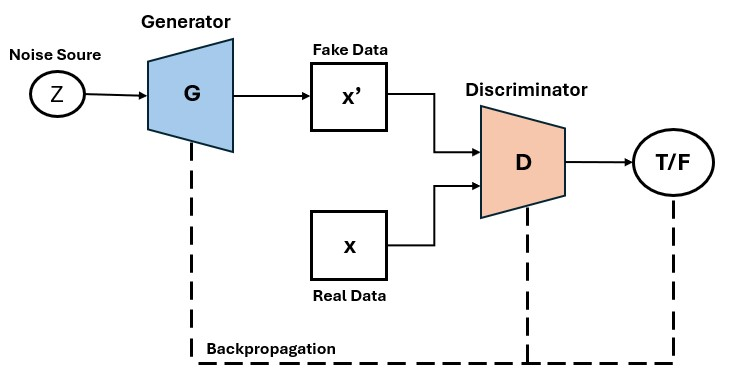
\includegraphics[scale=0.5]{Images/gan_framework.jpg}
    \caption{GAN framework. Inspired by~\cite{GANFramework}.}
    \label{fig:GANFramework}
\end{figure}

As shown in Figure \ref{fig:GANFramework}, the generator does not have direct access to real images. The only way it can learn the high-dimensional distribution behind the data is through interaction with the discriminator which can access both synthetic and real samples. The error signal, derived from a straightforward comparison with the ground truth, can be used to train both the generator and discriminator. By backpropagating this error, the discriminator's ability to classify images improves, and at the same time, the generator's capability to produce higher-quality images is enhanced. Once we are satisfied with the effectiveness of the discriminator, we can stop training it and continue to train only the generator. 
If the distribution created by the generator perfectly aligns with the actual data distribution, then the discriminator should reach its highest level of uncertainty and assign a probability of 0.5 to every input.\cite{GANOverview} The training of GANs is discussed in detail in section \ref{ssec:GANsTraining}.

To address specific challenges and improve generative performance, a variety of architectures have been developed. In the domain of data augmentation, Generative Adversarial Networks (GANs) have emerged as powerful tools for generating synthetic data, enhancing the diversity and volume of datasets. Types of GAN models particularly effective in this domain are presented in section \ref{ssec:typesOfGANs}.

% Particularly effective in this domain are Conditional GANs (cGANs), which can produce images conditioned on specific attributes or classes, thereby enriching category-specific data. CycleGANs also play a crucial role by facilitating image-to-image translation tasks without the need for paired examples, allowing for the augmentation of datasets across different styles or domains. Another significant contribution comes from DCGANs (Deep Convolutional GANs), which leverage convolutional neural networks to generate high-quality images that can mimic various real-world variations.

%---------------------------------------------------------------------------
\subsection{GANs Training}
\label{ssec:GANsTraining}

Training of Generative Adversarial Networks is described in detail in~\cite{GANOverview}. The GAN training is a complex and iterative process that involves optimizing two neural networks — the generator and the discriminator — against each other. This process can be described as a game where the generator's goal is to produce data indistinguishable from source data, while the discriminator's goal is to correctly classify data as real or fake.

To achieve this, a value function $V(G,D)$ is used to update the discriminator and generator in a synchronized fashion. This value function depends on the current state of both networks. Training involves solving a min-max optimization problem where the discriminator tries to maximize its ability to distinguish real data from fake, and the generator tries to minimize the discriminator's accuracy. The standard GAN loss function is described by equations \ref{eq:GANOptimization} and \ref{eq:GANLoss}.
    
\begin{equation}
    \max_{D} \min_{G} V(G, D),
    \label{eq:GANOptimization}
\end{equation}

where

\begin{equation}
    V(G, D) = \mathbb{E}_{x}[\log D(x)] + \mathbb{E}_{z}[\log (1 - D(G(z)))]
    \label{eq:GANLoss}
\end{equation}

This loss function of a Generative Adversarial Network (GAN) guides the training of both components of GANs. It consists of two expressions: the first expression (\(\mathbb{E}_{x}[\log D(x)]\)) measures how well the discriminator recognizes actual data, and the second expression (\(\mathbb{E}_{z}[\log (1 - D(G(z)))])\)) measures the discriminator's ability to detect fake data produced by the generator. Together, they form a tug-of-war where the discriminator improves its detection skills while the generator tries to create increasingly convincing fakes. 

Although this function seems to be useful, in practice, it saturates quickly for the generator, which means that it frequently stops training if it does not keep pace with the discriminator. To address this issue, a refined version of the standard GAN loss employs a strategy where the generator aims to maximize $- log(D(G(z))$. This adaptation focuses on increasing the likelihood of generated images being classified as real rather than decreasing their likelihood of being found fake~\cite{GANEquations}.


The standard GAN loss function can be divided into two parts: \textbf{generator loss} and \textbf{discriminator loss}. During training, the discriminator is typically trained first in each cycle. It is updated to maximize its accuracy on identifying real versus generated data. This is done by feeding it real data and training it to predict ‘real’, and then feeding it fake data from the generator and training it to predict ‘fake’. This step is crucial because a well-trained discriminator guides the generator toward producing more realistic data. The discriminator punishes itself for wrongly identifying a real instance as false, or a false instance (made by the generator) as true, through the maximization of the following function \ref{eq:discrimnator}.

\begin{equation}
    \nabla_{\theta_d} \frac{1}{m} \sum_{i=1}^{m} \left[ \log D \left( x^{(i)} \right) + \log \left(1 - D \left( G \left( z^{(i)} \right)\right)\right) \right]
    \label{eq:discrimnator}
\end{equation}

Subsequently, the generator is updated. It aims to produce data that the current discriminator will classify as real. This is achieved by modifying the generator's parameters in a way that minimizes the output of the discriminator. Ideally, the discriminator should reach a point where it predicts 0.5 for all inputs, indicating it is unable to distinguish between real and fake data. This state indicates that the generator produces highly realistic data. To train the generator, the function in equation \ref{eq:generator} must be minimized. The generator gets rewarded for successfully fooling the discriminator and gets penalized otherwise. 

\begin{equation}
    \nabla_{\theta_g} \frac{1}{m} \sum_{i=1}^{m} \log \left(1 - D \left( G \left( z^{(i)} \right)\right)\right)
    \label{eq:generator}
\end{equation}

However, training GANs can be unstable, and convergence is not always guaranteed. The networks may end up in a situation where the generator produces a limited range of outputs, or the discriminator may become too effective too quickly, leaving the generator with no meaningful gradient to learn from. To address these issues, techniques such as \textbf{feature matching} and \textbf{minibatch discrimination} have been proposed. These methods stabilize the training process by ensuring that the generator produces diverse outputs, and the discriminator evaluates batches of data instead of individual samples~\cite{GANOverview}.


\begin{figure}[!htb]
    \centering
    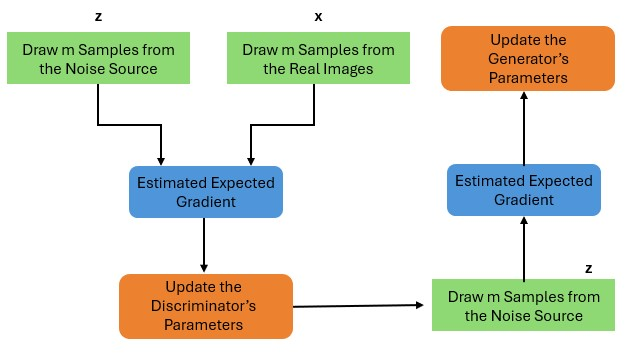
\includegraphics[scale=0.65]{Images/gan-training.jpg}
    \caption{GANs training. Inspired by~\cite{GANOverview}.}
    \label{fig:GANTraining}
\end{figure}

\subsection{Types of GANs}
\label{ssec:typesOfGANs}

This section explores several main types of Generative Adversarial Networks (GANs), each serving distinct purposes and exhibiting unique characteristics. The information presented here is based on an article that provides an overview of GANs~\cite{GANOverview}.

\textbf{Standard GANs}: First, we have Standard GANs. These initial GAN architectures used fully connected neural networks for both the generator and discriminator. Standard GANs were applied to simpler datasets like MNIST, CIFAR-10, and the Toronto Face Dataset, and they set the foundation for more complex models.

\textbf{Deep Convolutional Generative Adversarial Networks (DCGANs)}: DCGANs were introduced to bridge the gap between the success of Convolutional Neural Networks (CNNs) in supervised learning (mentioned in Section \ref{sec:CNNs}) and their potential in unsupervised learning. The original DCGAN paper~\cite{OriginalDCGAN} detailed how DCGANs apply CNN architectures shown in Figure \ref{fig:DCGANsFlow}, which are successful in tasks like image classification, to the generative model of GANs. This allows for robust learning of \textbf{feature hierarchies} and more detailed and nuanced image generation.


\begin{figure}[!htb]
    \centering
    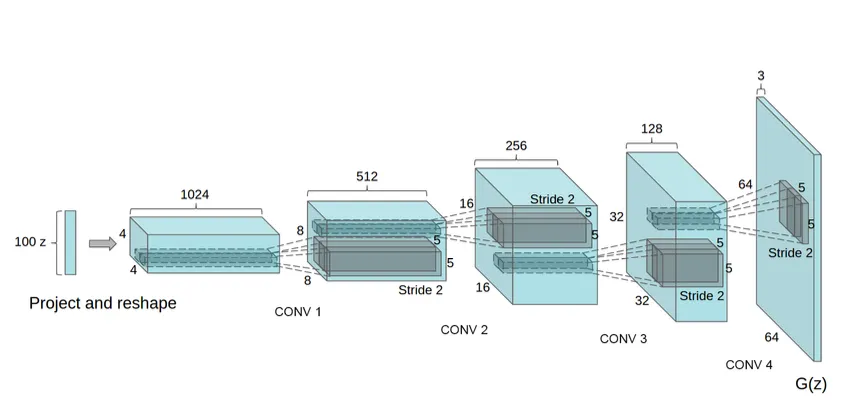
\includegraphics[scale=0.4]{Images/DCGAN-example.jpg}
    \caption{DCGANs flow~\cite{DCGANsFlow}.}
    \label{fig:DCGANsFlow}
\end{figure}

Additionally, DCGANs propose several key architectural innovations to promote stable training of GANs, particularly for generating high-resolution images. These innovations include:
\begin{enumerate}
    \item \textbf{Replacing Pooling Layers}: DCGANs replace pooling layers with strided convolutions in the discriminator and fractional-strided convolutions in the generator. This helps the networks learn their own spatial hierarchies.
    \item \textbf{Using Batch Normalization}: This technique is applied across the entire network, with the exception of the generator's output layer and the discriminator's input layer. It standardizes the inputs to each unit, mitigating the internal covariate shift problem and stabilizing training dynamics.
    \item \textbf{Eliminating Fully Connected Layers}: DCGANs suggest removing fully connected hidden layers to rely entirely on convolutional layers to improve training and reduce the risk of overfitting.
    \item \textbf{Activation Functions}: The generator uses the ReLU activation function in all layers except for the output, which uses the Tanh function. This encourages the model to learn faster and cover the color space more effectively. The discriminator employs the LeakyReLU activation for better gradient flow, especially beneficial when dealing with higher-resolution images.
\end{enumerate}

\textbf{Conditional Generative Adversarial Networks (cGANs)}: cGANs are a type of GANs that are specifically designed to generate output data in a \textbf{controlled manner}. Unlike standard GANs that generate data without a specific direction, cGANs utilize additional label information to guide the generation process. This involves modifying both the generator and discriminator to accept label data (y), allowing the network to condition its outputs on these labels. The mathematical framework of cGANs extends the standard GAN formula by incorporating conditional probabilities, which align the generated outputs with predefined labels. This mechanism not only accelerates the convergence of the network but also allows for control over the characteristics of the generated images at testing time, making cGANs highly effective for tasks requiring specified outputs, such as data augmentation~\cite{cGANs}. You can refer to Figure \ref{fig:cGANsFramework} for a better understanding of the cGANs framework. The cGANs framework is useful for tasks that require generating targeted data outputs.

\begin{figure}[!htb]
    \centering
    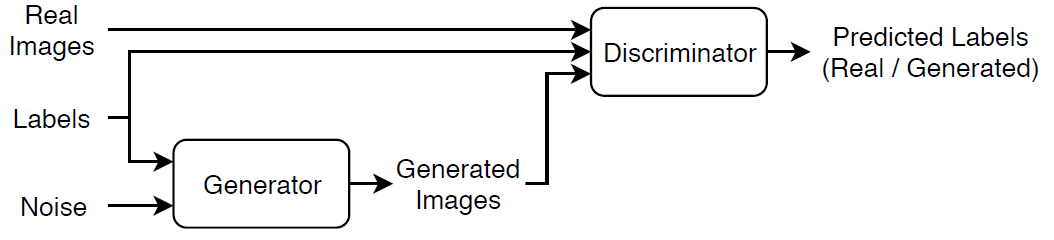
\includegraphics[scale=0.35]{Images/cgan-diagram.png}
    \caption{Conditional GANs framework~\cite{cGANs}.}
    \label{fig:cGANsFramework}
\end{figure}

\textbf{CycleGAN}: CycleGANs are a type of neural network that can perform image-to-image translation without the need for paired examples. This is achieved through the use of two generators and two discriminators that work together to map images from one domain to another. What makes CycleGANs stand out is the incorporation of Cycle Consistency Loss, which ensures that an image converted from one domain back to its original domain retains its original features. This means that transformations, such as turning a horse into a zebra (Figure \ref{fig:cycleGANsExample}), can be reversed. CycleGANs are ideal for tasks without paired training data, marking a significant advance in unsupervised learning~\cite{cycleGANs}.

\begin{figure}[!htb]
    \centering
    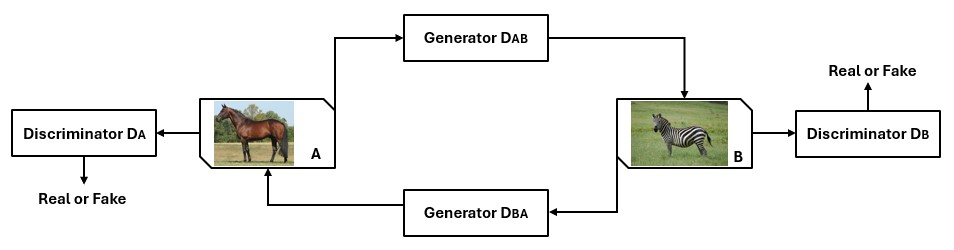
\includegraphics[scale=0.62]{Images/cycleGANexample.jpg}
    \caption{CycleGANs example described in this section. Based on~\cite{cycleGANs}.}
    \label{fig:cycleGANsExample}
\end{figure}

\textbf{StyleGANs}: StyleGANs, developed by NVIDIA, are explained in detail in this article~\cite{StyleGAN}. They integrate and extend the progressive training methodology of ProGAN~\cite{ProGAN}. This methodology scales up image resolution from lower to higher during the training process, which enhances stability and image quality throughout the training phase. 

StyleGANs have a style-based generator that separates high-level attributes (like pose and identity) from stochastic variations (like skin texture or hair details) within images. This separation is achieved through an intermediate latent space that allows the manipulation of styles at different levels of the synthesis network, using a technique called Adaptive Instance Normalization (AdaIN). Each level of detail, from coarse to fine, can be adjusted independently without affecting other levels. This provides unprecedented control over the synthesis process.

\begin{figure}[!htb]
    \centering
    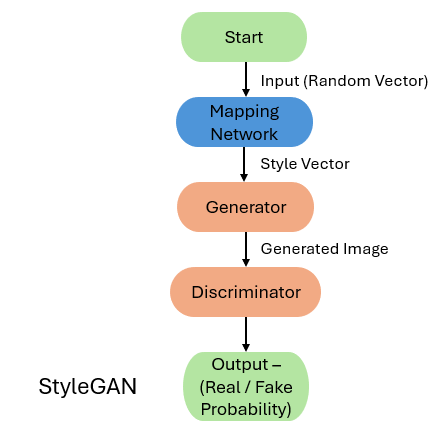
\includegraphics[scale=0.63]{Images/style-gan-high-level.png}
    \caption{StyleGAN - High-Level overview. Inspired by~\cite{StyleGANHighLevel}.}
    \label{fig:styleGANHighLevel}
\end{figure}

Moreover, StyleGAN enhances feature control through a mapping network that converts input vectors into an intermediate latent space. This space more effectively disentangles factors of variation, allowing for easier manipulation of individual features without affecting others. This capability makes StyleGAN not only a powerful tool for generating highly realistic images but also improves its ability to perform targeted modifications and explorations of the generative space. A high-level overview of StyleGAN's functionality is visualized in Figure \ref{fig:styleGANHighLevel}.

The features of StyleGAN technology have placed it at the forefront of GAN technology. It has pushed the limits of how artificial images can be refined and controlled for tasks that require high levels of detail and realism. The model's ability to generate nuanced, customizable images has broad implications for fields ranging from digital content creation to training data enhancement for machine learning algorithms. Examples of images generated by StyleGAN are shown in Figure \ref{fig:styleGANExample}.

\begin{figure}[!htb]
    \centering
    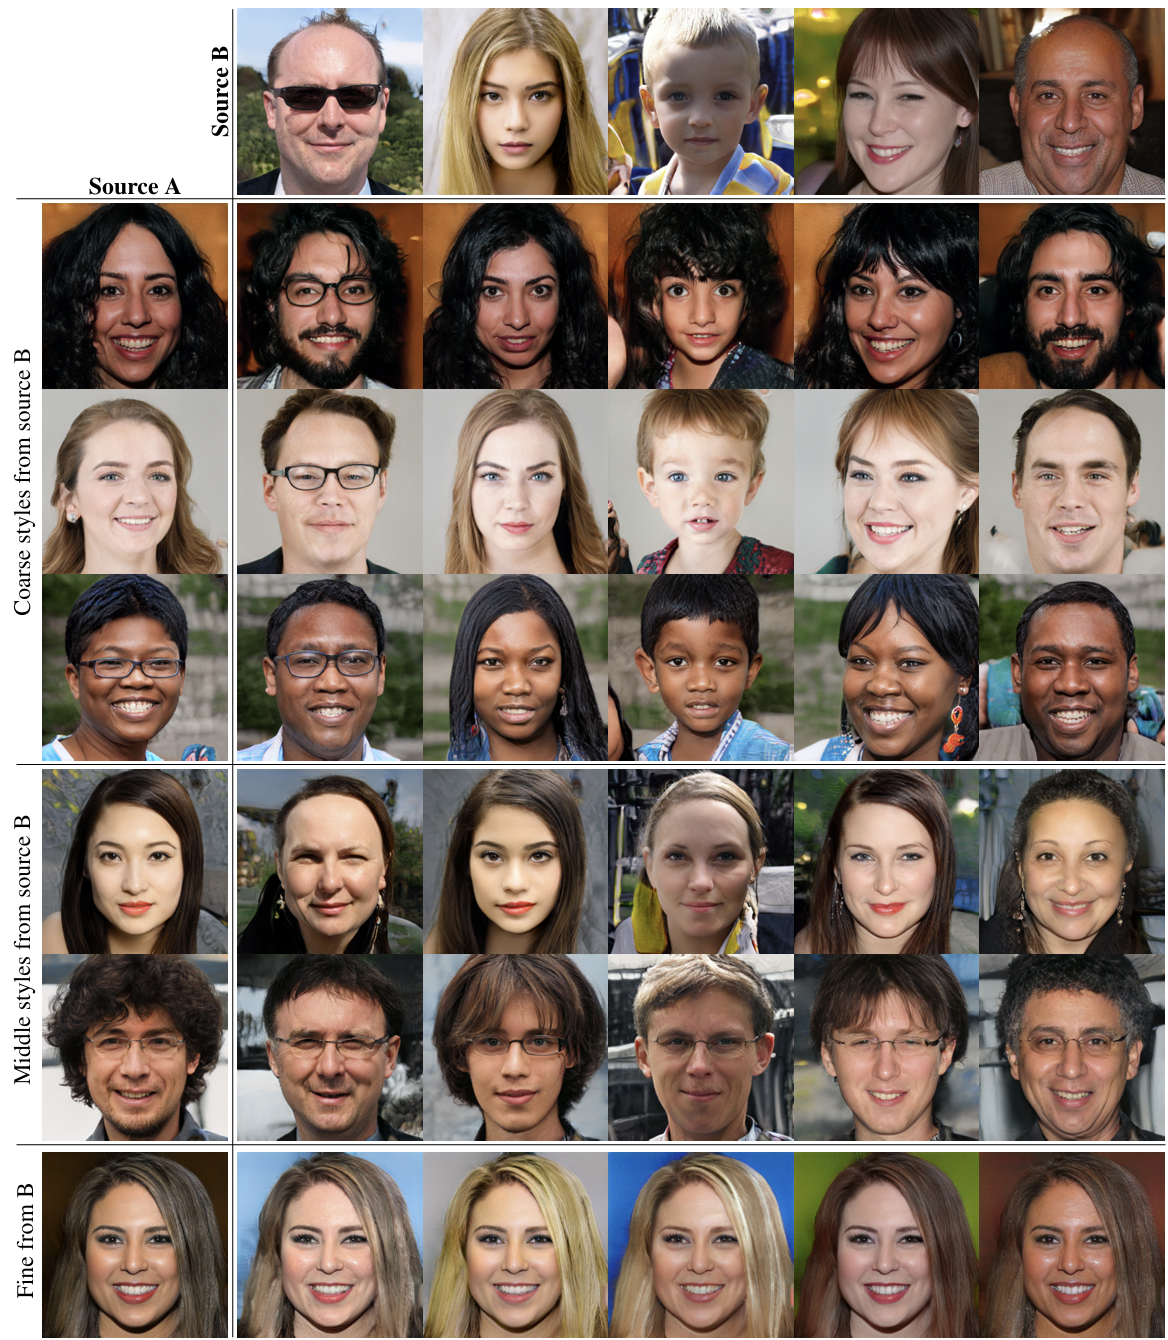
\includegraphics[scale=0.6]{Images/style-gan-example.png}
    \caption{Examples of images created by StyleGAN. Images were generated from two latent spaces: Source A and B. A particular subset of styles was then transferred from Source B to Source A. Depending on the resolution of the styles transferred, different degrees of change were achieved in the images. When coarse styles were copied from Source B to A, the gender and age of the images were preserved. If middle-resolution styles were transferred, smaller facial features, hairstyles, and eye openness from Source B were inherited by the images from Source A. However, the general face shape, pose, and eyeglasses from Source A were still preserved. For fine-grained styles, only minor changes such as hair color were applied~\cite{cycleGANs}.}
    \label{fig:styleGANExample}
\end{figure}

%---------------------------------------------------------------------------

\section{Transfer Learning}
\label{sec:transferLearning}
Transfer learning was first introduced by Stevo Bozinovski in 1976, with the original article written in Croatian. In 2020, a follow-up article was published, providing a detailed mathematical and geometric theory related to transfer learning~\cite{TransferLearningFirst}.

This subsection draws insights from the book~\cite{TransferLearning}, which extensively explores both the theoretical aspects and practical implementations of transfer learning, particularly using the Python programming language. The aim is to provide a comprehensive discussion on the topic.

The core concept of transfer learning, illustrated in Figure \ref{fig:transferLearning}, is based on the principle of leveraging existing knowledge to master new tasks. It is similar to learning a new language - if you are proficient in Spanish, you will find it easier to learn Portuguese due to the similarities between the two languages. Similarly, we can take advantage of established network architectures (like \textit{EfficientNet}), which have been previously trained on vast datasets. This approach is beneficial because the initial layers of convolutional networks are trained to identify simple visual features. By modifying the architecture's last few layers with new, adjustable parameters aimed at recognizing more complex features specific to a new task, we can rapidly create an effective neural network.

\begin{figure}[!htb]
    \centering
    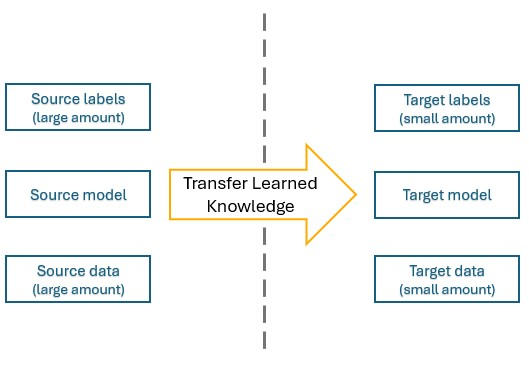
\includegraphics[scale=0.8]{Images/transfer-learning.jpeg}
    \caption{Idea behind transfer learning~\cite{TransferLearningExample}.}
    \label{fig:transferLearning}
\end{figure}

Initially, a well-known model trained on a comprehensive dataset is selected. In the case of images, the ImageNet dataset is often used. It includes around 14 million images, categorized into more than 20,000 categories. The next step is to decide which of the trained weights to freeze, preventing their values from changing. Typically, initial layers weights from the base model are frozen to accelerate the learning process. The next phase involves appending a new model on top of the pre-trained network. The weights of this new model are not fixed but are instead fine-tuned to address the specific characteristics of our dataset. This results in a strong multi-layered model with minimal time investment.

%---------------------------------------------------------------------------

\section{Pre-trained Models}
\label{sec:pretrainedModels}

%---------------------------------------------------------------------------

\subsection{ResNet}

Introduced in 2015, the \textit{ResNet} architecture (short for \textit{Residual Networks}) is detailed in the study~\cite{DeepResidualLearning} by \textit{Kaiming He et al.}, which serves as a key reference throughout this subsection. The developers of this technique identified that a more efficient strategy than extending successive identity connections is to skip over a few connections while assigning near-zero values to filters and then aggregating the results of these processes, as illustrated in Figure \ref{fig:resNetSkipConnections}. This technique enables the emulation of the identity function, which helps to avoid the vanishing gradient problem when necessary.

\begin{figure}[!htb]
    \centering
    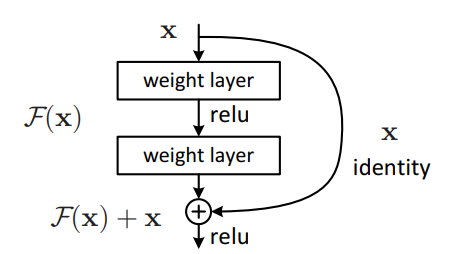
\includegraphics[scale=0.5]{Images/skip-connection.png}
    \caption{Skip-connections~\cite{DeepResidualLearning}.}
    \label{fig:resNetSkipConnections}
\end{figure}

The \textit{ResNet} network is designed with residual connections every few layers. Figure \ref{fig:CNNcomparision} compares the architecture of the \textit{VGG-19} network, a standard 34-layer convolutional network, and a 34-layer residual network.

\begin{figure}[!htb]
    \centering
    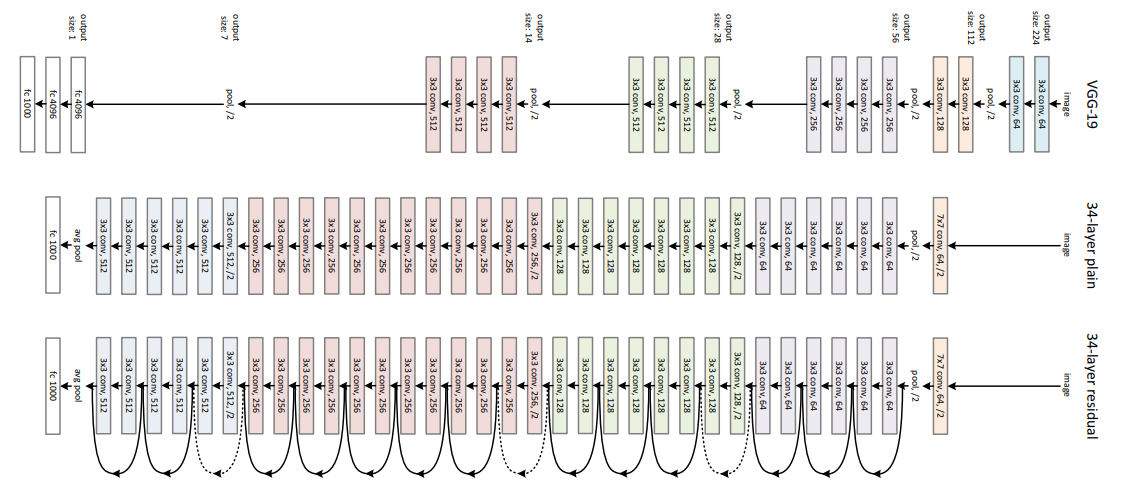
\includegraphics[scale=0.4]{Images/34-layers-nets-comparision.png}
    \caption{CNN architectures comprasion~\cite{DeepResidualLearning}.}
    \label{fig:CNNcomparision}
\end{figure}

The use of residual connections allows for building deeper architectures without vanishing gradient problems (Figure \ref{fig:ResNetLearningCurves}). Notably, even though \textit{ResNet} networks can have up to 152 layers, they are less complex than \textit{VGG} networks with 19 layers due to the implementation of residual connections. Specifically, \textit{ResNet-152} performs approximately $11.3$ billion addition/multiplication operations, whereas \textit{VGG-19} requires about $19.6$ billion operations.

\begin{figure}[!htb]
    \centering
    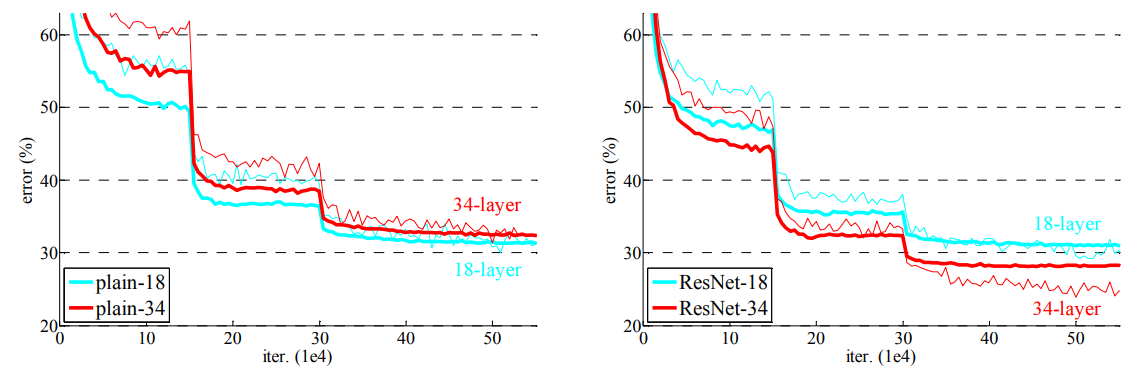
\includegraphics[scale=0.5]{Images/res-net-learning-curves.png}
    \caption{Comparison of learning curves of simple and residual networks~\cite{DeepResidualLearning}.}
    \label{fig:ResNetLearningCurves}
\end{figure}


In conclusion, as more layers are added, \textit{ResNet} networks demonstrate improved performance until overfitting occurs. The effectiveness of residual connections increases with the network's depth. For \textit{ResNet} architectures with more than 34 layers, special structures known as \textit{bottleneck} designs are commonly employed to enhance computational efficiency, as illustrated in Figure \ref{fig:bottleNeck}. These designs consist of three layers: a dimension-reducing layer (1x1 filter), a feature-detecting layer (3x3 filter), and a dimension-restoring layer (1x1 filter). This arrangement allows the feature-detecting layer to operate on a reduced dimensionality, thereby speeding up the computational process.

\begin{figure}[!htb]
    \centering
    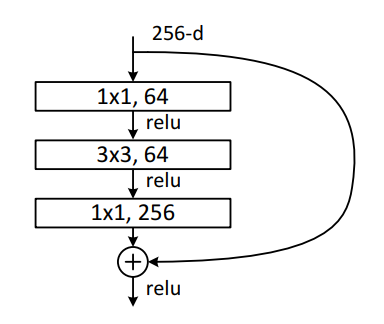
\includegraphics[scale=0.5]{Images/bottle-neck.png}
    \caption{Bottle-neck structure used in \textit{ResNet} networks~\cite{DeepResidualLearning}.}
    \label{fig:bottleNeck}
\end{figure}

%---------------------------------------------------------------------------

\subsection{EfficientNet}

The paper "EfficientNet: Rethinking Model Scaling for Convolutional Neural Networks"~\cite{EfficientNet} was published in 2019 and introduced the convolutional network called \textit{EfficientNet}. The authors focused on analyzing the efficiency of scaling various dimensions of convolutional networks and its impact on performance. The information from this paper has been utilized in writing this chapter.

\begin{figure}[!htb]
    \centering
    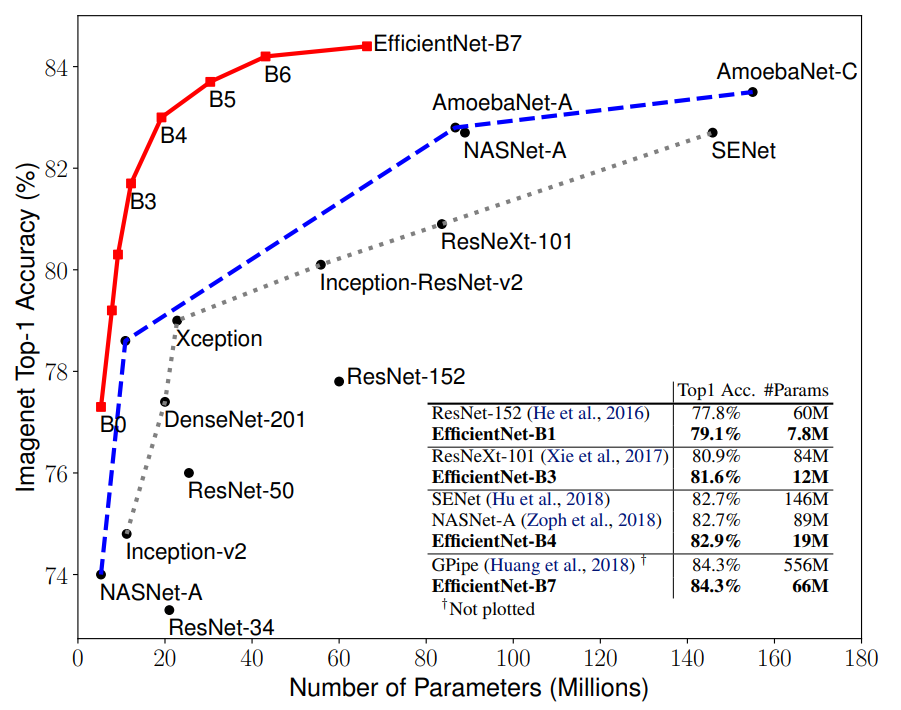
\includegraphics[scale=0.45]{Images/efficient-net-accuracy.png}
    \caption{Precision of EfficientNet compared to other known architectures~\cite{EfficientNet}.}
    \label{fig:efficientNet}
\end{figure}

As observed in Figure \ref{fig:efficientNet}, the \textit{EfficientNet} architecture outperforms other well-known network architectures in terms of accuracy on the \textit{ImageNet} dataset while maintaining a relatively low parameter count. The graph compares successive versions of the \textit{EfficientNet} network with other architectures that offer similar accuracy levels. It turns out that in every comparison, \textit{EfficientNet} operates with significantly fewer parameters. For instance, \textit{EfficientNet-B7} achieves the same accuracy as the \textit{GPipe} network but is described by more than 8 times fewer parameters, making it over 6 times faster.

\textit{EfficientNet} is built around the idea of strategic model scalability, which is achieved through adjustments in three key dimensions:
\begin{enumerate}
    \item Network \textbf{width} (the number of convolutional network filters)
    \item Network \textbf{depth} (the number of hidden layers)
    \item Input image \textbf{resolution}
\end{enumerate}

\begin{figure}[!htb]
    \centering
    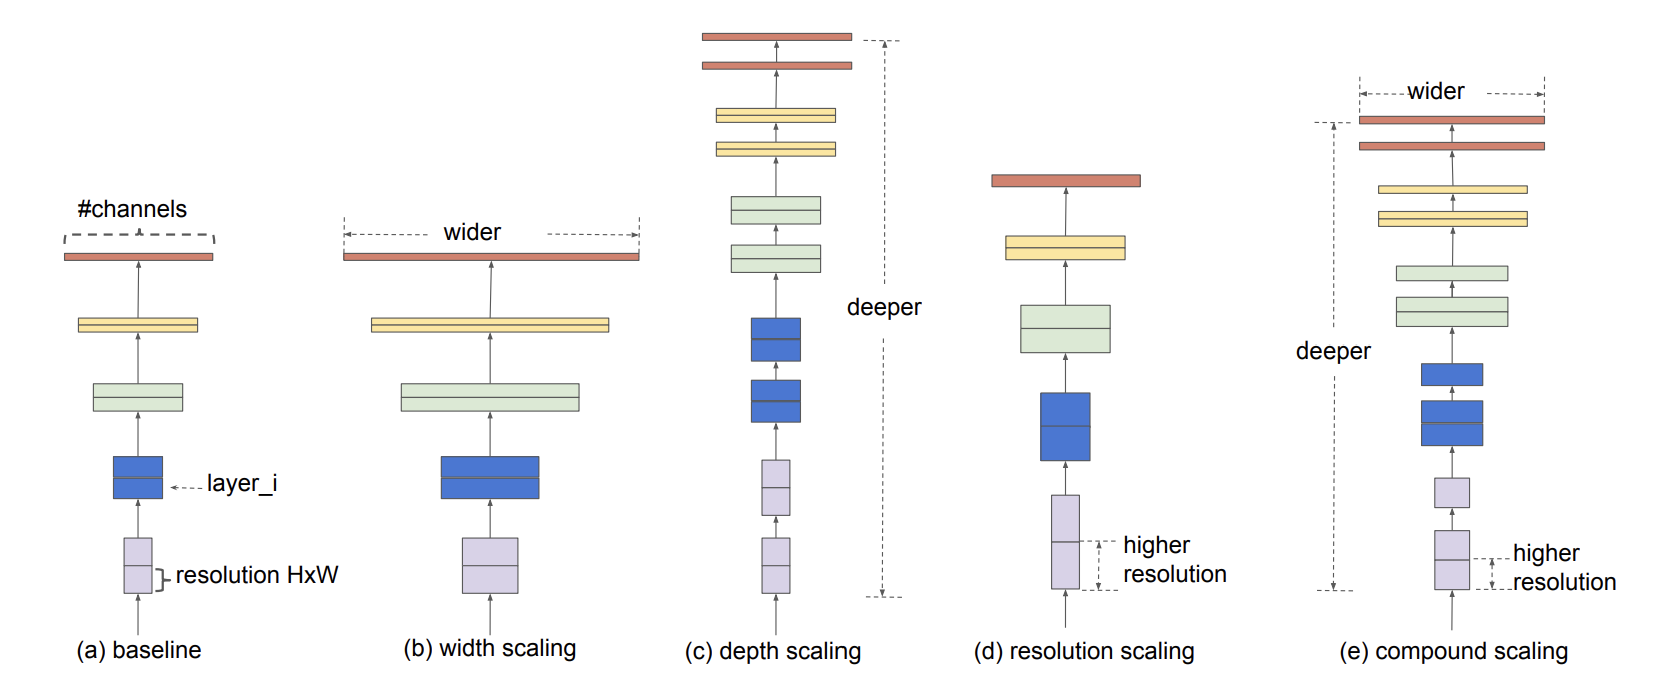
\includegraphics[scale=0.7]{Images/efficient-net-model-scaling.png}
    \caption{Model Scaling. (a) a baseline network example; (b)-(d) are conventional scaling - one dimension of a network at a time: width, depth, or resolution. (e) compound scaling method that scales all three dimensions with some fixed ratio~\cite{EfficientNet}.}
    \label{fig:modelScaling}
\end{figure}

This concept is illustrated in Figure \ref{fig:modelScaling}. The authors observed that scaling the network in \textbf{all dimensions simultaneously} yields the best results and proposed a novel approach known as the \textbf{compound scaling} method, which utilizes a parameter denoted by $\phi$, as follows:

\begin{equation}
    \begin{cases}
      depth: d = \alpha^\phi\\
      width: w = \beta^\phi\\
      resolution: r = \gamma^\phi
    \end{cases}\,
    \label{eqs:scaling}
\end{equation}

Under the assumptions that $\alpha \cdot \beta^2 \cdot \gamma^2 \approx 2$ and $\alpha \geq 1$, $\beta \geq 1$, $\gamma \geq 1$, where $\alpha$, $\beta$, and $\gamma$ can be determined through a manual grid search of small value sets. Intuitively, $\phi$ represents a parameter that signifies the amount of computational resources available for allocation, while the parameters $\alpha$, $\beta$, and $\gamma$ dictate how these resources are distributed across each dimension.

To significantly improve network performance using the scaling method described above, it is also essential that the foundational architecture (\ref{fig:modelScaling}) is appropriate. To create the EfficientNet, the authors specified a base architecture primarily composed of \textbf{mobile inverted bottleneck modules} (Figure \ref{fig:efficientNetBasicModel}). Then, they refined its architecture through the following steps:
\begin{enumerate}
    \item \textbf{Step 1}: They set the parameter $\phi = 1$, assuming the availability of double the computational resources, and carried out a grid search for the parameters $\alpha$, $\beta$, and $\gamma$. This process identified the most optimal values for these parameters within the base model as 1.2, 1.1, 1.15, under the constraint $\alpha \cdot \beta^2 \cdot \gamma^2 \approx 2$.
    \item \textbf{Step 2}: The parameters $\alpha$, $\beta$, and $\gamma$ were kept constant, and the base network was scaled using different values of $\phi$, following the scaling equation \ref{eqs:scaling}.
\end{enumerate}

\begin{figure}[!htb]
    \centering
    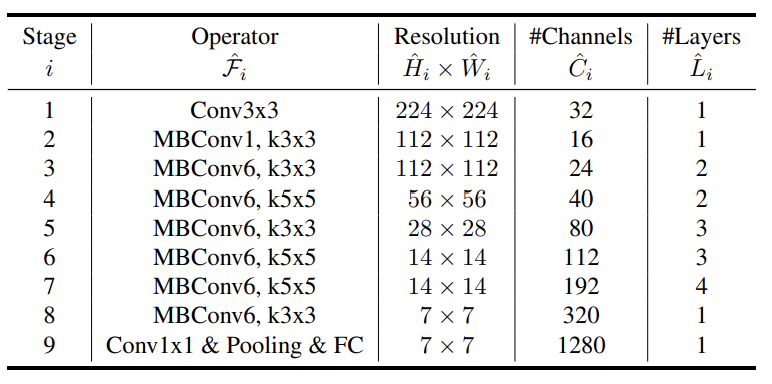
\includegraphics[scale=1]{Images/efficient-net-base-model.png}
    \caption{Baseline models used in \textit{EfficientNet}~\cite{EfficientNet}.}
    \label{fig:efficientNetBasicModel}
\end{figure}

The authors used saliency maps to assess the performance of the trained models. They found that scaling the dimensions of the network in each dimension separately improved the performance of the network, but the scaling method used in EfficientNets resulted in networks focusing on the most important parts of the input image during classification.
	\chapter{Data Augmentation Techniques}
\label{cha:overviewOfDataAugmentation}

%---------------------------------------------------------------------------

Data augmentation is a technique used to increase the diversity of data available for training models without collecting new data. This method involves applying various transformations to existing data samples to create altered versions. This method involves making changes to existing data samples by applying various transformations such as rotations, scaling, cropping, and adjusting lighting conditions. The goal of data augmentation is to make the resulting model more robust, which reduces the likelihood of overfitting and improves its ability to generalize to new, unseen data~\cite{ImageDataAugmentationSurvey}. 

In this chapter, available methods of image augmentation are introduced and the reasons for using data augmentation are explained. The classification of augmentation methods is shown in Figure \ref{fig:augDiagram}.

\begin{figure}[!htb]
    \centering
    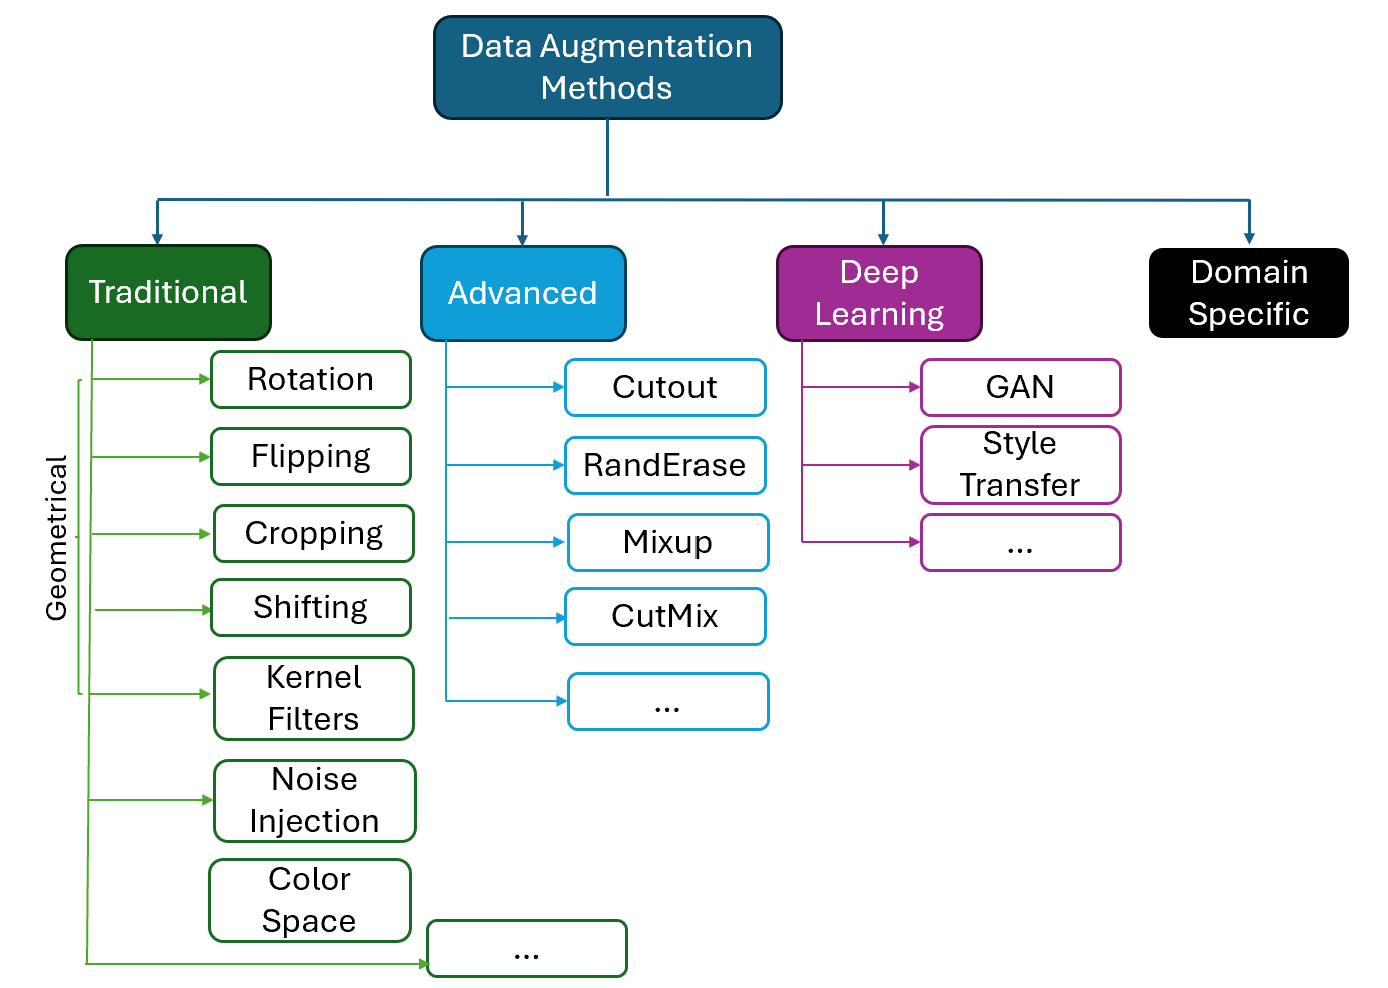
\includegraphics[scale=0.8]{Images/augmentation-diagram.png}
    \caption{Diagram showing the classification of augmentation methods. \\ Inspired by~\cite{AugmentationDiagram}.}
    \label{fig:augDiagram}
\end{figure}

\section{Why Data Augmentation is Essential}

Image data augmentation is an essential technique in the field of deep learning, particularly in tasks involving image recognition and classification. In this section, the reasons and justifications for employing image data augmentation will be explored, deriving insights from Suorong Yang's survey~\cite{DataAugmentationEssential} while integrating additional perspectives from related studies.

\textbf{Handling Overfitting}. One of the primary motivations for using image data augmentation is to reduce overfitting. Overfitting occurs when a model learns the details and noise in the training data to the extent that it negatively impacts the performance of the model on new, test data. By artificially enhancing the dataset through transformations like rotation, scaling, and flipping, the diversity within the training dataset increases. This diversity helps the model generalize better to new, unseen images, therefore improving its predictive performance.

\textbf{Enhancing the Dataset without Additional Data Collection}. Deep neural networks often require large amounts of training data to prevent overfitting. However, obtaining labeled data for real-world applications can be challenging due to its scarcity. Data collection is often a resource-intensive process, requiring significant time, effort, and sometimes financial investment, especially for tasks requiring large annotated datasets. Image data augmentation provides a cost-effective method to expand the dataset without the need for additional data collection.

\textbf{Increasing Model Robustness} Another key aspect of data augmentation is its role in increasing the robustness of models. By exposing the model to a wide range of variations in the data and deformations of objects within the images, the model learns to identify the essential features of the objects regardless of their presentation. This capability is crucial for practical applications where the conditions under which images are captured can vary widely.

The methods described in the subsequent sections are frequently combined by setting a minimal threshold, in the form of a probability, for each method to occur. This approach ensures that each augmentation technique, such as rotations, flips, or color adjustments, is applied selectively rather than uniformly across all images. By doing so, it introduces a stochastic element to the augmentation process, enhancing the diversity of the training data and preventing the model from overfitting to specific attributes of the training set.
%---------------------------------------------------------------------------

\section{Traditional Data Augmentation}
\label{ssec:augmentationTraditional}

The chapter on traditional data augmentation in Conor Shorten's article "A Survey on Image Data Augmentation for Deep Learning"~\cite{ImageDataAugmentationSurvey} provides a comprehensive overview of conventional techniques used in data augmentation to enhance the robustness and generalizability of deep learning models. This article will be used as a reference when writing this subsection of the paper.
%---------------------------------------------------------------------------

\subsection{Basic Transformations}
\label{ssec:basicTransformations}


Traditional basic data augmentation methods are foundational in training deep learning models, particularly in the field of image processing. These techniques involve simple yet effective transformations to existing images in a dataset, aiming to simulate the variability that these models will encounter in real-world scenarios. Key techniques include:


\textbf{Rotation}: involves rotating each image through various angles. This process ensures diverse orientations in the dataset, fostering the model's ability to recognize objects regardless of their rotational position. Maximum rotation degree can be defined.

\textbf{Flipping}: Images are flipped horizontally or vertically. 

\textbf{Random Cropping}: Parts of images are cropped and resized to their original dimensions, teaching the model to focus on different parts of an image. A crop size smaller than the original is defined, and during training, a random starting point is selected to extract a sub-section of the image. This exposes the model to diverse sections of the image, leading to better performance.

\textbf{Shifting}: This technique involves translating the contents of an image in the horizontal or vertical direction to avoid positional bias. This manipulation simulates the effect of objects being located in different parts of the image frame, which can be crucial in tasks where object-varying localization is key.

\textbf{Kernel Filters}: Kernel filters are widely utilized in image processing to sharpen or blur images. These filters apply an n × n matrix over an image using a Gaussian blur filter to create a softer appearance or a vertical or horizontal high-contrast edge filter to enhance sharpness, particularly along edges. Using blurring in data augmentation can increase a model's tolerance to motion blur when deployed. Similarly, sharpening during data augmentation can help highlight finer details in objects.

\textbf{Noise injection}: This technique involves adding random noise (typically Gaussian) to images to mimic real-world imperfections. It helps to build noise-robust models and prevent misclassification of real-world test data, especially if the training dataset consists only of perfect images.

\textbf{Color space}: Changing color helps in training models to be invariant to color changes. Techniques such as adjusting brightness, contrast, saturation, and hue are commonly used. A simple color augmentation technique can rely on isolating one channel R, G, or B and adding two zero matrices

\begin{figure}[!htb]
    \centering
    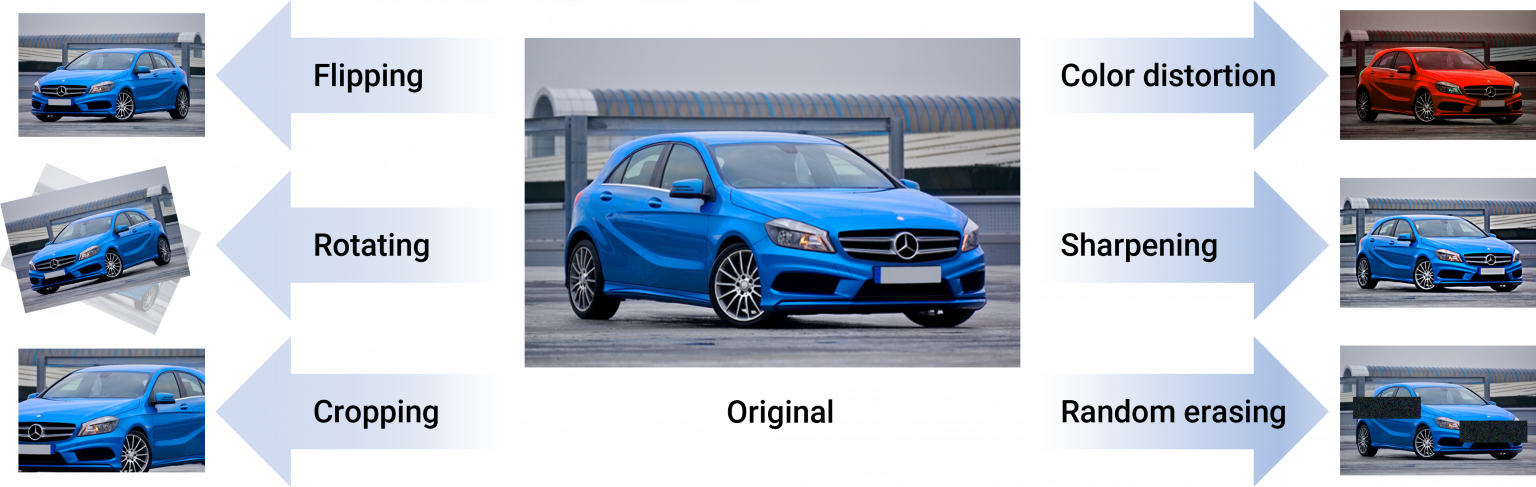
\includegraphics[scale=0.38]{Images/traditional-augmentation-examples.png}
    \caption{Traditional image augmentation examples~\cite{TradAugExamples}.}
    \label{fig:tradAugExamples}
\end{figure}
%---------------------------------------------------------------------------

\subsection{Advanced Transformations}
\label{ssec:advancedTransformations}
%---------------------------------------------------------------------------

\textbf{MixUp}: \textit{MixUp} is a data augmentation technique proposed by Hongyi Zhang et al.~\cite{MixupOriginal} that creates synthetic training examples by linearly combining pairs of images and their labels from the training data. Given two examples \( (x_i, y_i) \) and \( (x_j, y_j) \), the Mixup generated new example \( (\hat{x}, \hat{y}) \) is calculated as follows:
\begin{align*}
    \hat{x} &= \lambda x_i + (1-\lambda) x_j \\
    \hat{y} &= \lambda y_i + (1-\lambda) y_j
\end{align*}
where \( \lambda \) is a mixing coefficient sampled from a Beta distribution, typically \( \text{Beta}(\alpha, \alpha) \) for some \( \alpha > 0 \). By creating virtual examples that blend features and labels of multiple training instances, \textit{MixUp} encourages the model to learn more invariant and robust features which leads to smoother decision boundaries, reducing the likelihood of overfitting.


\textbf{CutMix}: The \textit{CutMix} method, described in~\cite{CutMixOriginal} is a data augmentation technique similar to \textit{MixUp}, but focusing on promoting localization capabilities to improve classification performance. \textit{CutMix} involves cutting parts of images and pasting them onto other images, effectively blending the features of two different classes within a single training example. The corresponding labels are also mixed proportionally to the area of the patches.

\textbf{CutOut}: Also known as \textbf{Random Erasing}, this data augmentation technique involves randomly removing or "cutting out" one or more rectangular regions from an input image during training. This forces the neural network to focus on less dominant features, enhancing its generalization ability. By limiting access to full information, CutOut encourages the model to learn more features of objects, not only the obvious ones. For example, even when only the stem of a flower is visible, the model can still identify the flower, demonstrating its ability to recognize crucial but less prominent features. Seeing the whole flower model would probably focus on the bloom not paying attention to the stem.

\begin{figure}[!htb]
    \centering
    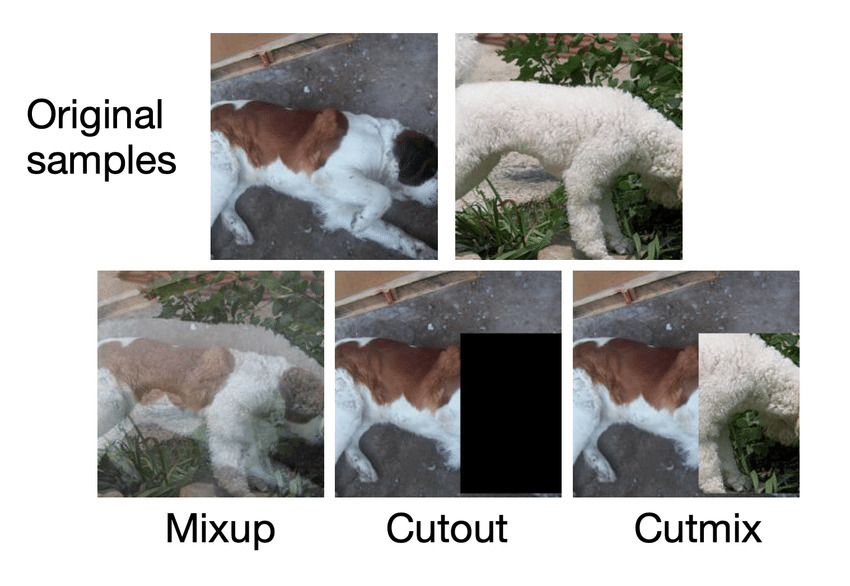
\includegraphics[scale=0.4]{Images/advanced-augmentation-methods.jpg}
    \caption{Advanced image augmentation examples~\cite{AdvAugExamples}.}
    \label{fig:advAugExamples}
\end{figure}

\section{Data Augmentation Using GANs}
\label{ssec:augmentationGANs}

In Section \ref{ssec:typesOfGANs}, the various types of Generative Adversarial Networks (GANs) were described. In this section, the focus will be on how GANs can help synthesize new, realistic data samples to expand existing datasets.

Generative Adversarial Networks (GANs) are leveraged for data augmentation by \textbf{synthesizing new, realistic data samples} that expand existing datasets. This capability is particularly valuable in fields where data collection is challenging or costly. GANs are sometimes described as a way to “unlock” additional information from a dataset. By generating diverse and high-quality artificial samples, GANs improve the robustness of machine learning models, helping them perform better in real-world applications by providing a richer and more varied training environment. Among the variety of GAN models, DCGANs, Conditional GANs, StyleGANs, and CycleGANs are particularly notable for their extensive potential in enhancing data augmentation efforts. 

\textbf{Conditional GANs}: cGANs are particularly useful for data augmentation in classification tasks by generating data samples conditioned on specific labels or attributes. By conditioning the generation process on specific labels, cGANs can produce diverse and representative samples across various classes, addressing \textbf{class imbalance} effectively.  For instance, in a scenario where certain classes are underrepresented, cGANs can generate additional samples for these classes, thereby improving the robustness of classification models. This targeted augmentation helps in achieving more accurate and generalizable classification outcomes in areas such as image recognition and medical diagnostics. For instance, cGANs were successfully used in this paper~\cite{cGANSAugmentation} for improving the Facial Emotion Recognition capabilities of the CNN.

\textbf{StyleGANs}: StyleGANs are particularly effective for data augmentation due to their ability to manipulate and refine \textbf{specific features} in images. This capability allows for the generation of varied data instances with controlled modifications to particular attributes, such as changing hairstyles, facial features, or expressions in human portraits. This targeted and high-quality augmentation can vastly improve the performance of classification. In the fashion industry, for instance, StyleGANs can create numerous variations of a clothing item in different colors and styles from a single base image, significantly expanding the dataset for training machine learning models aimed at fashion trend forecasting or recommendation systems. 

\textbf{CycleGANs}: CycleGANsare a particularly useful tool for data augmentation due to their ability to perform \textbf{image-to-image translations} without requiring paired examples. This unique ability makes them ideal for generating realistic variations of images across domains, such as converting summer landscapes to winter or turning photographs into paintings. A practical application of CycleGANs is in the training of autonomous vehicles, where they can simulate various weather conditions to help models learn to navigate under different environmental scenarios. Similarly, in medical imaging, they can alter healthy scans to exhibit pathological features, as seen in Figure \ref{fig:cycleGANBreastCancer}. This technique provides additional data for training diagnostic tools and can ultimately improve patient outcomes.

\begin{figure}[!htb]
    \centering
    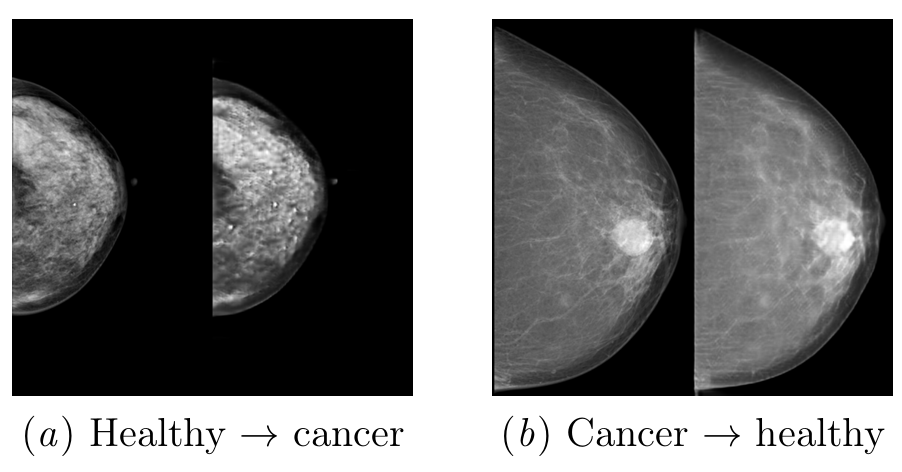
\includegraphics[scale=0.6]{Images/cycle-gan-breast-cancer.png}
    \caption{CycleGAN example -- transforming between breast cancer and healthy sample~\cite{CycleGANBreastCancer}.}
    \label{fig:cycleGANBreastCancer}
\end{figure}

\textbf{Data Augmentation Generative Adversarial Networks (DAGANs)}: DAGANs represent a significant advancement in GAN architecture, specifically aimed at enhancing data augmentation capabilities. Unlike traditional GANs, which generate new data points from random noise, DAGANs augment existing datasets by producing variations of the input data. This is accomplished by incorporating a U-Net-like structure into the generator architecture, enabling it to more accurately capture and reproduce variations within the context of the input data. Additionally, DAGANs implement an augmented adversarial training method technique that enhances the generator's ability to produce diverse, yet plausible, data variations. This makes them particularly useful for applications that require extensive and diverse training data from limited samples, such as one-shot learning.

When it comes to different GANs, \textbf{choosing the appropriate architecture} is crucial and depends on the dataset's specific needs and computational resources. DCGANs, Conditional GANs, StyleGANs, CycleGANs, and DAGANs each offer unique approaches for generating new, realistic data samples that significantly enhance data augmentation efforts. Each GAN type possesses distinctive features, such as managing class imbalances, adjusting particular image features, or converting images across diverse styles without the need for matching examples. Hence, selecting the most suitable GAN architecture requires careful consideration of what specific improvements are required and the computational capabilities available to ensure optimal machine learning model performance.

\begin{figure}[!htb]
    \centering
    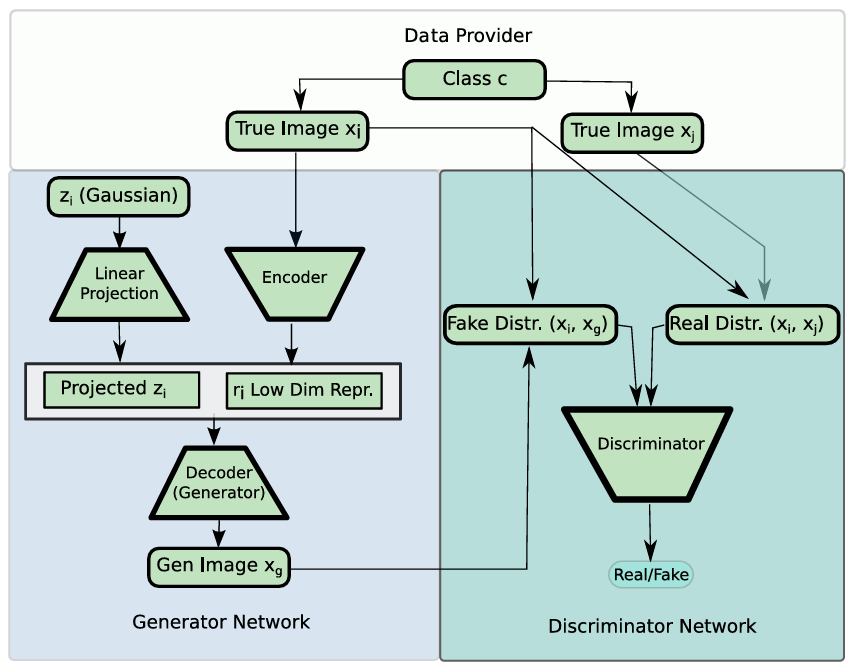
\includegraphics[scale=0.8]{Images/dagan-architecture.png}
    \caption{\textbf{DAGAN Architecture}. The image we want to use for augmentation is projected down to a lower dimensional representation and random noise is concatenated to this signal. This serves as an input to the generator and helps to limit variations of the input image, which is a valuable feature for image augmentation~\cite{DAGANPaper}.}
    \label{fig:DAGANArchitecture}
\end{figure}

%---------------------------------------------------------------------------

\section{Domain Specific Audio Augmentation}
\label{ssec:domainSpecific}

This section of the thesis analyzes the significance of Mel Spectrograms and their role in transforming audio signals into image-based formats for analytical purposes. Various approaches to enhancing raw audio and custom techniques for augmenting spectrogram representations are explored. These methods enhance datasets for training deep learning models in sound analysis.

\subsection{Mel Spectrograms}
\textbf{Mel Spectrograms} are visual representations of audio files created by converting audio signals into the frequency domain using the Short-Time Fourier Transform (STFT). The STFT splits the signal into short segments and computes the Fourier transform for each, resulting in a two-dimensional array representing time and frequency. These frequencies are then converted to the Mel scale, which mimics human pitch perception, using a series of triangular overlapping filters.

Mel Spectrograms allow audio file classification to be treated like image classification, enabling the use of techniques such as convolutional neural networks (CNNs). Advantages of using Mel Spectrograms include:
\begin{itemize}
   \item \textbf{Dimensionality Reduction}: For a 30-second audio file sampled at a frequency of $22,050$ Hz, dimensionality reduction can decrease the number of input parameters by a factor of $10$, from $[1, 661, 500]$ to $[64, 1024]$.
   \item Mel spectrograms map audio signals to a frequency scale that reflects \textbf{human hearing}, making them more relatable and intuitive for tasks involving human sound perception.
   \item Mel spectrograms simplify the \textbf{audio patterns extraction}, aligning with the way CNNs identify patterns in images, allowing for more effective audio recognition.
   \item \textbf{Robustness to noise} and variations.
   \item Enable sound to be analyzed using \textbf{image-processing techniques}.
\end{itemize}

While some augmentations are best applied directly to the raw audio signal, others are more suited to the spectrogram format.  Figure \ref{fig:audioAugDiagram} provides a visualization of this concept.

\begin{figure}[!htb]
    \centering
    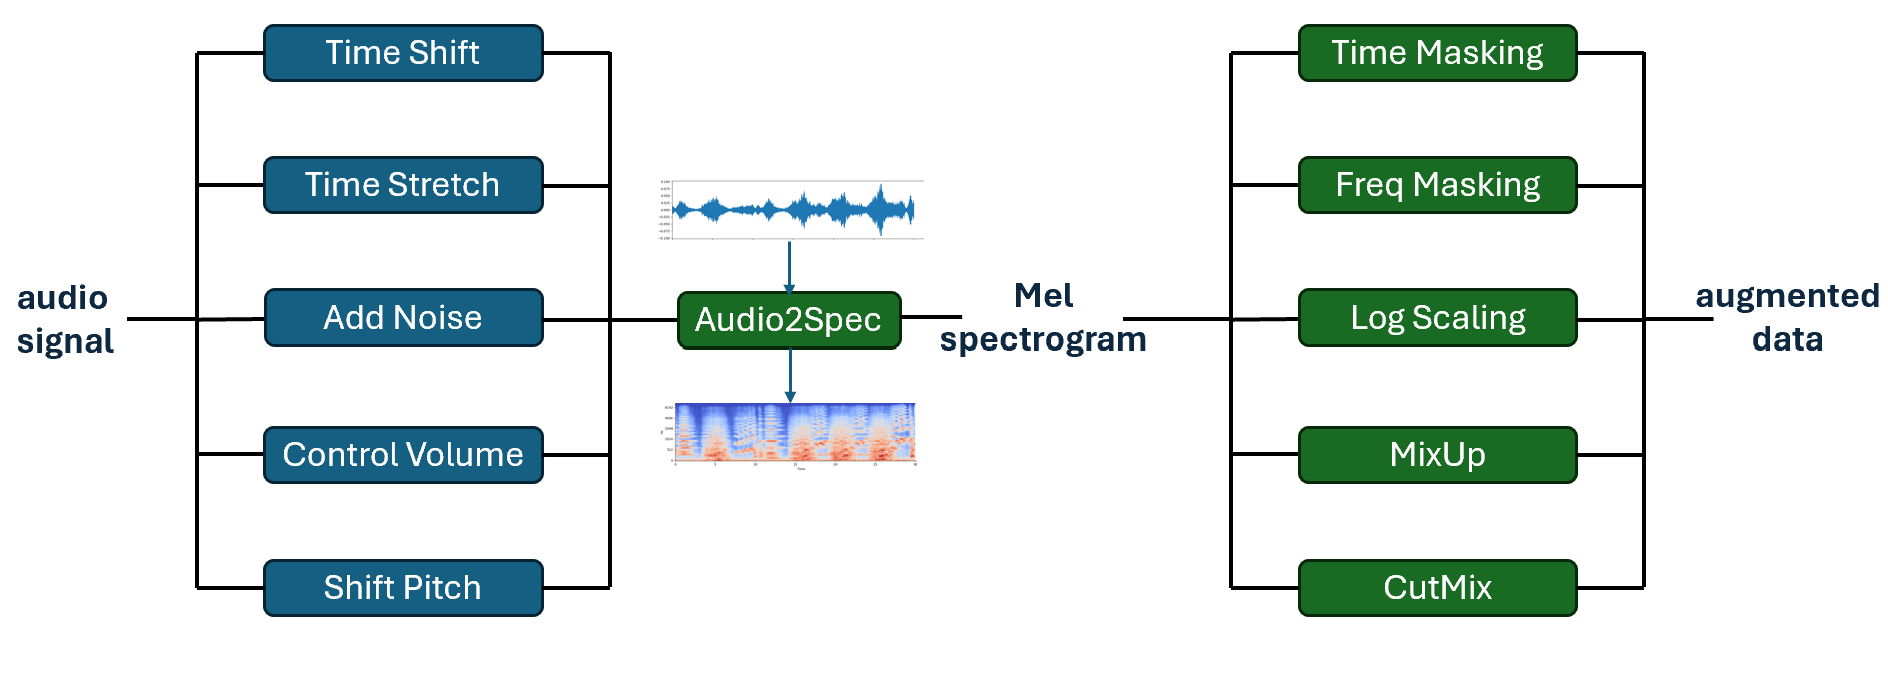
\includegraphics[scale=0.58]{Images/audio-augmentation.png}
    \caption{Audio Augmentation diagram.}
    \label{fig:audioAugDiagram}
\end{figure}

\subsection{Audio Signal Augmentation}

This section of the thesis is based on the article "Data Augmentation and Deep Learning Methods in Sound Classification: A Systematic Review"~\cite{AudioAugmentation}.

\textbf{Time Shifting} is an augmentation technique, where an audio sample is delayed or advanced in time. The utility of this method lies in its ability to simulate the real-world scenario where sounds may not always start at the same temporal threshold, which helps the model handle these events effectively.

\textbf{Time Stretching} manipulates the time dimension of the sound wave without altering its pitch. This technique teaches models that variations in playback speed and duration of audio events can occur. That is particularly beneficial in voice recognition systems where speaker cadences vary widely.

\textbf{Adding Noise} is a universal method in audio augmentation, imitating the presence of ambient noise in everyday soundscapes. By blending signals with a range of noise types, models are trained to extract relevant audio features even when masked by background interference. Test data is often collected in noisier environments, requiring models to effectively manage and adapt to these challenges.

\textbf{Volume Control} serves as another augmentation strategy, which adjusts the amplitude of audio signals. This method teaches models to determine audio patterns across different decibel levels, mitigating the model's sensitivity to volume variations that can affect the clarity of sounds in practical applications.

\textbf{Pitch Shifting} involves changing the pitch of audio signals to mimic the natural pitch variations in human speech and musical instruments. This technique is crucial for models designed for speech-processing tasks and music genre classification, where pitch plays a significant role in conveying meaning.

\begin{figure}[!htb]
    \centering
    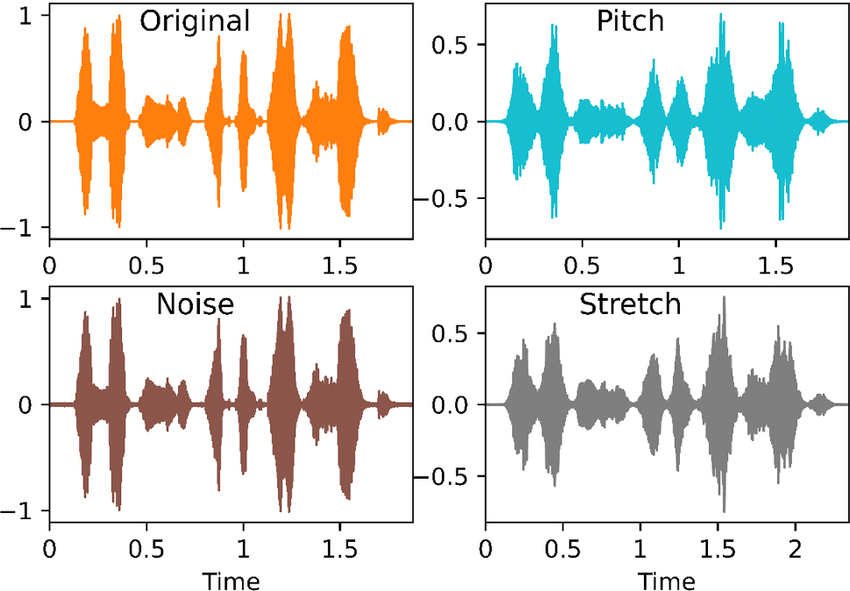
\includegraphics[scale=1.2]{Images/raw-audio-augmentations.png}
    \caption{Audio signal augmentation examples~\cite{RawAudioAugmentation}.}
    \label{fig:rawAudioAugmentation}
\end{figure}

\subsection{Spectrogram Based Augmentation}

The first method is called \textbf{Time Masking}. It involves hiding sequential time steps in the Mel spectrogram, similar to slicing away a vertical strip from an image. This forces learning algorithms to interpolate missing temporal information, improving resilience to temporal distortions, omissions, or differences in real-world audio. The width and number of strips can be adjusted using function parameters.

\textbf{Frequency Masking} is similar to time masking but targets the frequency axis, hiding horizontal stripes to mask a range of frequencies. This simulates frequency loss, crucial for training models to perform well even when certain frequency bands are missing or damaged, a common occurrence in various acoustic environments.


\textbf{Log Scaling}, is another method that involves applying a logarithmic function to the frequency domain. This enhances the detail in lower frequencies and brings the spectrogram's representation closer to human hearing perception.

\textbf{MixUp} in audio blends two different audio clips and their corresponding labels to create a new sample. This process merges the audio signals and computes a weighted average of their labels. For example, combining "people talking" and "guitar playing" clips results in a new audio clip and label reflecting this mix, based on a lambda parameter. This encourages the model to learn from mixed audio scenarios, enhancing its ability to handle uncertainty and overlapping sounds common in real-world conditions.

\textbf{CutMix} in audio slices a segment from one audio spectrogram and pastes it onto another, creating a composite spectrogram. Unlike \textit{MixUp}, which uniformly blends audio, \textit{CutMix} forces the model to make predictions from incomplete or obscured sounds, as the pasted segment may hide key features of the base audio. This technique improves the model's performance in scenarios where parts of a song might suggest a different musical genre than the song as a whole.

\begin{figure}[!htb]
    \centering
    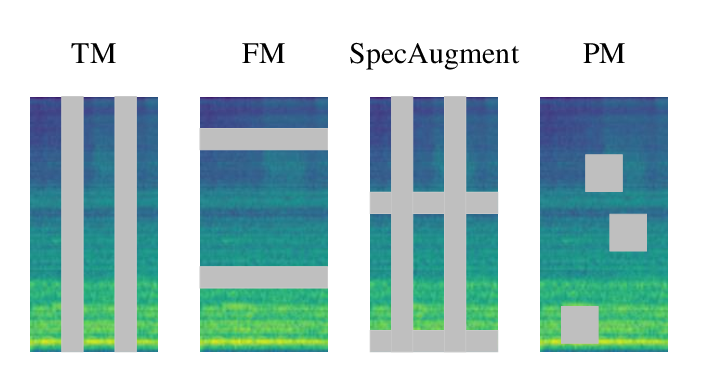
\includegraphics[scale=0.8]{Images/spectrogram-masking.png}
    \caption{Spectrogram-based augmentation example~\cite{MaskingAugmentation}.}
    \label{fig:specAudioAugmentation}
\end{figure}

\section{Data Augmentation Safety}

In the context of data augmentation techniques, it is essential to recognize both their benefits and potential drawbacks to ensure that they improve model performance instead of undermining it. This section of the thesis considers the risks associated with various common augmentation strategies and highlights the importance of careful implementation.

\textbf{Rotation} and \textbf{flipping} are widely used for augmenting image data. However, these methods can introduce significant distortions if not appropriately applied. For instance, arbitrary rotation of images such as flowers can lead a model to learn incorrect orientations since flowers in nature do not exhibit a full 360-degree rotational symmetry. Similarly, horizontally flipping text data can create nonsensical sequences, making it challenging to analyze documents with natural language processing.

\textbf{Cropping} and \textbf{shifting} are another commonly employed techniques that, while useful in focusing a model's attention on salient image features, can also remove essential parts of an image. In scenarios where important features are cropped out, the model may learn from incomplete or irrelevant data, leading to poor performance. This is particularly critical in applications like facial recognition, where missing features such as eyes or mouths can severely impact the model's accuracy.

The use of \textbf{Generative Adversarial Networks} (GANs) introduces a different set of challenges. While GANs are powerful in generating new, synthetic images, they can produce data that does not represent any real-world distribution if not carefully tuned. This can lead to models that perform well on synthetic data but poorly on actual data.

\textbf{Mixing images} can also lead to confusion. If only a small, yet crucial, part of an image is used and overlaid by a less relevant part of another image, it can mislead the model about the importance and context of the features.

In the field of \textbf{medical image analysis}, improper geometric or color transformations can distort anatomical details and critical color information, potentially leading to incorrect diagnoses. For example, overly darkening an image can obscure important details, while removing red can hide signs of bleeding.

These examples highlight the need for careful planning and evaluation when implementing data augmentation techniques. It is crucial to understand the specific characteristics and requirements of the data to ensure that augmentation methods are enhancing the training process and not introducing misleading biases. Such considerations are vital for developing robust machine learning models that are reliable and effective in real-world applications.
	\chapter{Methodolodgy}
\label{cha:Methodology}

%---------------------------------------------------------------------------
\section{Programming Environment}
\label{sec:programmingEnv}
Machine learning and data analysis projects are often executed using Jupyter notebooks. This study also utilized them due to their compatibility with Python, a language with extensive neural network training and result visualization libraries. Jupyter Notebooks seamlessly integrate Python code with explanatory comments and visualizations, facilitating well-documented work. The primary reason for selecting Jupyter Notebooks was their compatibility with Google Colab and Kaggle Notebooks, which provide free GPU resources. Utilizing GPUs significantly reduced network training time, enabling the evaluation of a much larger array of architectures and scenarios.

As previously mentioned, the technical part of the master thesis was conducted using the \textit{Python} programming language. Diagram \ref{fig:pythonLibraries} illustrates the libraries used. The specific versions of the libraries are included in the code.

\begin{figure}[!htb]
    \centering
    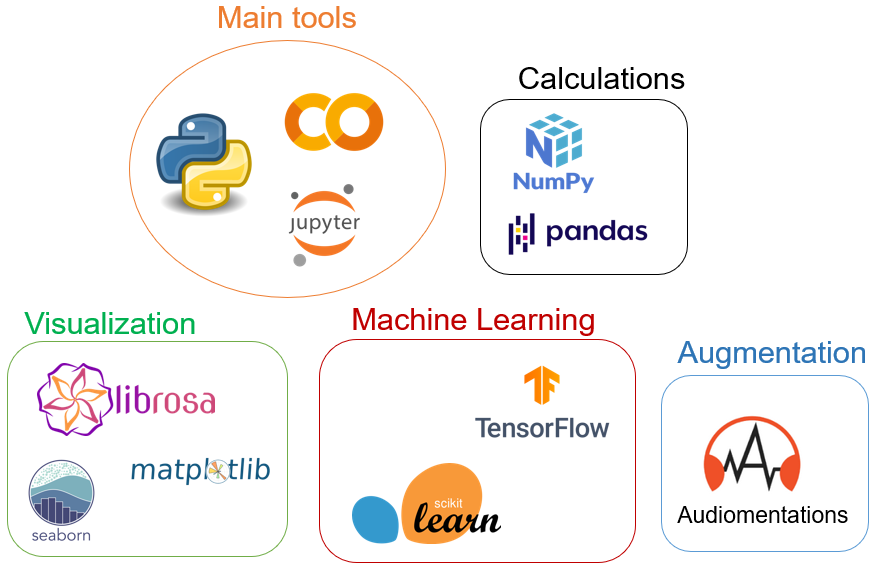
\includegraphics[scale=0.55]{Images/python-libraries.png}
    \caption{Programming language and libraries used in this thesis.}
    \label{fig:pythonLibraries}
\end{figure}

\section{Description of Datasets}
\label{sec:datasets}

To compare augmentation methods, various datasets were used to ensure more generalizable results. One dataset was selected for its typical and general characteristics, serving as a baseline. Another dataset was designed for one-shot learning, containing minimal data per class. The third dataset evaluated image augmentation in a domain-specific application, using audio files that are treated similarly to images.

%---------------------------------------------------------------------------

\subsection{Flowers 102 Dataset}
\label{ssec:Flowers102Dataset}

The Flowers $102$ dataset~\cite{Flowers102} consists of $8,189$ images, each depicting one of 102 different flower categories commonly found in the United Kingdom. Each category corresponds to a single species such as daisies, tulips, roses, and many others. The number of images per class varies, but each class is represented with at least $40$ images, which helps in training robust models.

\begin{figure}[!htb]
    \centering
    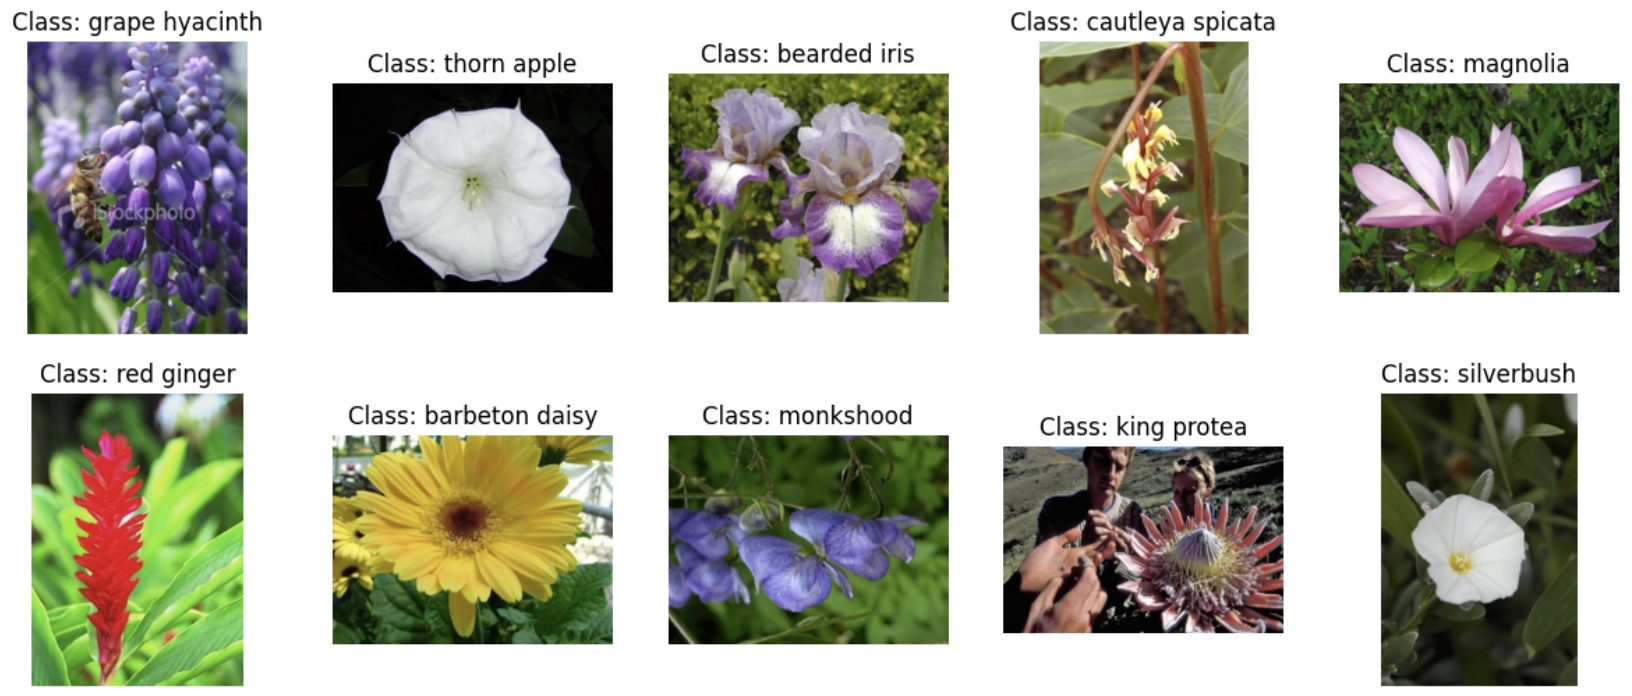
\includegraphics[scale=0.7]{Images/flowers-example.png}
    \caption{Samples from Flowers 102 dataset.}
    \label{fig:flowersExample}
\end{figure}

The Flowers 102 dataset is widely utilized for training and evaluating deep-learning models that specialize in image classification. Such models require exceptional recognition capabilities to distinguish between closely related species of flowers. As a standard dataset, it is highly respected in academic research for testing novel approaches in computer vision, machine learning, and especially in transfer learning, where pre-trained models are adapted to this dataset to achieve superior specificity. The dataset is frequently referenced in research papers and leveraged in diverse machine-learning competitions and educational initiatives to evaluate algorithm effectiveness.

One key challenge the Flowers 102 dataset poses is the intra-class variation and inter-class similarity. Some flower species in the dataset have considerable variation in appearance due to different growth conditions and developmental stages, while different species may look quite similar to each other. Shape isomap is shown in Figure \ref{fig:shapeIsomap}.

\begin{figure}[!htb]
    \centering
    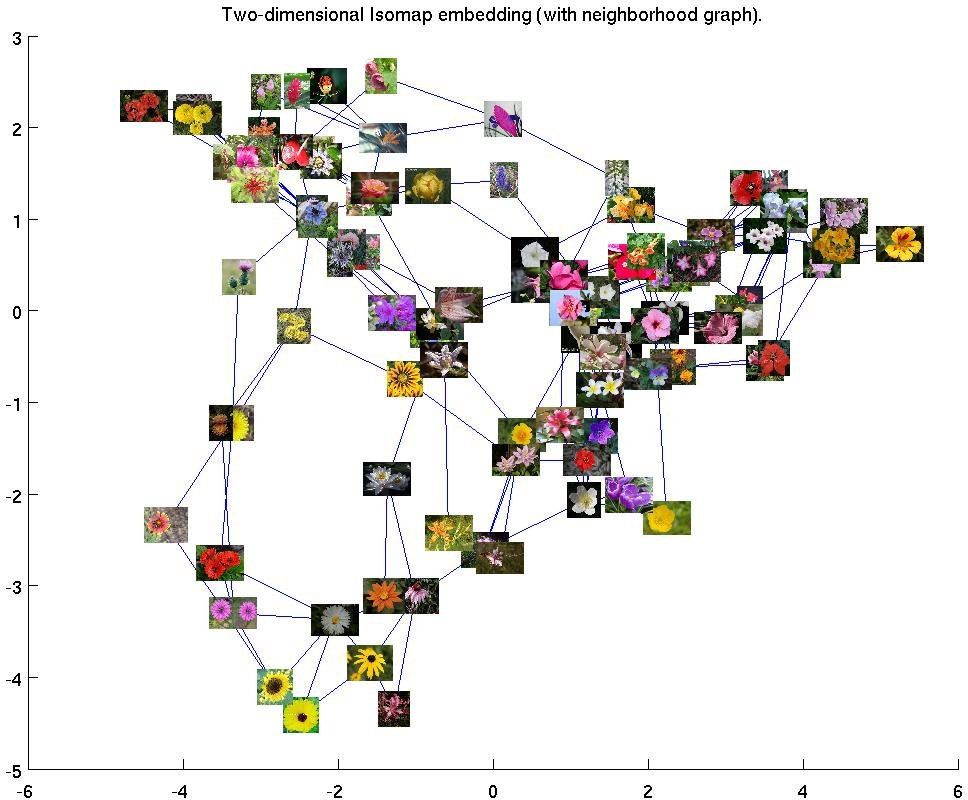
\includegraphics[scale=0.3]{Images/shape-iso.jpg}
    \caption{Shape isomap of Flowers 102 dataset~\cite{Flowers102}.}
    \label{fig:shapeIsomap}
\end{figure}

%---------------------------------------------------------------------------

\subsection{One-shot Flowers 102 Dataset}
\label{ssec:flowersOneShotDataset}

To tackle the difficulties of one-shot learning, smaller datasets were created based on "Flowers 102"~\cite{Flowers102}. Specifically, \textbf{5, 10 or 20 images were selected at random from each of the 102 flower categories} to investigate the efficiency of data augmentation techniques under these conditions. With a limited number of images per class, the risk of overfitting and the need for the model to generalize from a small set of examples are significant challenges. However, by implementing data augmentation techniques, it should be possible to improve the model's performance significantly. 



%---------------------------------------------------------------------------

\subsection{GTZAN Dataset}
\label{ssec:gtzanDataset}

The GTZAN dataset~\cite{GTZAN} is one of the pioneering collections for music genre classification, comprising a total of 1,000 audio tracks each lasting 30 seconds. The dataset is evenly distributed across 10~different genres, including blues, classical, country, disco, hip-hop, jazz, metal, pop, reggae, and rock, with each genre represented by 100 tracks. This uniform distribution aids in creating balanced classification models.

\begin{figure}[!htb]
    \centering
    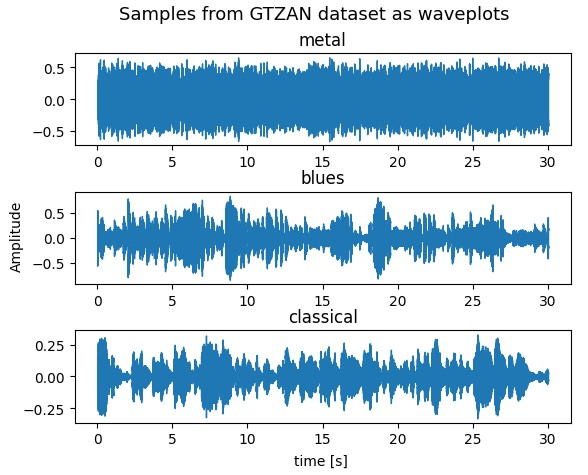
\includegraphics[scale=0.6]{Images/gtzan-example.jpg}
    \caption{Samples from GTZAN dataset~\cite{GTZAN} visualized as waveforms.}
    \label{fig:gtzanExample}
\end{figure}

Widely used in evaluating machine learning models for music analysis, the GTZAN dataset has become a benchmark in the field. It allows researchers to test and demonstrate the efficiency of various audio processing techniques and algorithms to understand and categorize musical styles. Models trained on the GTZAN dataset often employ techniques like Fourier transforms to capture frequency components and machine learning algorithms such as k-nearest neighbors, decision trees, and neural networks to classify audio samples.

In this research, the GTZAN dataset was utilized to explore the impact of data augmentation techniques on \textbf{domain-specific} data. Methods such as time stretching, pitch shifting, and adding background noise were implemented to investigate how these augmentations could enhance the robustness of genre classification models. The focus was on addressing overfitting and improving model generalizability across varied musical inputs.

A notable challenge when working with the GTZAN dataset involves handling the diversity within each genre and the potential overlap between different genres, where certain tracks might share characteristics typical of multiple genres. Another issue is the quality and encoding of the audio tracks, which can affect the performance and generalization capability of the trained models. Additionally, to utilize this dataset with traditional image classification methods, it is necessary to convert the data into MEL Spectrograms. 

In academic circles, the dataset is frequently cited for illustrating the capabilities and limitations of computational approaches to music genre recognition. This is another reason why this dataset was chosen.

%---------------------------------------------------------------------------

\section{Data Preprocessing and Augmentation}

\subsection{Steps common for all datasets}
\label{ssec:commonProcessing}

The initial datasets were loaded and categorized following the existing directory structure to ensure \textbf{consistent data organization}. This systematic arrangement allowed for an intuitive mapping between the data categories and their respective labels.

A \textbf{seed} was set at the beginning of the process for \textbf{NumPy}, \textbf{TensorFlow}, and the \textbf{random} package to ensure repeatability across multiple experimental runs. This is crucial for accurate reproduction and comparison of results, which is essential when evaluating the efficacy of various models and experiments.

Subsequently, the data was divided into \textbf{training, validation, and test sets} in approximate proportions of 70\%, 20\%, and 10\%, respectively. The split was chosen to facilitate optimal training of neural networks while maintaining an adequate validation and testing set. The division was stratified, which means that it was arranged in a way that ensures an even distribution of classes in all sets. Cross-validation was not utilized due to the significant computational time required for training neural networks in each fold.


The \textbf{labels were encoded using one-hot encoding} to facilitate their use in training neural networks. This encoding method transforms categorical labels into a binary matrix, where each column corresponds to a unique class. One-hot encoding ensures compatibility with the network's output layer and simplifies the representation of categorical data. Additionally, this encoding approach enables the application of data augmentation techniques such as \textit{MixUp} and \textit{CutMix}.

The images were then grouped into \textbf{batches} containing 32 examples each to streamline the training process. The number of \textbf{epochs} was carefully chosen to balance training time and model performance, ensuring that the networks had sufficient time to learn from the data without overfitting.

Regarding data augmentation, it could be \textbf{turned on or off} for each experiment to assess its impact. The \textbf{probability of augmentation} occurring was configurable separately for traditional techniques, \textit{MixUp}, \textit{CutMix}, and others, allowing fine-tuning of the augmentation process for the specific characteristics of each problem. This flexibility ensured that the augmentation strategy was optimized to address the challenges of the dataset and improve model performance accordingly.

\textbf{TensorFlow datasets} which defined processing and augmentation steps were built for each dataset used in the experiments. As the preprocessing and dataset preparation varied between datasets, the specific details for each will be described separately in the following sections.

\subsection{Flowers 102}
\label{ssec:Flowers102Processing}

In the processing and augmenting of the Flowers 102 dataset, a series of steps were implemented to strengthen the training data. The images were \textbf{flipped horizontally} to mimic the natural left-right growth patterns of flowers, while \textbf{brightness} and \textbf{contrast} modifications simulated the diverse lighting environments existing in nature. A \textbf{Gaussian filter} was utilized to replicate natural blurring and noise.

The images were \textbf{rotated up to 45 degrees} in either direction, as flowers typically do not grow at extreme angles. The noise was injected to reflect environmental disturbances and camera sensor noise. \textbf{Random cropping} was applied to emulate zooming, which helped the model identify flowers from varying distances.

The process of augmentation was carried out based on the probabilities mentioned in the previous section. After these adjustments, all images were \textbf{resized to 224 x 224 pixels} to comply with the standard input dimensions of \textit{ResNet} and \textit{EfficientNet}. \textit{MixUp} and \textit{CutMix} were also used across batches to enrich the dataset and boost the model's generalization capacity.

\begin{figure}[!htb]
    \centering
    \begin{subfigure}{0.7\textwidth}
        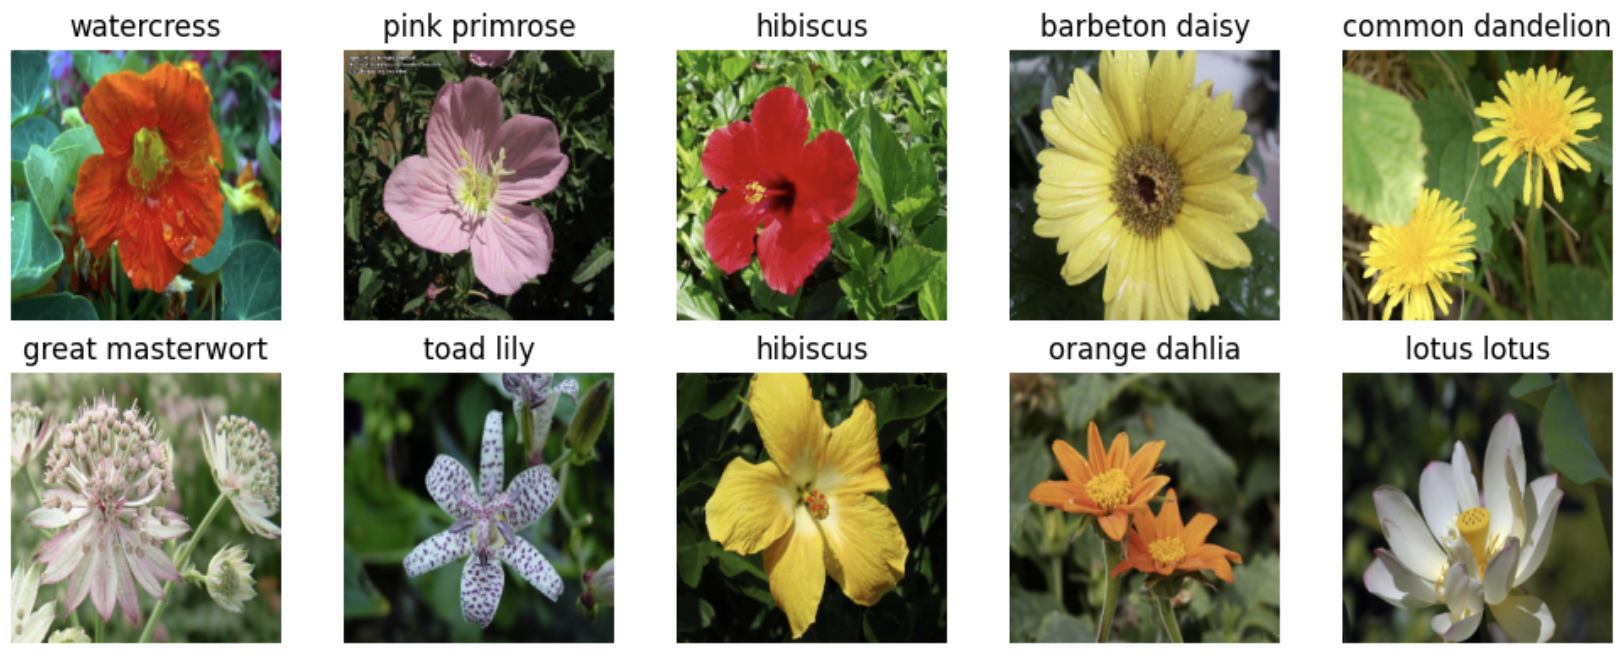
\includegraphics[scale=0.50]{Images/no-augmentation.png}
        \caption{No Augmentation}
    \end{subfigure}
    \vspace{0.3cm}

    \begin{subfigure}{0.7\textwidth}
        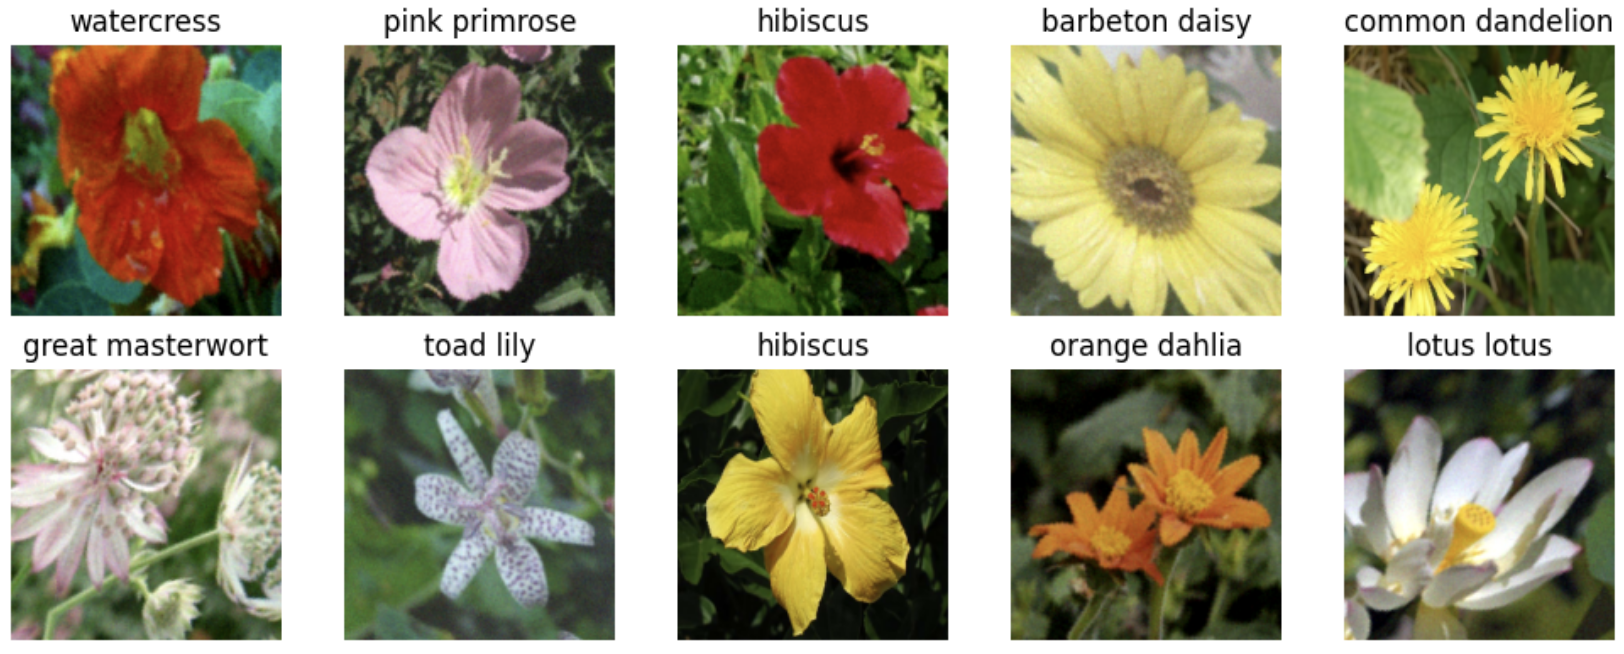
\includegraphics[scale=0.50]{Images/traditional-augmentation-4.png}
        \caption{Traditional Augmentation}
    \end{subfigure}
    \vspace{0.3cm}

    \begin{subfigure}{0.7\textwidth}
        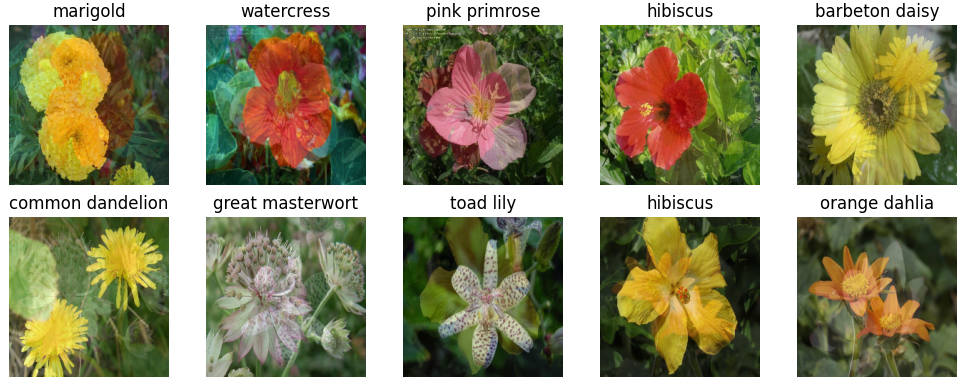
\includegraphics[scale=0.85]{mixup-augmentation.png}
        \caption{\textit{MixUp} Augmentation}
    \end{subfigure}
    \vspace{0.3cm}

    \begin{subfigure}{0.7\textwidth}
        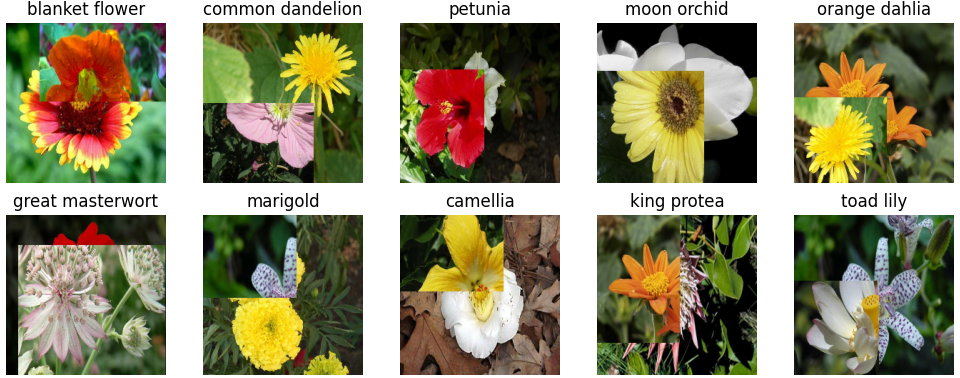
\includegraphics[scale=0.85]{cutmix-augmentation.png}
        \caption{\textit{CutMix} Augmentation}
    \end{subfigure}

    \caption{Augmentations applied to Flowers 102 and One-shot Flowers 102 Datasets. (Source: a) \cite{Flowers102}, b-d) the images augmented with own implementation.)}
    \label{fig:flowersAugmentations}
\end{figure}

As illustrated in Figure \ref{fig:flowersAugmentations}, multiple augmentations can occur simultaneously. For instance, in the image (b), the \textit{Barbeton daisy} flower was rotated, zoomed, and adjusted for contrast at the same time. However, \textit{Hibiscus} flower was not changed at all. It ensures that in each epoch different images are affected and variability of data achieved by augmentation is higher. 

In image (c) we can see \textit{MixUp} augmentation, which impacts both images and labels. For instance, if 30\% of the first image and 70\% of the second image are combined, their corresponding one-hot encoded values will be adjusted to 0.3 and 0.7, respectively. Similarly, in image (d), the \textit{CutMix} augmentation modifies the image and labels based on the visible area. These augmentations can also be combined concurrently, enabling higher data variability and model generalization.

\subsection{One-shot Flowers 102}
\label{ssec:flowersOneShotProcessing}

Processing steps were the same as those described in the previous section except that at the beginning, as mentioned in section \ref{ssec:Flowers102Dataset}, the number of data samples per category was \textbf{restricted to 5, 10, and 20} to explore data augmentation effectiveness in a setting with limited data. The number of epochs was adjusted -- for a smaller amount of examples, more epochs were needed to learn valuable features for validation data classification. If the number of examples in the original dataset was smaller than the restriction threshold, examples were randomly repeated for some classes. 

Since the goal was to train the model under conditions with limited data,  the \textbf{validation set} was extracted from the training set, further reducing the number of training cases below the desired threshold. The \textbf{test set} remained unchanged from the full Flowers 102 dataset to ensure a valid comparison.

\subsection{GTZAN}
\label{ssec:gtzanProcessing}

In addition to the general techniques outlined in section \ref{ssec:commonProcessing}, specific steps were applied to the GTZAN dataset for image augmentation. The original files in the dataset, which have a \textbf{*.wav extension}, required transformation into a format suitable for visual processing. To achieve this, audio files were converted into Mel Spectrograms. Figure \ref{fig:waveSpecExample} shows an illustrative example of the classical music data before and after the transformation from a wave into spectrogram form.

\begin{figure}[!htb]
    \centering
    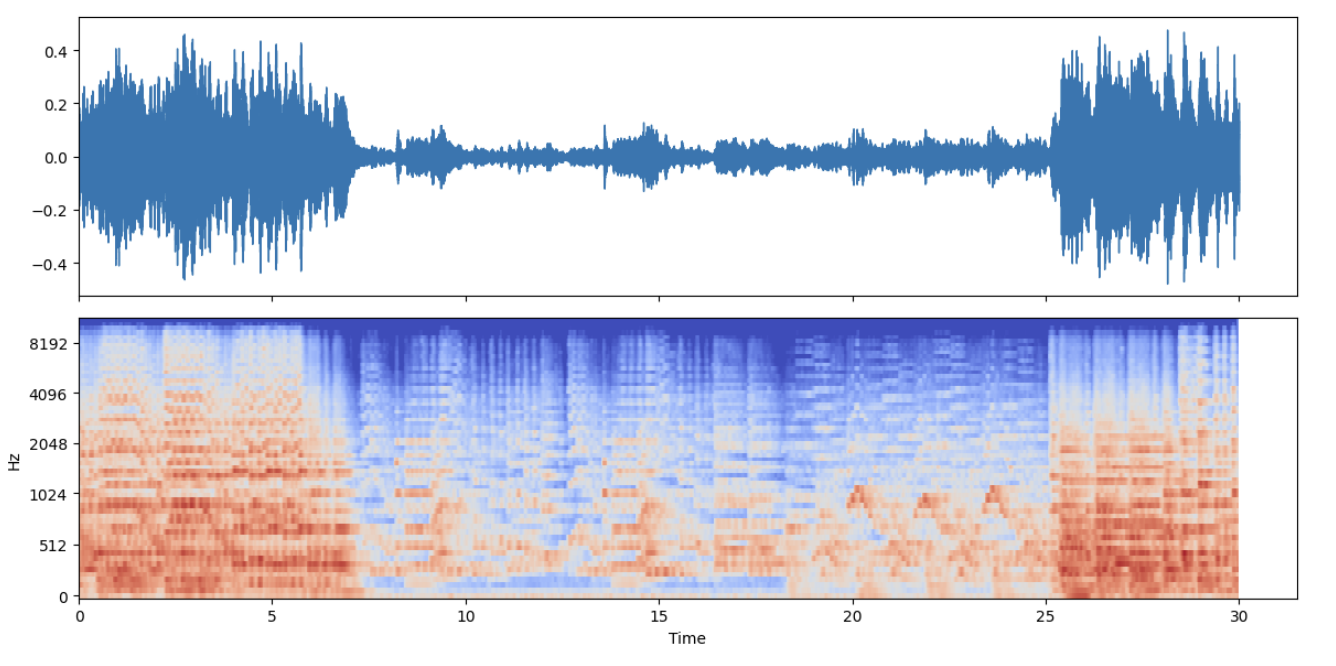
\includegraphics[scale=0.7]{Images/wave-spec-classical.png}
    \caption{Waveform and Spectrogram of classical music. Source:~\cite{GTZAN}.}
    \label{fig:waveSpecExample}
\end{figure}

Parameters of the Short-Time Fourier Transform (STFT) used for this transformation are detailed in the Table \ref{tab:parameters}.
These parameters were chosen based on the literature as detailed in~\cite{GTZANParameters}. The transformation process, implemented in Python's Librosa library, was essential for visualizing and augmenting the data within the framework of image processing techniques, which is the main focus of this thesis.

\begin{table}[h!]
\centering
\caption{Mel Spectrogram parameters.}
\begin{tabular}{|>{}l|l|}
\hline
\textbf{Parameters}    & \textbf{Values}  \\ \hline
Window size            & 1024    \\ \hline
Hop length             & 512     \\ \hline
Number of FFT points   & 4096    \\ \hline
Number of MEL bands    & 64      \\ \hline
Minimum frequency      & 0 Hz    \\ \hline
Maximum frequency      & 8000 Hz \\ \hline
Normalization          & True    \\ \hline
\end{tabular}
\label{tab:parameters}
\end{table}

Moreover, at the waveform level, cropping or padding was used to standardize the length of all audio files before feeding them into the network. Additionally, time shifting and stretching, pitch shifting, and Gaussian noise were incorporated to enhance variability in the training data.

Time and frequency masking were applied after the waveforms were converted into spectrograms. The number and width of the masked strips were adjustable. Furthermore, \textit{MixUp} was applied to the spectrograms using a similar approach as described in previous sections. During training, all types of augmentation were randomly combined using independent probabilities of occurrence. All augmentation types applied to the GTZAN dataset are visualized in Figure \ref{fig:GTZANAugmentations}.

\begin{figure}[!htb]
    \centering
    \begin{subfigure}{0.9\textwidth}
        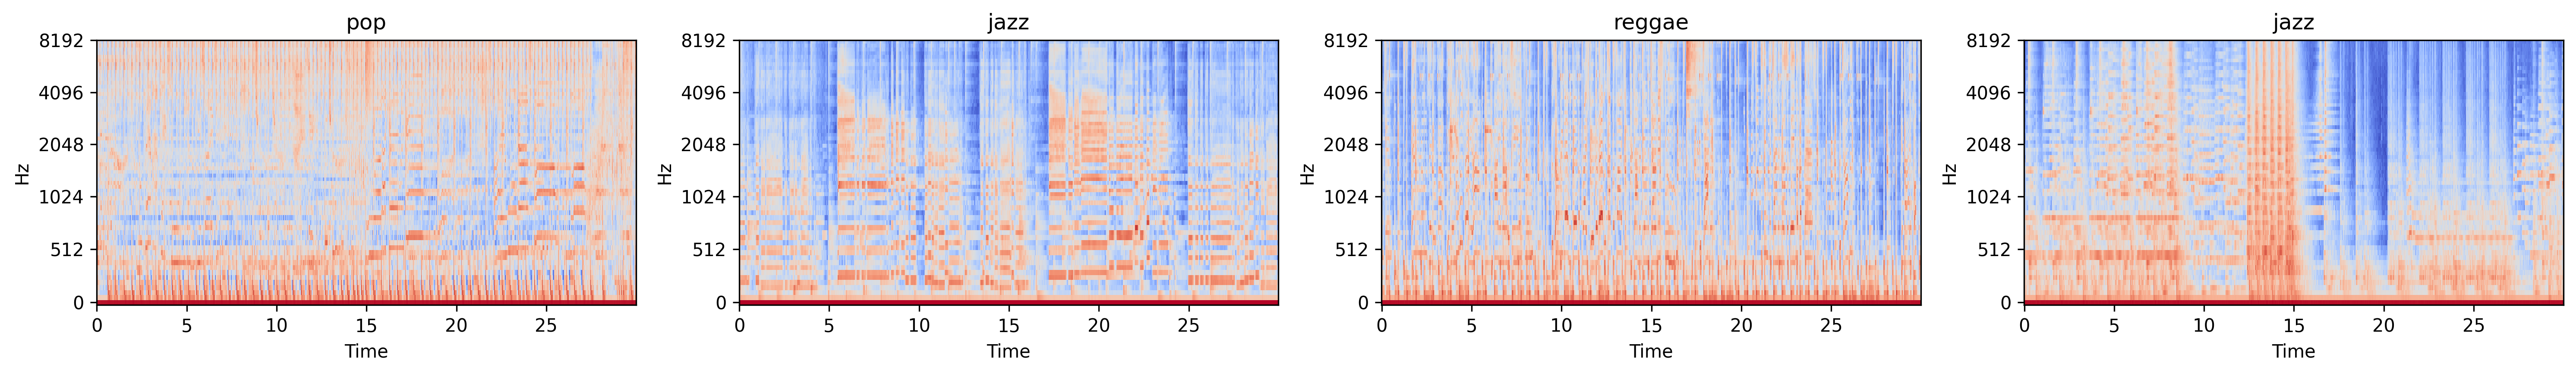
\includegraphics[scale=0.28]{Images/gtzan_new/no_augmentation.png}
        \caption{No Augmentation}
    \end{subfigure}
    \vspace{0.3cm}

    \begin{subfigure}{0.9\textwidth}
        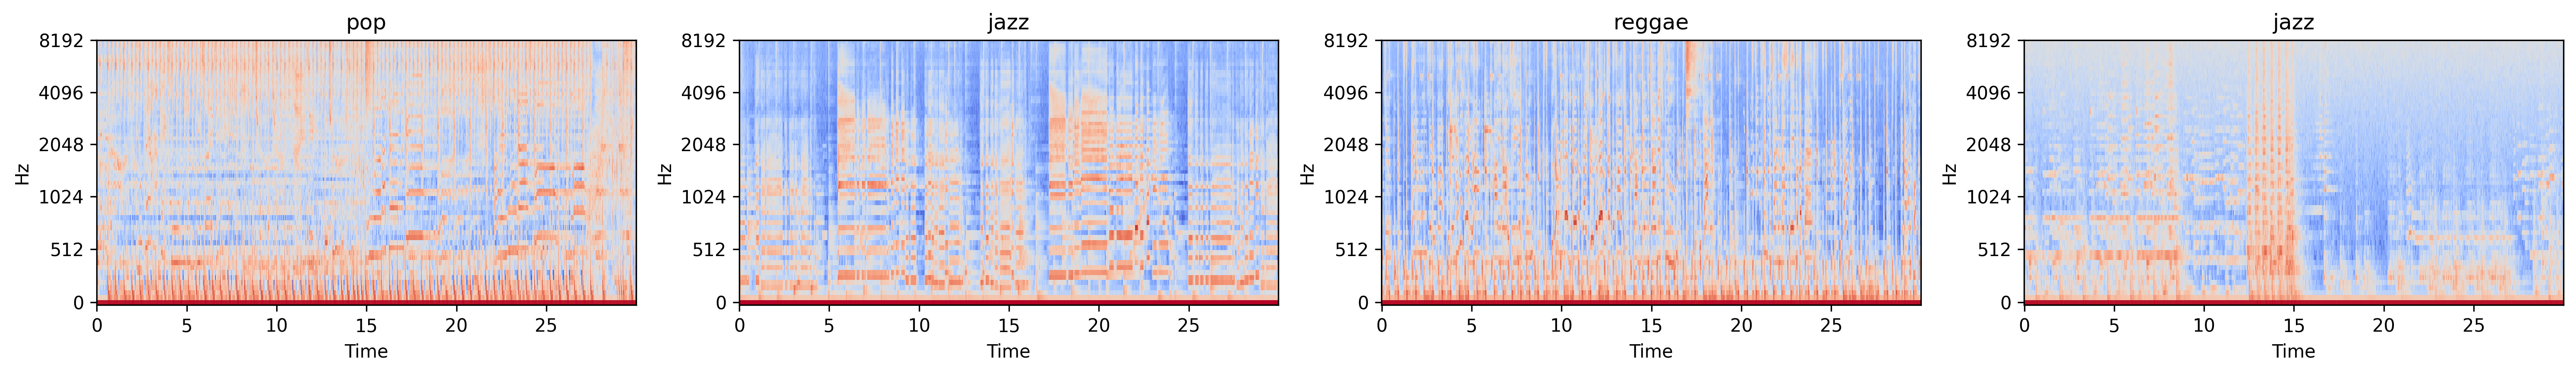
\includegraphics[scale=0.28]{Images/gtzan_new/gn_augmentation.png}\
        \caption{Gaussian Noise}
    \end{subfigure}
    \vspace{0.3cm}

    \begin{subfigure}{0.9\textwidth}
        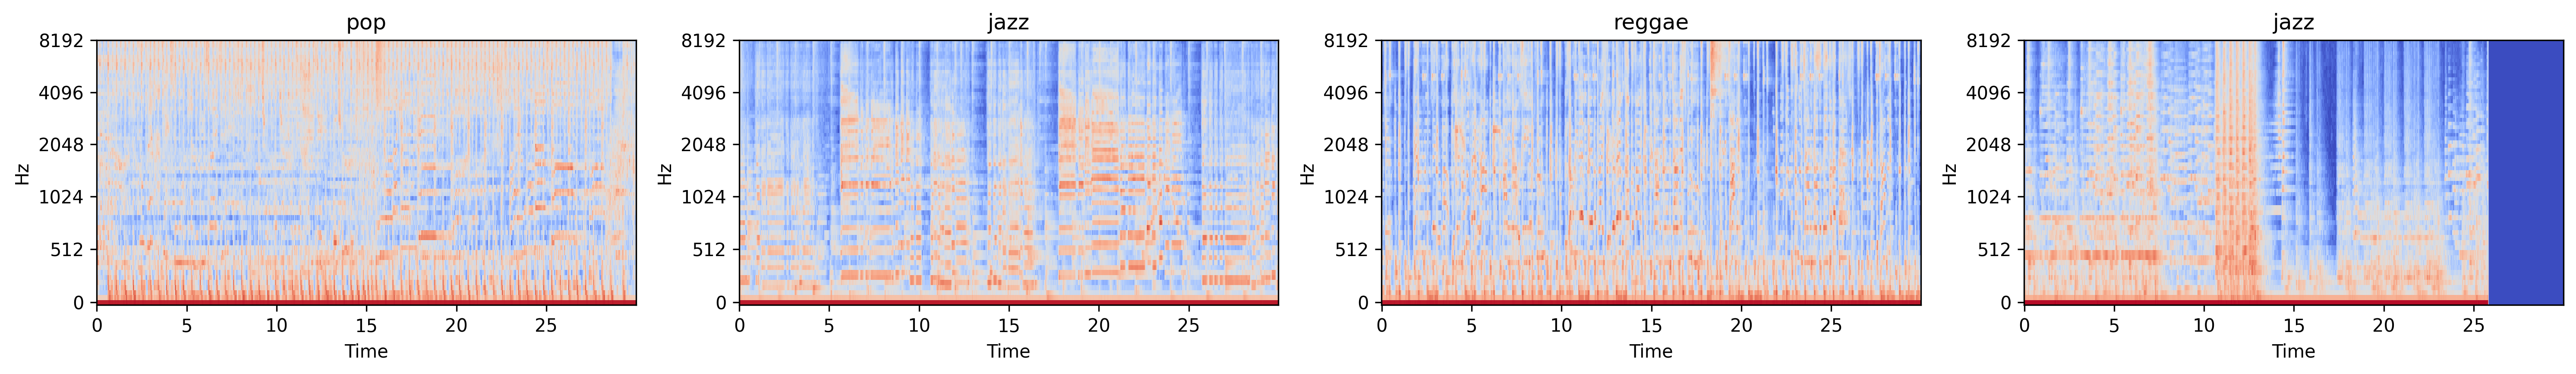
\includegraphics[scale=0.28]{Images/gtzan_new/speedchange_augmentation.png}
        \caption{Speed Change}
    \end{subfigure}
    \vspace{0.3cm}

    \begin{subfigure}{0.9\textwidth}
        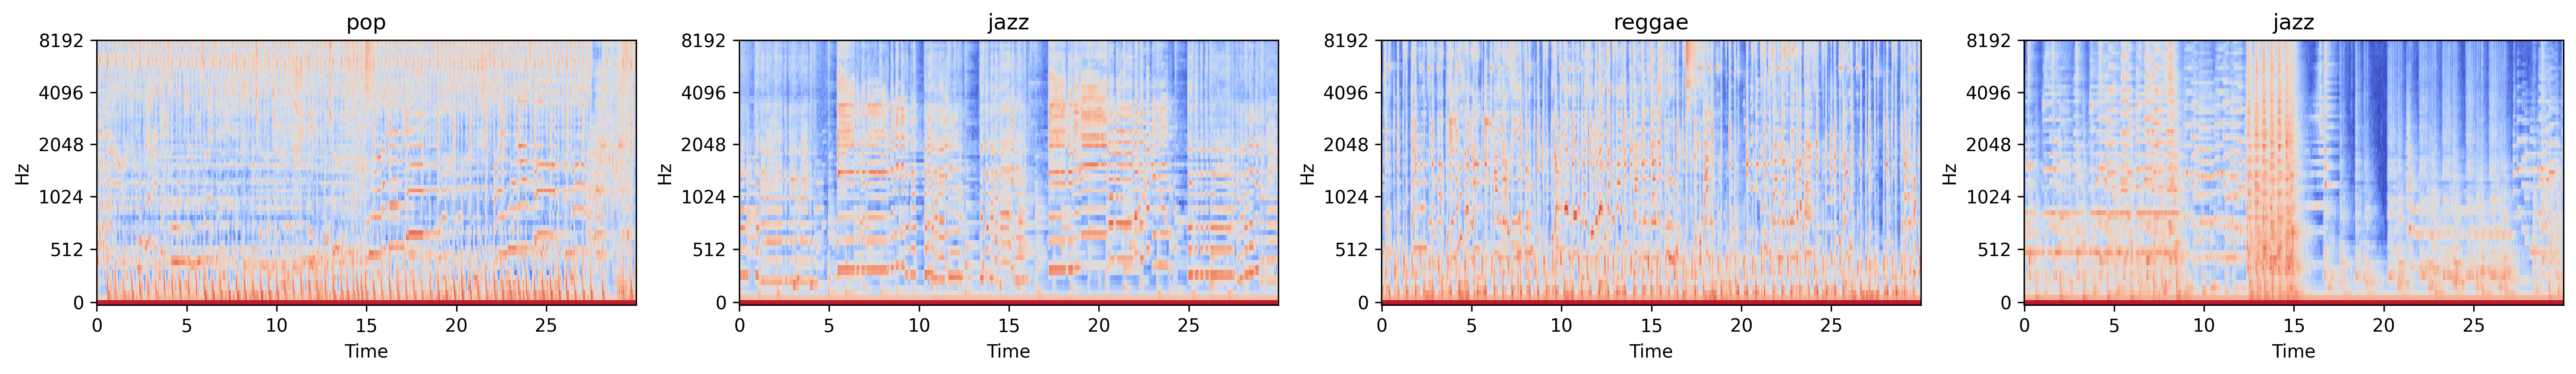
\includegraphics[scale=0.28]{Images/gtzan_new/pitchshift_augmentation.png}
        \caption{Pitch Shift}
    \end{subfigure}

    \begin{subfigure}{0.9\textwidth}
        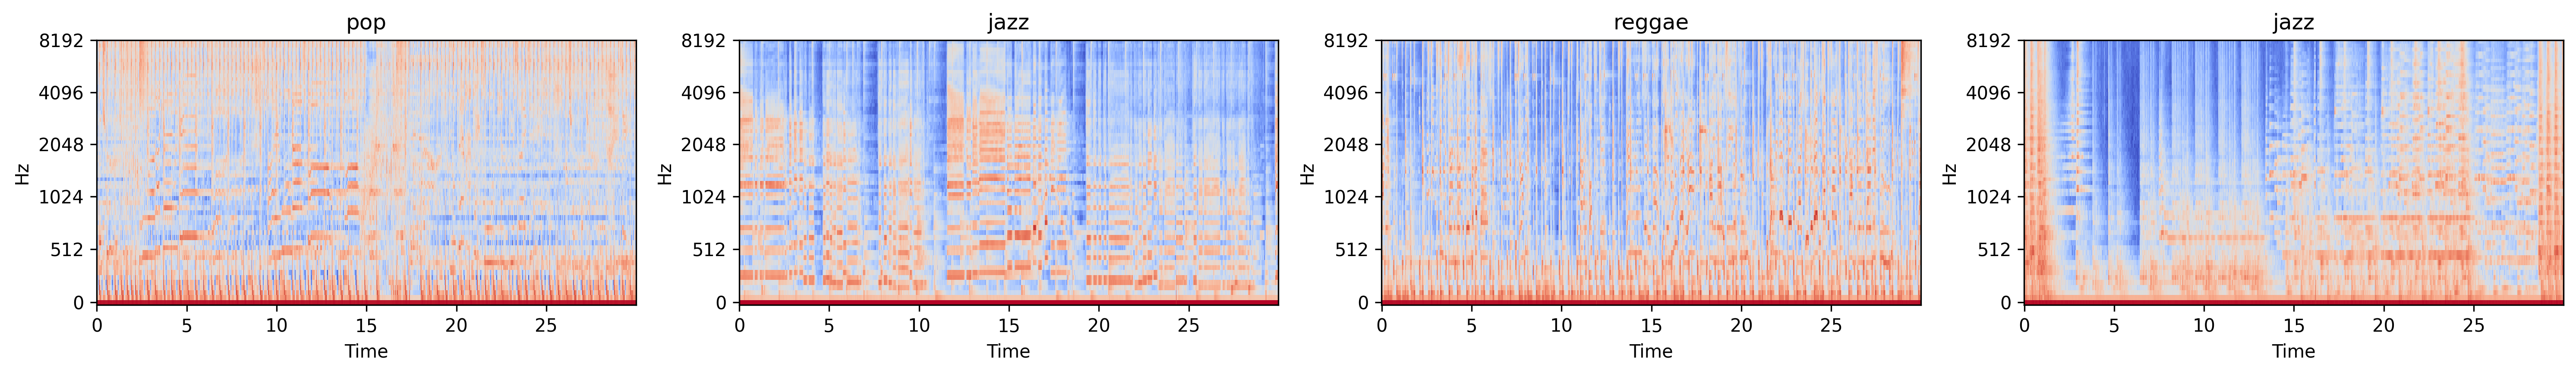
\includegraphics[scale=0.28]{Images/gtzan_new/time_shift_augmentation.png}
        \caption{Time Shift}
    \end{subfigure}

    \begin{subfigure}{0.9\textwidth}
        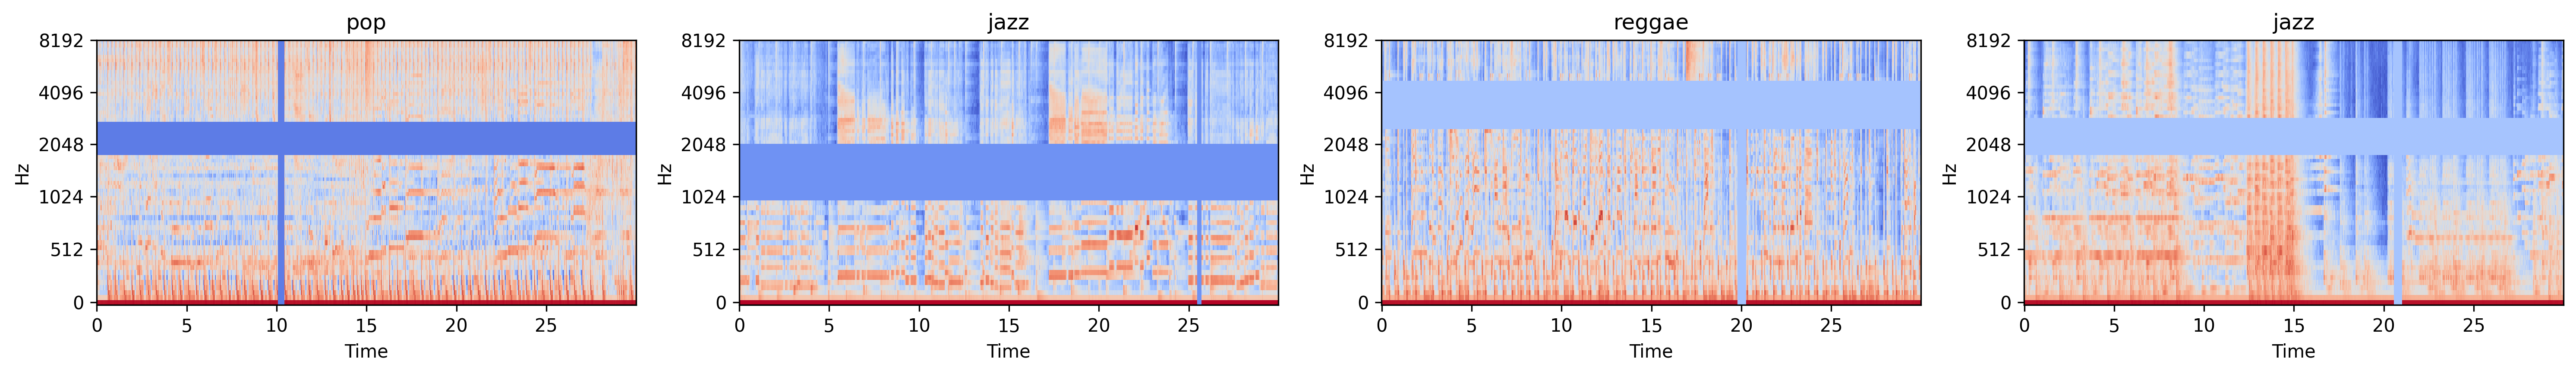
\includegraphics[scale=0.28]{Images/gtzan_new/masking_augmentation.png}
        \caption{Masking Augmentation}
    \end{subfigure}

    \begin{subfigure}{0.9\textwidth}
        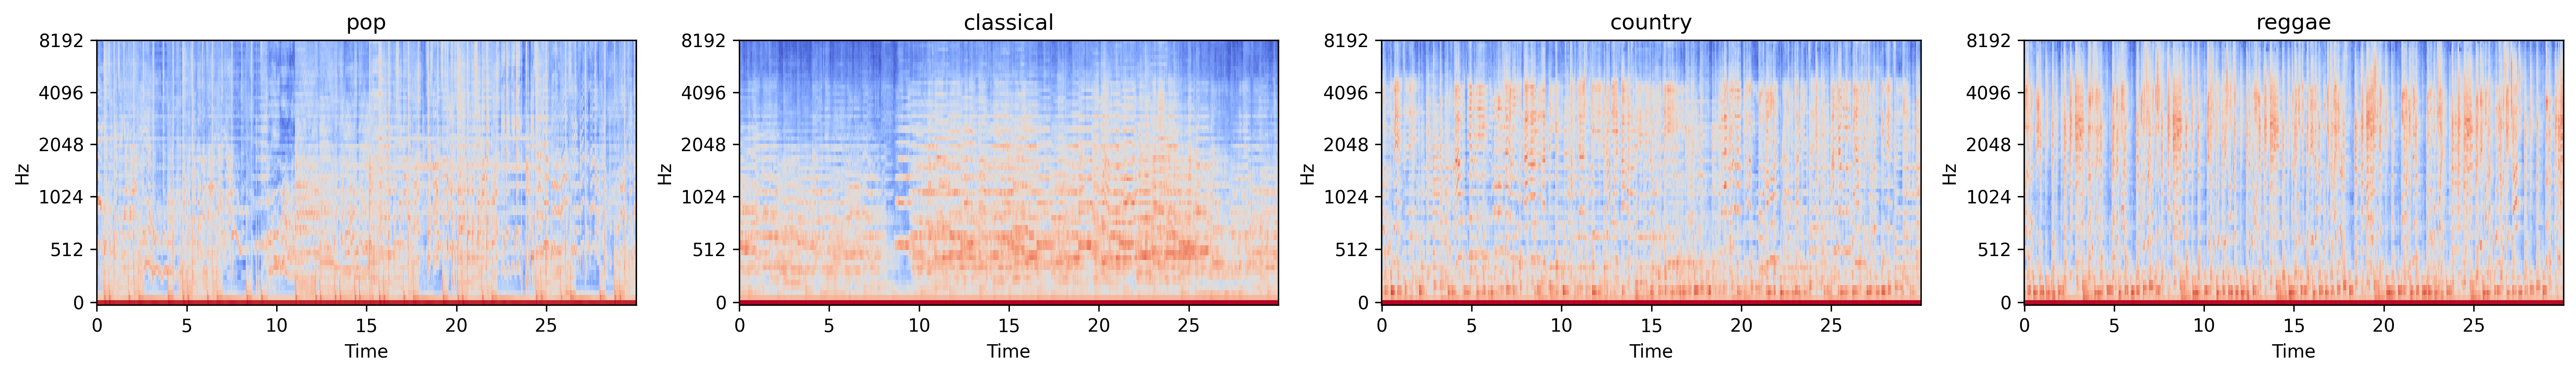
\includegraphics[scale=0.28]{Images/gtzan_mixup_augmentation.png}
        \caption{\textit{MixUp} Augmentation}
    \end{subfigure}

    \caption{Augmentations applied to GTZAN Dataset. Source: a) \cite{GTZAN}, b-g) the images augmented with own implementation.}
    \label{fig:GTZANAugmentations}
\end{figure}



%---------------------------------------------------------------------------

\section{CNN Architectures Used}

In this section, the model architectures used in the experiments are described, specifically \textit{ResNet50}, \textit{EfficientNetB0}, and \textit{EfficientNetB4}. Each model was constructed with appropriate modifications to suit the task, leveraging the principles of transfer learning discussed in previous chapters.

\textbf{ResNet50:} For the ResNet50 model, the base architecture was loaded without the top classification layers using pre-trained weights from ImageNet. All layers were set to trainable to enable fine-tuning. Custom layers were added on top of the base model, including a Global Average Pooling layer followed by a Dense layer with a softmax activation function for classification. The model was then compiled with an appropriate optimizer, loss function, and evaluation metrics.

\textbf{EfficientNetB0, EfficientNetB4}:  The EfficientNet model followed a similar approach. The base EfficientNet architecture was loaded without the top layers, and pre-trained weights from ImageNet were utilized. An input layer was defined, and the base model was applied to this input. A Global Average Pooling layer was added, followed by a Dense layer with 32 neurons, batch normalization, and dropout for regularization. The final Dense layer used a softmax activation function for classification. The model was compiled with the necessary components for training.

In case of the GTZAN dataset, the input shape was $64 x 1292$, which is different from the default one. The number of parameters for each network is shown in Table \ref{tab:modelParameters}.
\begin{table}[h]
    \centering
    \caption{Comparison of Model Parameters.}
    \begin{tabular}{|c|c|c|}
        \hline
        \textbf{Model} & \textbf{All Parameters} & \textbf{Trainable Parameters} \\
        \hline
        ResNet50 & 23,608,202 & 23,555,082 \\
        \hline
        EfficientNetB0 & 4,091,021 & 4,091,021 \\
        \hline
        EfficientNetB4 & 17,731,657 & 17,606,386 \\
        \hline
    \end{tabular}
    \label{tab:modelParameters}
\end{table}


\section{Models Training}

In this section, the training process for the models using two datasets, Flowers 102 and GTZAN, is described.

The \textbf{Adam optimizer} was used for both datasets as it is a standard choice for neural networks due to its efficiency and adaptability. The loss function employed was Categorical Cross Entropy (CCE), appropriate for the multiclass classification problem at hand.

\textbf{Learning Rate:} For the Flowers 102 dataset, a learning rate of $1 \cdot 10^{-5}$ was chosen due to instability issues with higher learning rates, whereas for the GTZAN dataset, a learning rate of $1 \cdot 10^{-4}$ was utilized.

\textbf{Training Environment:} Training on the Flowers 102 dataset was conducted on a GPU and for the GTZAN dataset TPU accelerator was utilized. The decision was based on the GTZAN dataset's higher RAM requirements and the more powerful CPU capabilities of the TPU instances but also due to the availability of separate Kaggle notebooks free usage limits for GPUs and TPUs. 

\textbf{Data Splitting:} A standard train-validation-test split was used for both datasets, without cross-validation (CV). The reason for not using CV was the significant amount of time required to train the models.

\textbf{Batch Size} of $32$ was used for both datasets. Validation accuracy was \textbf{monitored} to choose the best model, which was not necessarily the last one trained. The model weights were saved at the end of each epoch. The number of epochs was equal to 50 for both the GTZAN dataset and the Flowers 102 dataset because the GTZAN dataset required similar iterations to stabilize.

\textbf{Logging:} training of each model was monitored and logged using the Weights and Biases (wandb) platform~\cite{wandb}. All the metrics detailed in Section \ref{sec:evaluationMetrics} were recorded, along with the model's weights and several additional custom visualizations.


%---------------------------------------------------------------------------

\section{Evaluation Metrics}
\label{sec:evaluationMetrics}

In this section of the thesis, performance evaluation metrics for classification are presented based on~\cite{ClassificationMetrics}. These metrics are specifically those employed for the evaluation in this study.

In image classification tasks, evaluating the performance of classifiers involves various metrics derived from the confusion matrix. The confusion matrix itself is a fundamental tool for understanding the classification results, especially in the context of accuracy, precision, recall, F1 score, and the confusion matrix itself. These metrics are described below.

\textbf{Confusion Matrix}: The confusion matrix for a multi-class classification problem is an $m$ x $m$ table, where $m$ is the number of classes in our dataset. Each row of the matrix represents the instances of an actual class, while each column represents the instances of a predicted class. For a class $i$, the following elements are crucial:
\begin{itemize}
    \item \textbf{True Positives ($TP_i$)}: The number of correctly predicted instances of class $i$.
    \item \textbf{False Negatives ($FN_i$)}: The number of instances of class $i$ that were incorrectly predicted as other classes.
    \item \textbf{False Positives ($FP_i$)}: The number of instances of other classes that were incorrectly predicted as class $i$.
    \item \textbf{True Negatives ($TN_i$)}: The number of instances that were correctly predicted as other classes, excluding class $i$.
\end{itemize}

Analyzing the confusion matrix helps us identify which classes are frequently misclassified as one another, providing insights into potential areas for model improvement. This analysis can reveal patterns of confusion between similar classes, guiding us to refine our feature selection, enhance data preprocessing, or adjust our classification algorithms. By understanding these misclassifications, we can take targeted steps to improve the overall accuracy and robustness of our model.

\begin{figure}[!htb]
    \centering
    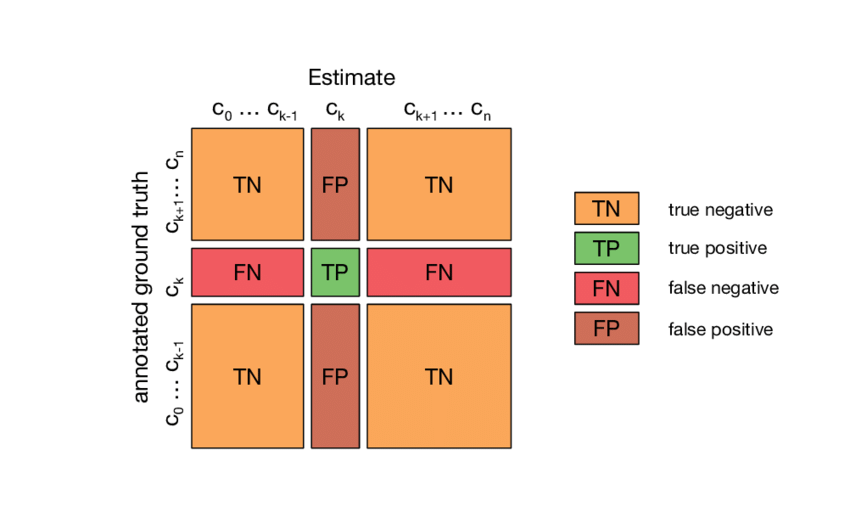
\includegraphics[scale=0.4]{Images/confusion_matrix.png}
    \caption{Confusion matrix for multiclass problem~\cite{ConfusionMatrix}.}
    \label{fig:confusionMatrix}
\end{figure}

\textbf{Accuracy}: Accuracy is the ratio of correctly classified samples to the total number of samples. It is calculated as:
\begin{equation}
    \text{Accuracy} = \frac{\sum_{i=1}^{m} TP_i + \sum_{i \neq j} TN_{ij}}{\sum_{i=1}^{m} (TP_i + FN_i + FP_i + TN_i)}
\end{equation}

\textbf{Precision}: Precision for a class $i$ measures the proportion of correctly predicted instances of class $i$ to the total instances predicted as class $i$. It is given by:
\begin{equation}
    \text{Precision}_i = \frac{TP_i}{TP_i + FP_i}
\end{equation}

\textbf{Recall}: Recall for a class $i$, also known as Sensitivity, measures the proportion of correctly predicted instances of class $i$ to all actual instances of class $i$. The formula is:
\begin{equation}
    \text{Recall}_i = \frac{TP_i}{TP_i + FN_i}
\end{equation}

\textbf{Macro-Averaged Precision and Recall}: To obtain a single performance metric across all classes, macro-averaging can also be used. This approach calculates the precision and recall for each class individually and then averages these values. Macro-averaging treats all classes equally, regardless of their size.

The macro-averaged precision is given by:
\begin{equation}
    \text{Macro Averaged Precision} = \frac{1}{m} \sum_{i=1}^{m} \text{Precision}_i
\end{equation}

The macro-averaged recall is given by:
\begin{equation}
    \text{Macro Averaged Recall} = \frac{1}{m} \sum_{i=1}^{m} \text{Recall}_i
\end{equation}

\textbf{F1 Score}: The F1 score for a class $i$ is the harmonic mean of precision and recall, providing a single metric that balances both concerns. It is calculated as:
\begin{equation}
\text{F1 Score}_i = 2 \times \frac{\text{Precision}_i \times \text{Recall}_i}{\text{Precision}_i + \text{Recall}_i}
\end{equation}
For multiclass problems, the average F1 score across all classes can be used:
\begin{equation}
\text{F1 Score (Macro)} = \frac{1}{m} \sum_{i=1}^{m} \text{F1 Score}_i
\end{equation}

\textbf{Receiver Operating Characteristic (ROC)}: The ROC curve is a graphical plot that illustrates the diagnostic ability of a binary classifier system as its discrimination threshold is varied. The curve is created by plotting the true positive rate (TPR) against the false positive rate (FPR) at various threshold settings. For multiclass classification, ROC curves can be plotted using a one-vs-rest approach, where each class is compared against all other classes.

\begin{figure}[H]
    \centering    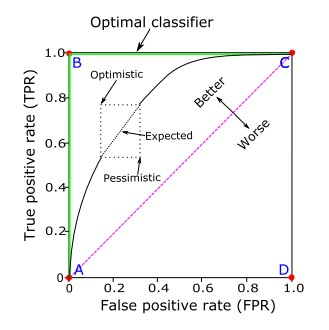
\includegraphics[scale=0.8]{Images/roc_curve.jpg}
    \caption{A basic ROC curve illustrating key points, along with the optimistic, pessimistic, and expected ROC segment~\cite{ClassificationMetrics}.}
    \label{fig:roc_curve}
\end{figure}


\textbf{Area Under the Curve (AUC)}: The AUC is a performance measurement for classification problems at various threshold settings. The AUC represents the degree or measure of separability; it tells how much the model is capable of distinguishing between classes. The AUC is calculated as the area under the Receiver Operating Characteristic (ROC) curve. The ROC curve is a plot of the true positive rate (TPR) against the false positive rate (FPR) at various threshold levels. For a multiclass problem, AUC is computed by considering each class versus the rest.

The AUC is given by:
\begin{equation}
    \text{AUC} = \int_{0}^{1} \text{TPR}(\text{FPR}^{-1}(x)) \, dx
\end{equation}

where:

\begin{equation}
    TPR = \frac{TP}{TP + FN}
\end{equation}

and:

\begin{equation}
    FPR = \frac{FP}{FP + TN}
\end{equation}

For multiclass problems, the AUC can be calculated using a one-vs-rest approach where the ROC curve is plotted for each class against all other classes, and then the average AUC is computed.

\textbf{Macro-Averaged AUC}: Similar to macro-averaging for precision and recall, the macro-averaged AUC is calculated by averaging the AUC values of each class.

The macro-averaged AUC is given by:
\begin{equation}
    \text{Macro Averaged AUC} = \frac{1}{m} \sum_{i=1}^{m} \text{AUC}_i
\end{equation}

\section{Saliency maps}

Saliency maps, used in these experiments, enable the visualization of pixels that had the most significant impact on the decision made by a convolutional neural network. This is achieved by creating a heat map or other graphical representation with dimensions equal to the analyzed image, where pixels with greater influence on the decision have higher values. Saliency maps provide deeper insight into the network's decision-making process, which can lead to the development of better network architectures. Additionally, they allow us to identify incorrectly made decisions by the network. Before the discovery of saliency maps, improving network architectures was limited to trial and error, which was highly unsatisfactory from a scientific point of view.

Two of the most popular methods for generating saliency maps are \textbf{\textit{Grad-CAM}} and \textbf{\textit{Grad-CAM++}}. \textit{Grad-CAM} (Gradient-weighted Class Activation Mapping) uses the gradients of any target concept, flowing into the final convolutional layer to produce a coarse localization map highlighting the important regions in the image for predicting the concept. \textit{Grad-CAM++} is an improved version that provides better localization and sharper visualizations by considering the positive partial derivatives of the gradients with respect to the feature maps. These methods have become widely used due to their effectiveness and ease of interpretation.

The image below demonstrates the application of \textit{Grad-CAM++} to understand the reason for prediction errors made by a convolutional neural network.

\begin{figure}[H]
    \centering    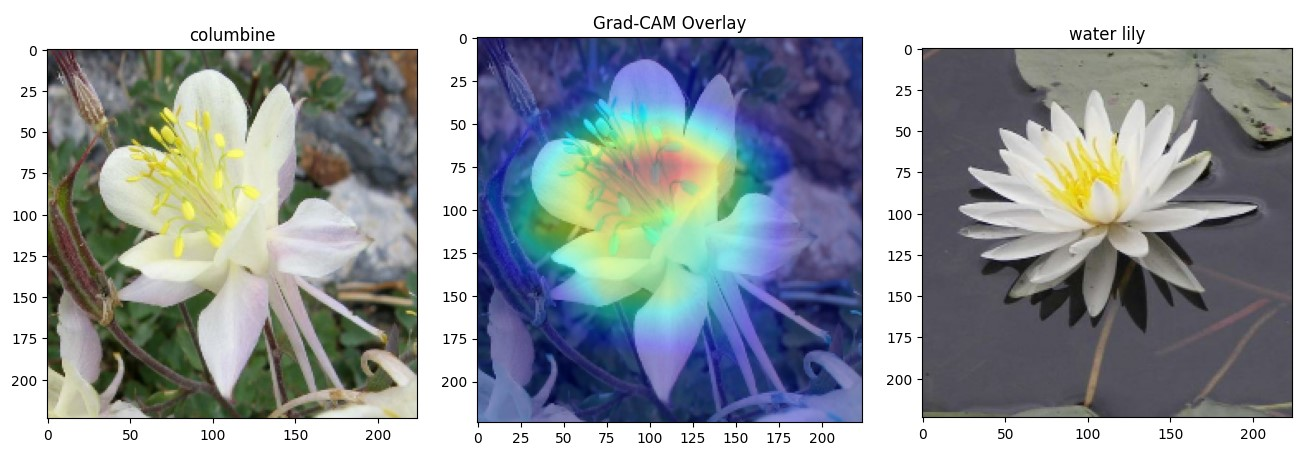
\includegraphics[scale=0.4]{Images/gradcam_mine_example.jpg}
    \caption{\textit{Grad-CAM++} Example.}
    \label{fig:gradcamMine}
\end{figure}

In the left image, we see the original flower (columbine) that was used for prediction. The middle image shows a \textit{Grad-CAM++} visualization overlay, highlighting the regions that the network focused on to make its prediction. The right image shows a sample from the class that the network predicted (water lily).


Using the \textit{Grad-CAM++} visualization, it is evident that the network heavily focused on the yellow part of the flower. Both the columbine and the water lily have prominent yellow sections, likely causing the network to misclassify the columbine as a water lily. Saliency maps, such as the \textit{Grad-CAM++} visualization, help us understand why such mistakes occur. This understanding enables us to refine and improve our model by adjusting the training data, augmenting features, or rethinking the network architecture to reduce similar errors in the future.
    \chapter{Experiments and Results}
\label{cha:ExperimentalSetup}

In this chapter, the results of data augmentation are presented, followed by an interpretation of these results and the implications of the findings. Most of the experiments were repeated several times but only one learning curve and metric value for average results are presented to ensure clarity of visualizations. The primary objective was to observe data augmentation's effects rather than train the best possible model. Consequently, state-of-the-art base models were utilized where many parameters were left trainable, and more epochs were often used than might have been necessary.

\section{Results of Data Augmentation on CNN Performance}
\label{sec:results}

\subsection{Flowers 102}
\label{ssec:resultsFlowers}

First, the performance of the state-of-the-art ResNet50 neural network trained on the Flowers 102 dataset \textbf{without using data augmentation techniques} was analyzed. To evaluate the model's performance, the learning curves for training and validation accuracy, alongside the AUC metric, were plotted and presented in Figure \ref{fig:flowersNoAug}.


\begin{figure}[!htb]
    \centering
    \begin{subfigure}{\textwidth}
        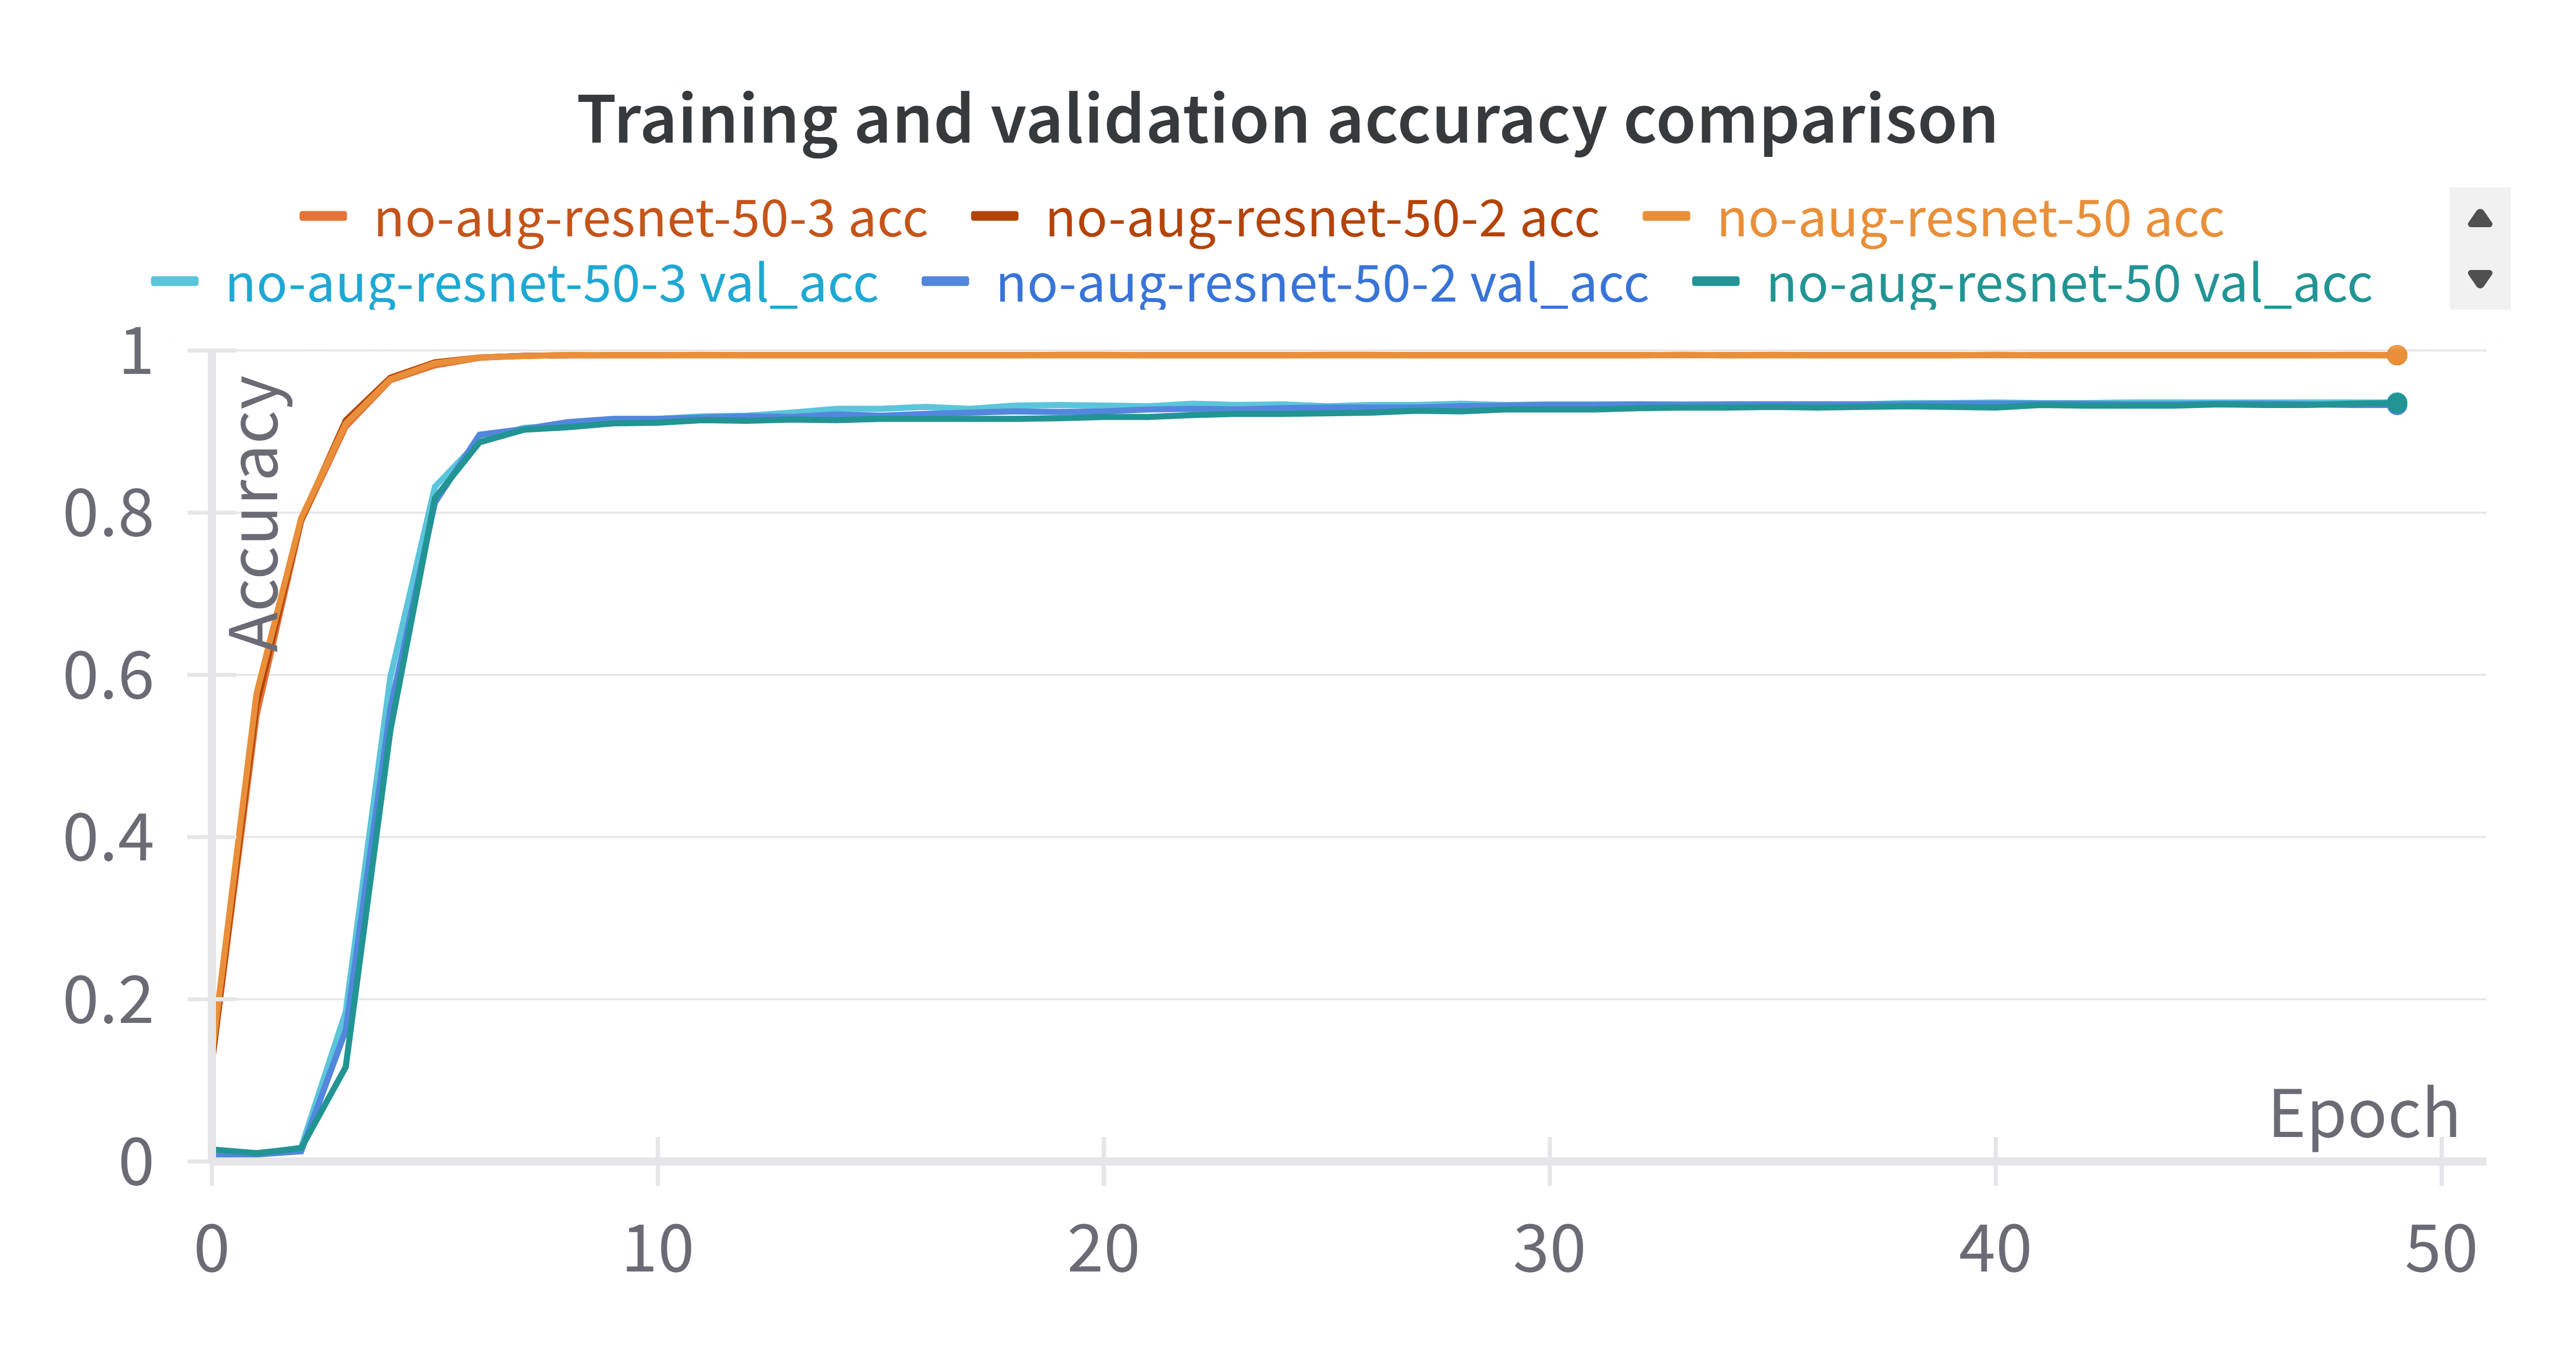
\includegraphics[width=0.95\textwidth]{Images/flowers-results/Flowers-no-aug-acc.png}
        \caption{Training vs Validation Accuracy}
    \end{subfigure}
    \vspace{0.3cm}
    
    \begin{subfigure}{\textwidth}
        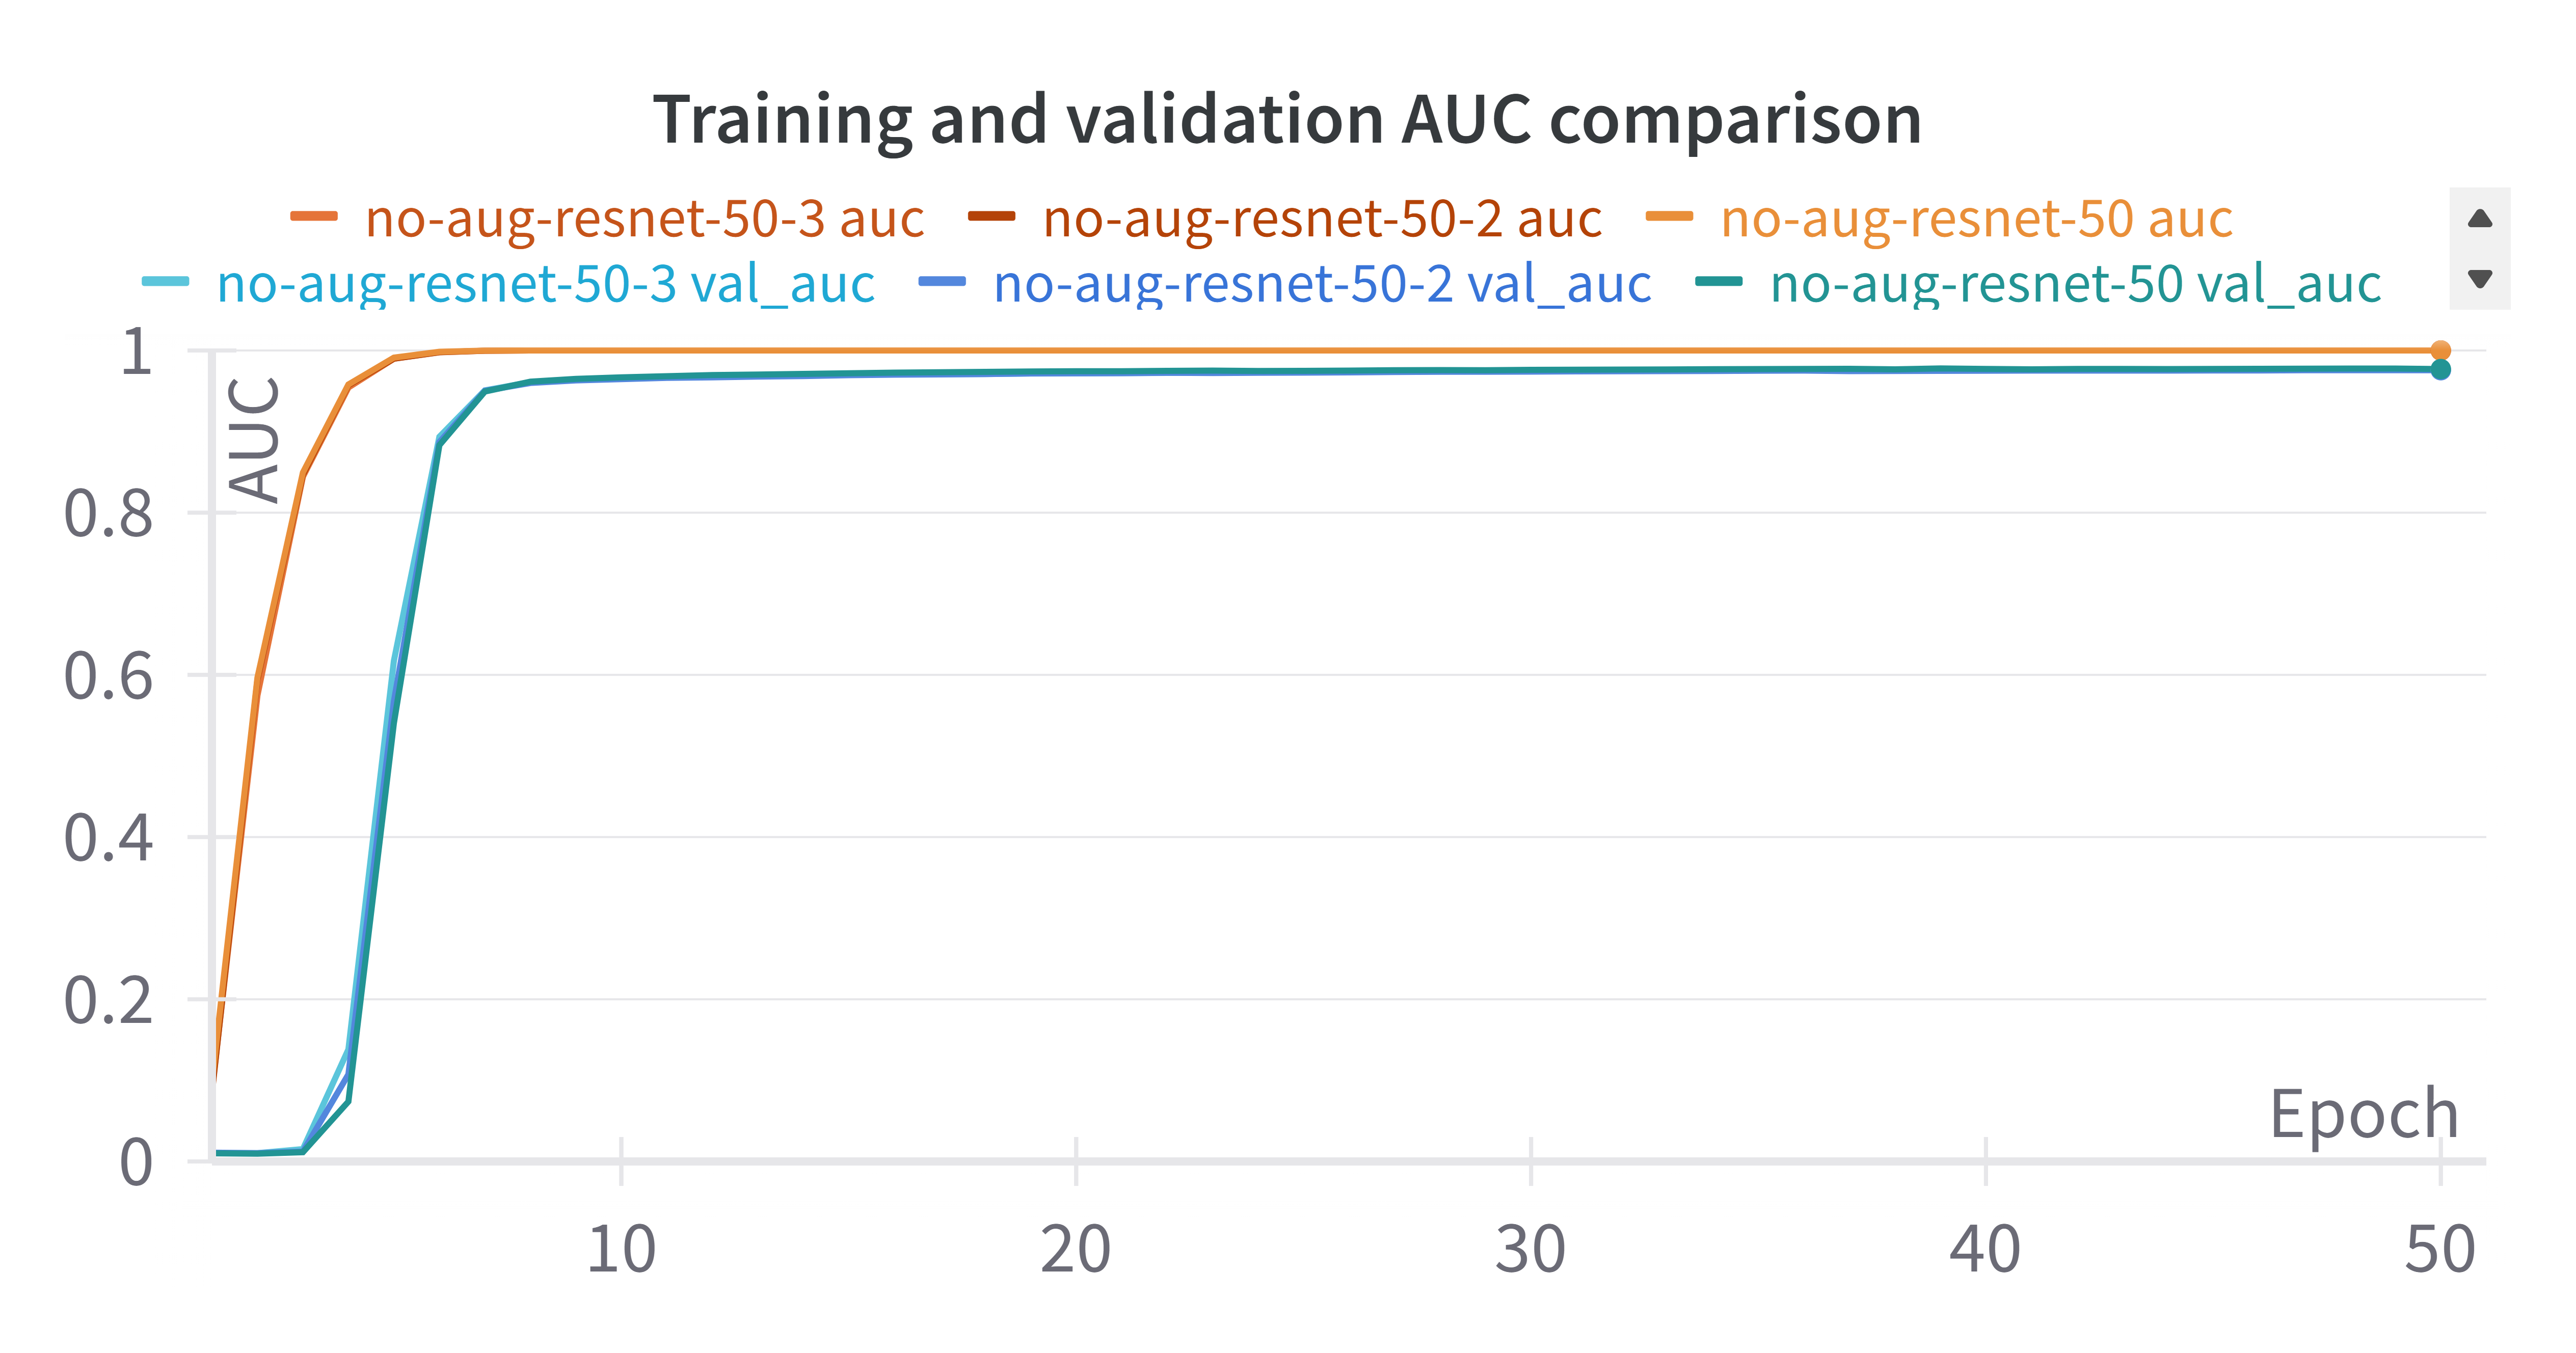
\includegraphics[width=0.95\textwidth]{Images/flowers-results/Flowers-no-aug-auc.png}\
        \caption{Training vs Validation AUC}
    \end{subfigure}
    \vspace{0.3cm}

    \caption{Learning curves for training and validation metrics without data augmentation.}
    \label{fig:flowersNoAug}
\end{figure}

The learning curves indicate that the model improves during the first 10 epochs but does not benefit significantly from further training. This experiment was repeated three times, producing consistent results in each trial.  Moreover, the model suffers overfitting, which becomes even more evident when examining Table \ref{tab:flowersNoAug}. The metrics for the best epoch show that both the training accuracy and AUC approach 1, indicating that the model is mainly memorizing the training data, which does not lead to achieving the highest possible level of generalization.

\begin{table}[h]
    \centering
    \caption{Performance metrics for the best epoch without data augmentation.}
    \begin{tabular}{|c|c|c|c|}
        \hline
        \textbf{Metric} & \textbf{Training} & \textbf{Validation}   \\ \hline
        Accuracy & 99.42 & 93.43 \\ \hline
        AUC & 1 & 0.974  \\ \hline
    \end{tabular}
    \label{tab:flowersNoAug}
\end{table}

Table \ref{tab:testFlowersNoAug} presents the performance metrics calculated on the test set. All values hover around 0.94, which is similar to the validation set metrics. To prevent the model from simply memorizing specific cases and to encourage it to learn more advanced features for effective classification, data augmentation techniques were employed.

\begin{table}[h]
    \centering
    \caption{Test Metrics for the best model without augmentation.}
    \label{tab:testFlowersNoAug}
    \begin{tabular}{|c|c|}
        \hline
        \textbf{Metric} & \textbf{Value} \\
        \hline
        Test Accuracy & 94.12 \\
        Precision & 94.03 \\
        Recall & 94.11 \\
        F1 Score & 93.87 \\
        \hline
    \end{tabular}
\end{table}

First, individual traditional data augmentation techniques were utilized and compared. The methods used at this stage include rotations by angles between -45 and 45 degrees, horizontal flipping, color adjustments (contrast and brightness), random zooming on parts of the input image, and the addition of Gaussian noise and Gaussian filtering. 

All augmentation techniques were carefully constrained to avoid unrealistic alterations of the flowers, such as excessive rotation, vertical flipping, extreme zoom, or overwhelming noise. This ensured that the flowers remained recognizable and reflective of their natural appearance. The results of these experiments are displayed in Table \ref{tab:testFlowersTradCompare}.

\begin{table}[b!]
\centering
\caption{Traditional augmentation comparison.}
\begin{tabular}{| >{\centering\arraybackslash}m{2.5cm} ! {\vrule width 1.5pt} >{\centering\arraybackslash}m{1.0cm} | >{\centering\arraybackslash}m{1.0cm} !{\vrule width 1.5pt} >{\centering\arraybackslash}m{1.0cm} | >{\centering\arraybackslash}m{1.0cm} !{\vrule width 1.5pt} >{\centering\arraybackslash}m{1.0cm} | >{\centering\arraybackslash}m{1.0cm} | >{\centering\arraybackslash}m{1.0cm} | >{\centering\arraybackslash}m{1.0cm} |}
\hline
\multirow{2}{*}{\textbf{Augmentation}} & \multicolumn{2}{c!{\vrule width 1.5pt}}{\textbf{Train}} & \multicolumn{2}{c!{\vrule width 1.5pt}}{\textbf{Val}} & \multicolumn{4}{c|}{\textbf{Test}} \\
\cline{2-9}
 & \textbf{Acc} & \textbf{AUC} & \textbf{Acc} & \textbf{AUC}  & \textbf{Acc} & \textbf{Prec.} & \textbf{Recall} & \textbf{F1} \\
\hline
no-aug & 99.42 & 1 & 93.43 & 0.976 & 94.12 & 94.03 & 94.12 & 93.84 \\
\hline
flip & 99.42 & 1 & 94.84 & 0.982 & 94.99 & 94.83 & 94.99 & 94.75 \\
\hline
\textbf{cropping} & 99.42 & 1 & \textbf{95.23} & \textbf{0.981} & 95.60 & 95.39 & 95.60 & 95.35 \\
\hline
\textbf{rotate45}  & \textbf{99.39} & 1 & 94.92 & 0.981 & \textbf{95.91} & \textbf{95.62} & \textbf{95.91} & \textbf{95.62} \\
\hline
color & 99.42 & 1 & 93.75 & 0.978 & 94.99 & 94.86 & 94.99 & 94.62 \\
\hline
gn-noise & 99.42 & 1 & 93.44 & 0.978 & 94.93 & 94.78 & 94.93 & 94.59 \\
\hline
gn-filter & 99.42 & 1 & 94.14 & 0.978 & 94.93 & 94.80 & 94.93 & 94.65 \\
\hline
\end{tabular}
\label{tab:testFlowersTradCompare}
\end{table}

To begin with, we can see that traditional data augmentation techniques used in this experiment did not impact the training accuracy and AUC values. However, there was a noticeable improvement in the validation and test metrics for every augmentation technique applied. 

For the validation set, most accuracy values, except Gaussian noise augmentation, increased by one percentage point, which is significant, considering the initial validation accuracy was 93.4\%. Notably, cropping had the best results, with the validation accuracy increasing to 95.2\%, a rise of 1.8\%.

Similar improvements were observed in the test set metrics. The baseline accuracy without augmentation was 94.1\%. This value increased with every augmentation technique. Specifically, the accuracy improved by approximately 1.5 and 1.8 percentage points for \textbf{rotation} and \textbf{cropping}, respectively.

As mentioned before, despite the increased validation and test set metrics, the application of these augmentation methods individually did not decrease the training set metrics values, which remained close to 100\%. The next step involved investigating whether combining all augmentation techniques, with varying probabilities of application, could make the training set more challenging. This approach aimed to potentially decrease the model's performance on the training data while further improving validation and test set results.

Figure \ref{fig:flowersLCAugComparison} presents a comparison of the training and validation accuracy learning curves under three conditions: without data augmentation, with all traditional augmentations applied, and with advanced augmentation, which includes all types of augmentations, such as \textit{CutMix} and \textit{MixUp}.

\begin{figure}[!htb]
    \centering
    \begin{subfigure}{0.95\textwidth}
        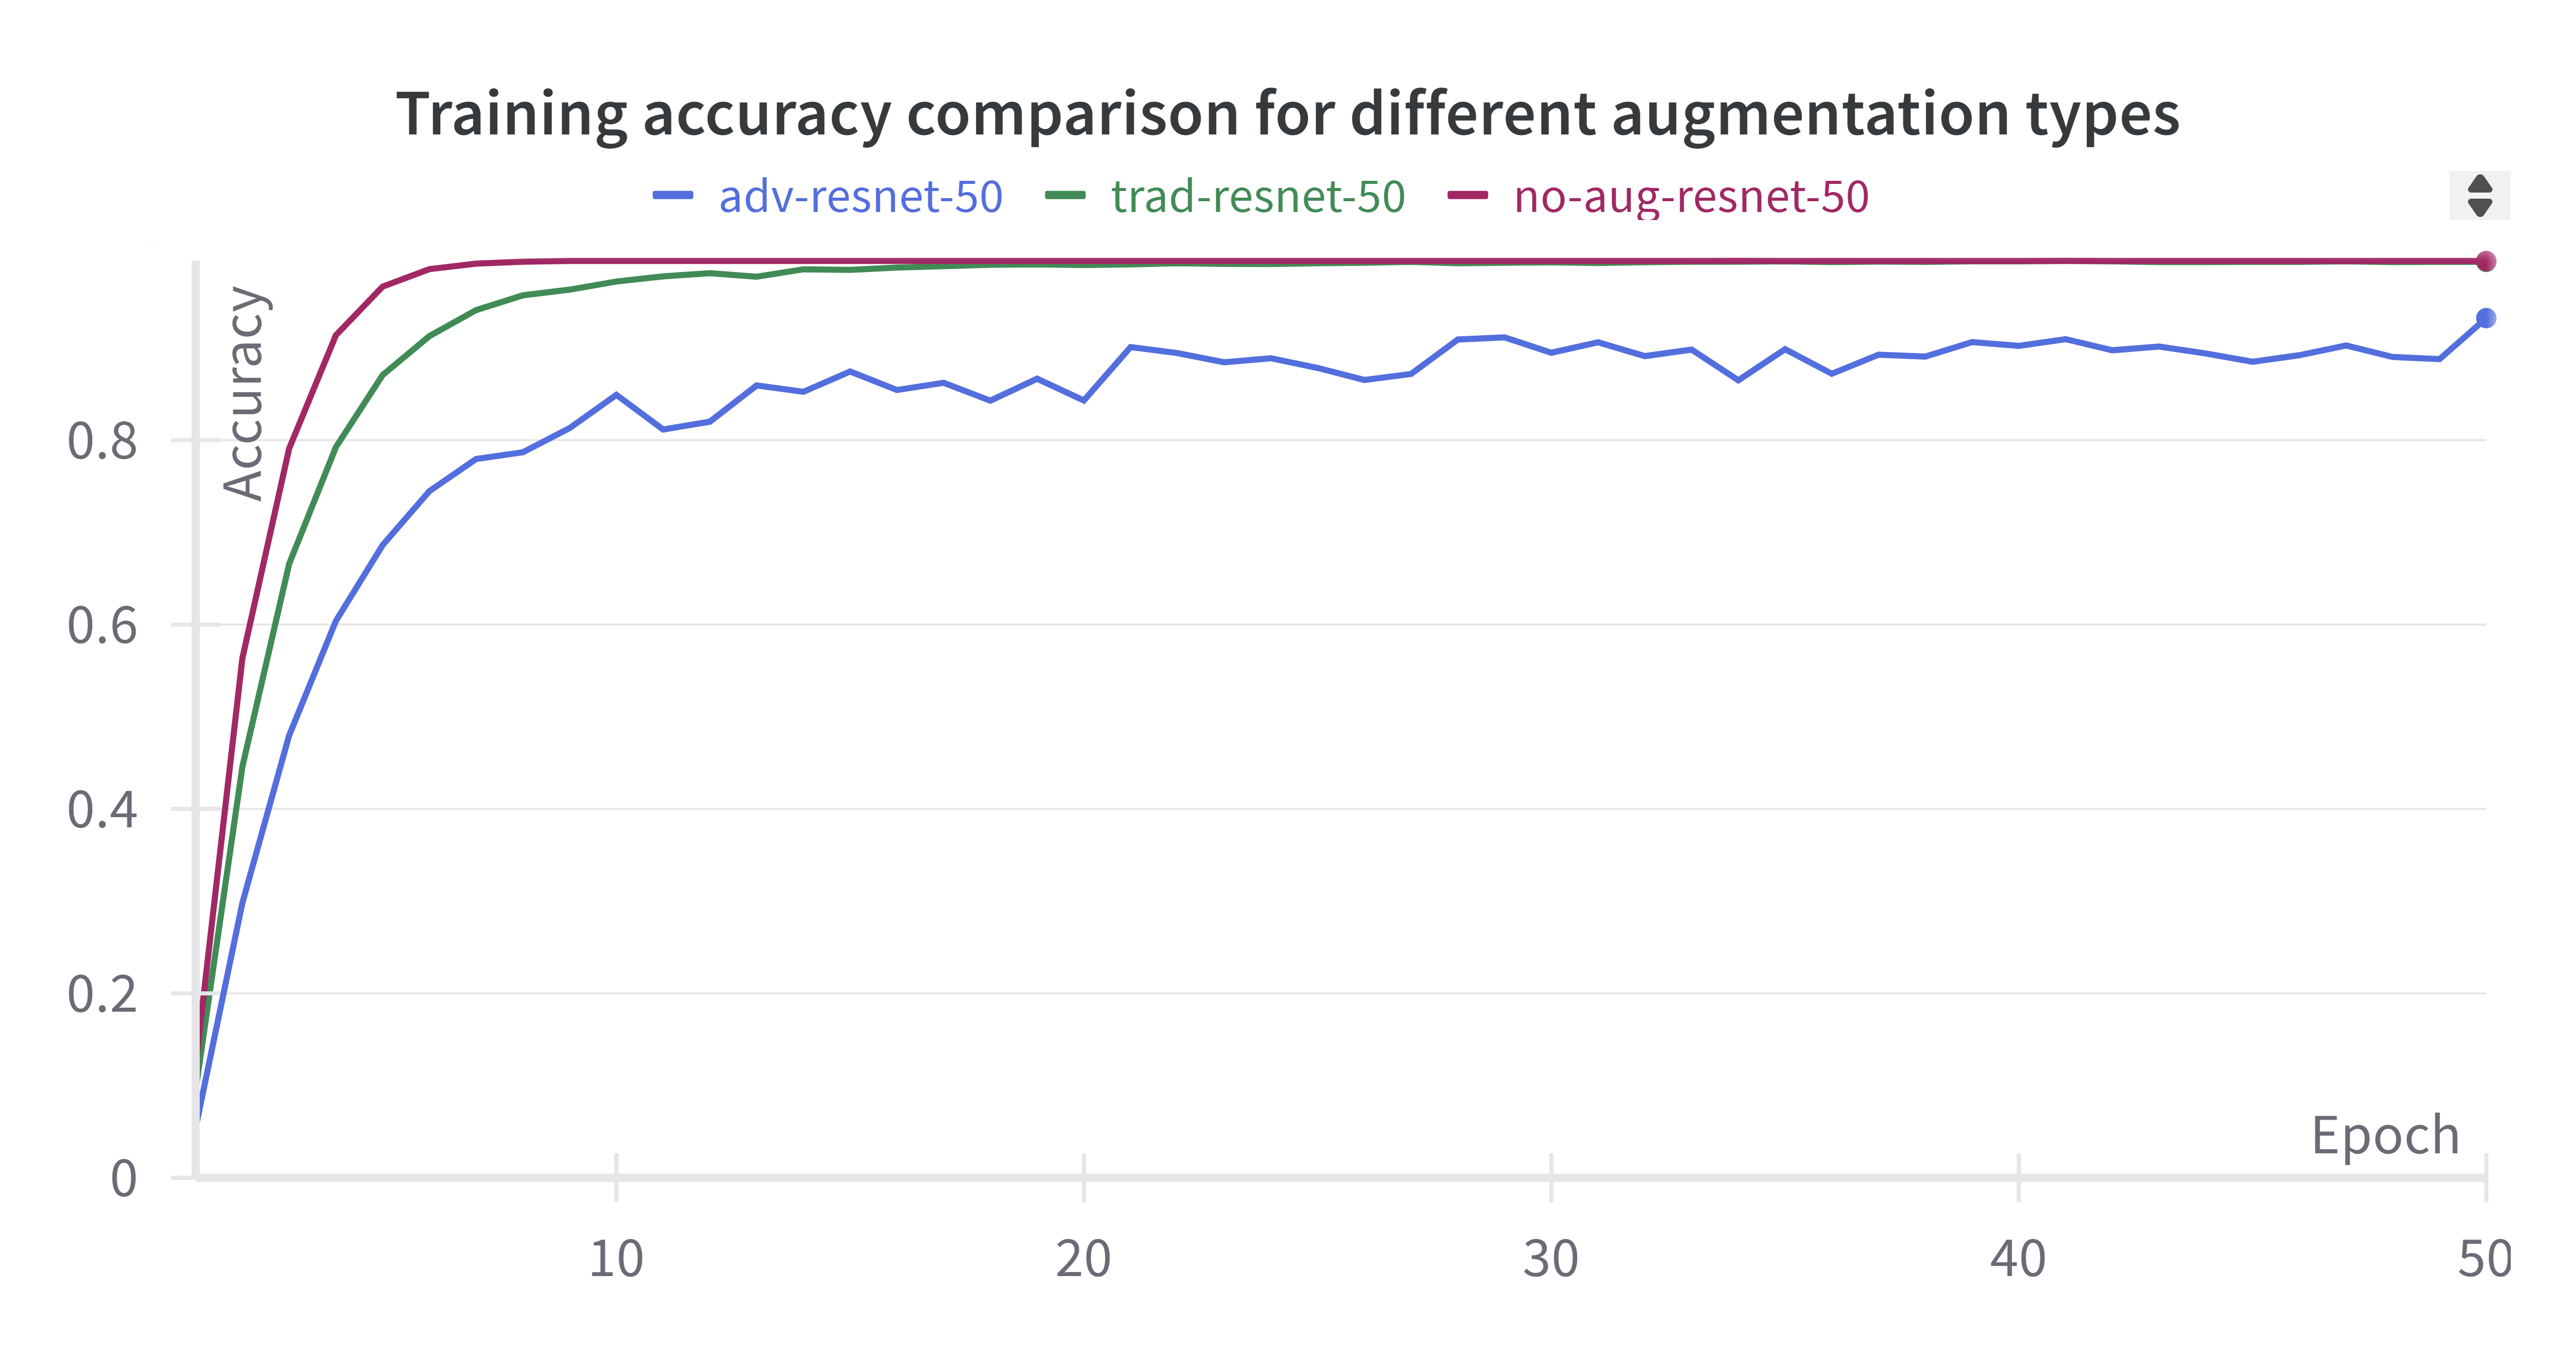
\includegraphics[width=\textwidth]{Images/flowers-results/Learning-Curves-Train-Aug-Comparison.png}
        \caption{Training Accuracy}
    \end{subfigure}
    \vspace{0.3cm}

    \begin{subfigure}{0.95\textwidth}
        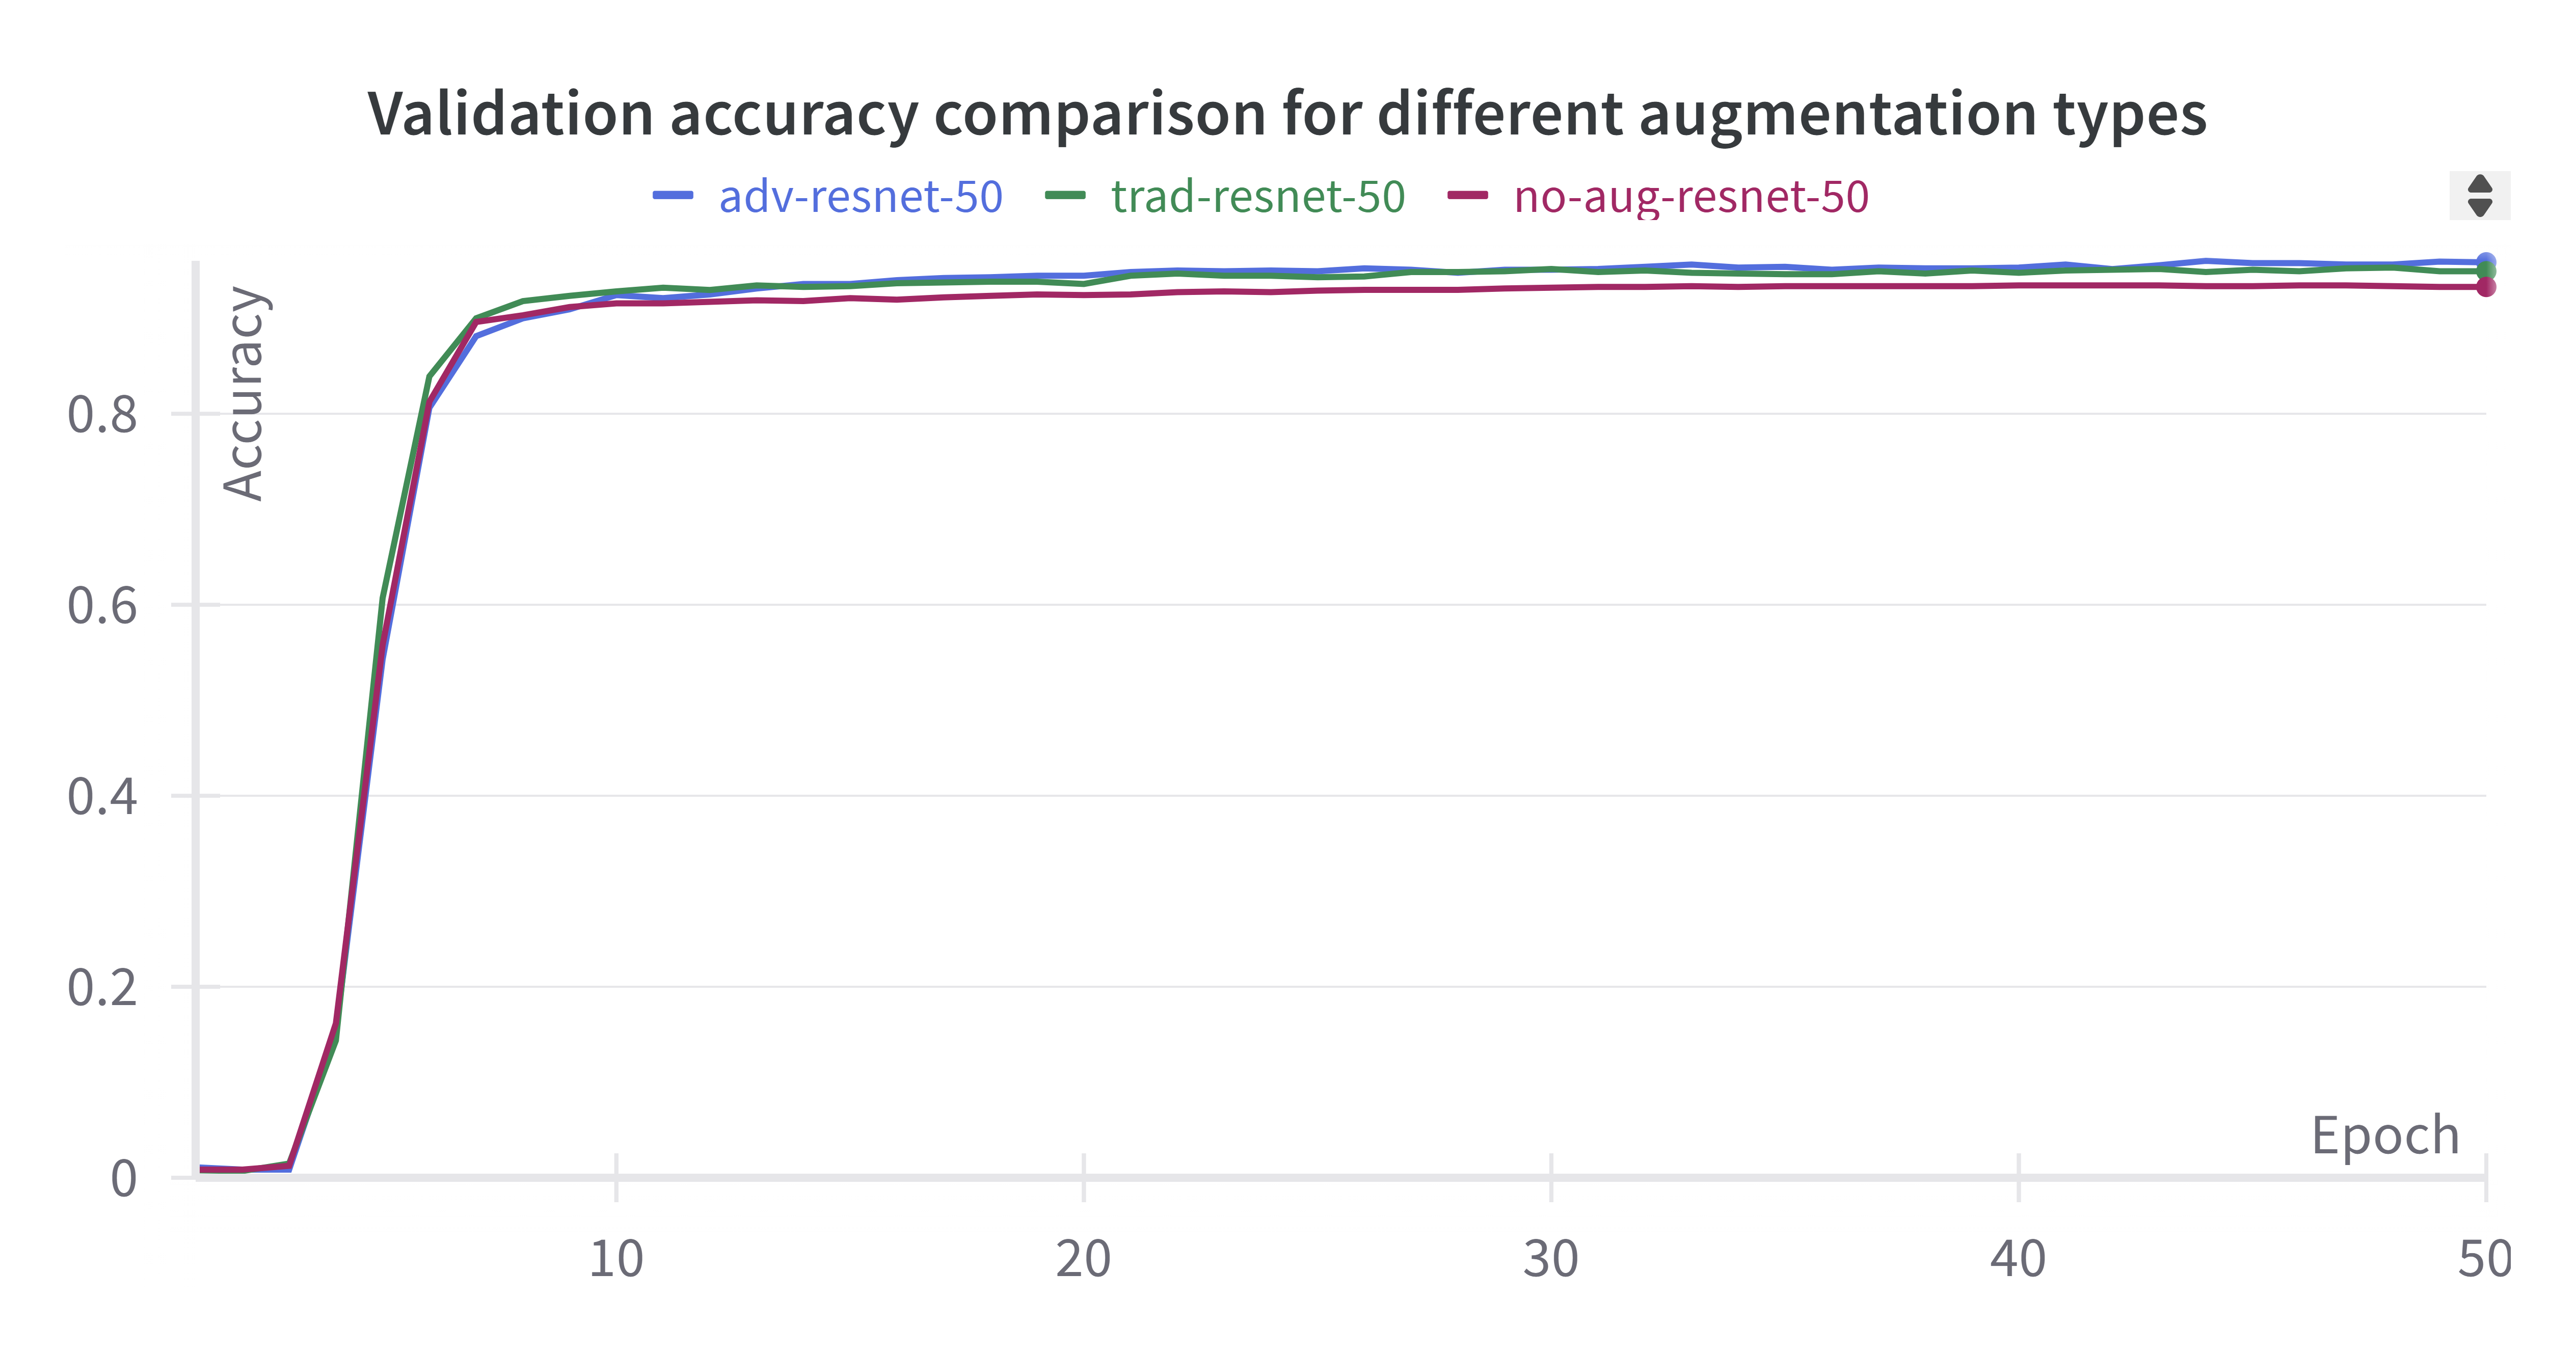
\includegraphics[width=\textwidth]{Images/flowers-results/Learning-Curves-Val-Aug-Comparison.png}\
        \caption{Validation Accuracy}
    \end{subfigure}
    \vspace{0.3cm}
    \caption{Training and validation accuracy learning curves comparison for different augmentation types.}
    \label{fig:flowersLCAugComparison}
\end{figure}

The best validation results are achieved by combining all data augmentation techniques together, referred to as \textbf{adv-resnet-50} on the plot. Although the difference is minimal, traditional augmentation techniques yield slightly lower performance. In contrast, the absence of augmentation techniques results in worse generalization, where the model's performance on the training set does not translate effectively to the validation and test sets.

\begin{figure}[!h]
    \centering
    \begin{subfigure}{0.75\textwidth}
        \centering
        \includegraphics[width=\textwidth]{Images/flowers-results/LC-Train-Val-No-Aug.png}
        \caption{No Augmentation}
    \end{subfigure}
    \vspace{0.3cm}

    \begin{subfigure}{0.75\textwidth}
        \centering
        \includegraphics[width=\textwidth]{Images/flowers-results/LC-Train-Val-Trad-Aug.png}\
        \caption{Traditional Augmentation}
    \end{subfigure}
    \vspace{0.3cm}

    \begin{subfigure}{0.75\textwidth}
        \centering
        \includegraphics[width=\textwidth]{Images/flowers-results/LC-Train-Val-Adv-Aug.png}
        \caption{Advanced Augmentation}
    \end{subfigure}
    \vspace{0.3cm}

    \caption{Learning Curves for each augmentation technique separately.}
    \label{fig:LCSeparately}
\end{figure}

Figure \ref{fig:LCSeparately} shows comparison of learning curves -- training and validation -- separately, for each augmentation technique described above. It is important to note that when data augmentation is used, the training dataset becomes much more challenging, and the point where the values of training metrics are lower than the values of validation and test metrics is achieved. This indicates that the model has \textbf{difficulty accurately classifying training examples}, but through this challenge, \textbf{it learns advanced features that improve its ability to recognize simpler validation and test examples} not encountered during parameter updates. The numerical values of the learning curves described above are shown in Table \ref{tab:FlowersBestEpoch}.

\begin{table}[h!]
\centering
\caption{Accuracy and AUC metrics for the best epoch using combined augmentation techniques.}
\begin{tabular}{| >{\centering\arraybackslash}m{2.5cm} !{\vrule width 1.5pt} >{\centering\arraybackslash}m{1.0cm} | >{\centering\arraybackslash}m{1.0cm} !{\vrule width 1.5pt} >{\centering\arraybackslash}m{1.0cm} | >{\centering\arraybackslash}m{1.0cm} !{\vrule width 1.5pt} }
\hline
\multirow{2}{*}{\textbf{Augmentation}} & \multicolumn{2}{c!{\vrule width 1.5pt}}{\textbf{Train}} & \multicolumn{2}{c!{\vrule width 1.5pt}}{\textbf{Val}} \\
\cline{2-5}
 & \textbf{Acc} & \textbf{AUC} & \textbf{Acc} & \textbf{AUC} \\
\hline
no-aug & 99.42 & 0.999 & 93.44 & 0.975 \\
\hline
trad-aug & 99.31 & 0.999 & 95.31 & 0.983 \\
\hline
adv-aug & 89.40 & 0.600 & 96.02 & 0.986 \\
\hline
\end{tabular}
\label{tab:FlowersBestEpoch}
\end{table}

Looking at the table above, we should pay attention to the training accuracy and AUC values for advanced augmentation. Although the training accuracy is 10 percentage points lower than that of other individual and combined augmentation methods, this does not imply poor performance on the validation and test sets. On the contrary, this network performs the best among all analyzed above.

Secondly, we can draw conclusions about the AUC metric. While traditional augmentation does not affect its value, advanced augmentation, which includes \textit{MixUp} and \textit{CutMix}, significantly lowers the training AUC while maintaining the highest validation AUC among the three methods. These techniques effectively implement a form of label smoothing by blending labels, which reduces the sharp boundaries between classes, making it more challenging for the model to maintain high separability. This leads to lower AUC values during training because the model is being trained on more ambiguous examples.  Consequently, the model learns more robust features, resulting in a high validation AUC.


Figure \ref{fig:testAllAug} shows a comparison of test metrics for models trained using various data augmentation techniques. It displays bar plots of the results from the best epoch for each technique. These results are consistent with the observations on the validation dataset. However, both augmentation methods show more noticeable improvements on the test set, with an increase of around 2 percentage points.

\begin{figure}[!htb]
    \centering
    \begin{subfigure}{0.45\textwidth}
        \includegraphics[width=\textwidth]{Images/flowers-results/test_acc.png}
        \caption{Accuracy}
    \end{subfigure}
    \vspace{0.3cm}
    \hfill
    \begin{subfigure}{0.45\textwidth}
        \includegraphics[width=\textwidth]{Images/flowers-results/test_f1.png}\
        \caption{F1 Score}
    \end{subfigure}
    \vspace{0.3cm}

    \caption{Test metrics for different types of data augmentation.}
    \label{fig:testAllAug}
\end{figure}

\newpage
Data augmentation was also checked for the \textit{EfficientNetB0} model. Even though this model has approximately 5 times fewer parameters than \textit{ResNet50}, it performs slightly better on the \textit{ImageNet} dataset, as illustrated in Figure \ref{fig:efficientNet}. A comparison of learning curves for \textit{EfficientNet} is presented in Figure \ref{fig:efficientLC}.

\begin{figure}[!htb]
    \centering
    \includegraphics[width=0.95\textwidth]{Images/flowers-results/efficientNetLC.png}
    \caption{\textit{EfficientNet} learning curves.}
    \label{fig:efficientLC}
\end{figure}


The plot illustrates the training (dashed line) and validation (solid line) accuracy of models utilizing different data augmentation techniques over $50$ epochs. The yellow lines represent the model without data augmentation, the blue lines correspond to the model with traditional data augmentation, and the green lines depict the model with advanced data augmentation.

The model without data augmentation achieves the highest training accuracy, consistently increasing and achieving almost 100\% by the end of the $50$ epochs. The model with advanced data augmentation has the lowest training accuracy among the three. This might suggest that the advanced augmentation makes the training process more challenging, potentially leading to a more robust and generalized model.

Interestingly, despite the differences in training accuracy, the end validation accuracy for all three models is almost the same. This suggests that, regardless of the augmentation technique used, the models converge to a comparable level of performance on the validation set. \textit{EfficientNet's} performance is better than \textit{ResNet's} performance without data augmentation, but worse than \textit{ResNet's} performance with data augmentation applied. Table \ref{tab:effTable} shows a comparison of the \textit{EfficientNet} metrics for the best epoch. The model trained on the dataset augmented using advanced techniques performed slightly worse on the validation set than the model trained without data augmentation but handles the test set as good as the best model trained on the traditionally augmented dataset. 

\begin{table}[h!]
\centering
\caption{EfficientNet metrics comparison.}
\begin{tabular}{| >{\centering\arraybackslash}m{2.5cm} !{\vrule width 1.5pt} >{\centering\arraybackslash}m{1.0cm} | >{\centering\arraybackslash}m{1.0cm} !{\vrule width 1.5pt} >{\centering\arraybackslash}m{1.0cm} | >{\centering\arraybackslash}m{1.0cm} !{\vrule width 1.5pt} >{\centering\arraybackslash}m{1.0cm} | >{\centering\arraybackslash}m{1.0cm} !{\vrule width 1.5pt} >{\centering\arraybackslash}m{1.0cm}|}
\hline
\multirow{2}{*}{\textbf{Augmentation}} & \multicolumn{2}{c!{\vrule width 1.5pt}}{\textbf{Train}} & \multicolumn{2}{c!{\vrule width 1.5pt}}{\textbf{Val}} & \multicolumn{2}{c!{\vrule width 1.5pt}}{\textbf{Test}} \\
\cline{2-7}
 & \textbf{Acc} & \textbf{AUC} & \textbf{Acc} & \textbf{AUC} & \textbf{Acc} & \textbf{F1} \\
\hline
no-aug & 99.25 & 99.99 & 94.38 & 98.12 & 94.08 & 93.80 \\
\hline
trad-aug & 97.55 & 99.65 & 94.77 & 98.47 & 94.81 & 94.53 \\
\hline
adv-aug & 85.81 & 56.66 & 94.14 & 98.25 & 94.81 & 94.49 \\
\hline
\end{tabular}
\label{tab:effTable}
\end{table}

The plot in Figure \ref{fig:effResLC} compares the training accuracy of \textit{EfficientNet} and \textit{ResNet} models \textbf{without data augmentation} over $35$ epochs. The yellow line represents the training accuracy of the \textit{EfficientNet} model, while the purple line represents the training accuracy of the \textit{ResNet} model. 

\begin{figure}[!h]
    \centering
    \includegraphics[width=0.95\textwidth]{Images/flowers-results/efficient-resnet-no-aug-lc.png}
    \caption{EfficientNet and ResNet learning curves without data augmentation.}
    \label{fig:effResLC}
\end{figure}

The \textit{ResNet} model converges much faster than the \textit{EfficientNet} model, achieving 98\% of the training accuracy after only $5$ epochs and stabilizing earlier. It means that the \textit{ResNet} model overfits the training data having more parameters than the \textit{EfficientNet} model while \textit{EfficientNet} keeps learning throughout all the epochs. This observation aligns with previous experiments showing that \textit{EfficientNet-B0}, with its $4$ million parameters, does not benefit from data augmentation as much as \textit{ResNet}, which has $20$ million parameters. The larger capacity of \textit{ResNet} allows it to leverage augmented data more effectively, improving its performance significantly. \textit{EfficientNet}, being a more parameter-efficient model, shows less pronounced benefits from data augmentation, suggesting it relies more on its architectural efficiency and less on extensive data augmentation for high accuracy.

\begin{figure}[!h]
    \centering
    \begin{subfigure}[b]{0.65\textwidth}
        \centering
        \includegraphics[width=\textwidth]{Images/flowers-results/confusion_matrix_no_aug.png}
        \caption{Without augmentation}
    \end{subfigure}

    \begin{subfigure}[b]{0.65\textwidth}
        \centering
        \includegraphics[width=\textwidth]{Images/flowers-results/confusion_matrix_adv_aug.png}
        \caption{With advanced augmentation}
    \end{subfigure}
    \caption{Confusion matrices for the top 10 worst-performing species of flowers.}
    \label{fig:confMatricesFlowersEfficient}
\end{figure}

Because Flowers dataset contains $102$ classes, plotting the complete confusion matrix is not practical. Figure \ref{fig:confMatricesFlowersEfficient} shows \textbf{confusion matrices} for the top $10$ worst-performing flower species before and after data augmentation. These species were selected based on the proportion of misclassified samples. 


The confusion matrices reveal that while data augmentation slightly improves the results for most of these worst-performing species, it does not affect the classification of the \textit{blackberry lily}, which remains entirely misclassified in both models.

For the final comparison, saliency maps were used to examine what the model focuses on with and without augmentation. These evaluations were done manually, and the implications of the findings are summarized below.

In most cases, both networks focus on similar areas of the input image, as shown in Figure \ref{fig:saliency1}. This is expected since the accuracy of the models is not much different.

\begin{figure}[h!]
    \centering
    \begin{subfigure}[b]{0.32\textwidth}
        \centering
        \includegraphics[width=\textwidth]{Images/saliency-flowers/510/image_510.png}
        \caption{Preprocessed image}
    \end{subfigure}
    \hfill
    \begin{subfigure}[b]{0.32\textwidth}
        \centering
        \includegraphics[width=\textwidth]{Images/saliency-flowers/510/GradCAM_510_no_aug.png}
        \caption{Without augmentation}
    \end{subfigure}
    \hfill
    \begin{subfigure}[b]{0.32\textwidth}
        \centering
        \includegraphics[width=\textwidth]{Images/saliency-flowers/510/GradCAM_510_aug.png}
        \caption{With augmentation}
    \end{subfigure}
    \caption{Similar saliency maps with and without augmentation.}
    \label{fig:saliency1}
\end{figure}

The biggest difference appears when a model trained without data augmentation makes mistakes that a model trained with augmented data avoids. Figure \ref{fig:saliency2} shows this with a \textit{lotus} flower example. The saliency map for the first model, trained without augmentation highlights the yellow stamen of the flower, causing confusion with the \textit{columbine} flower, which also has prominent yellow parts. In contrast, the model trained on augmented data focused on the leaves and correctly classified the example.

\begin{figure}[h!]
    \centering
    \begin{subfigure}[b]{0.24\textwidth}
        \centering
        \includegraphics[width=\textwidth]{Images/saliency-flowers/172/image_172.png}
        \caption{Input image}
    \end{subfigure}
    \hfill
    \begin{subfigure}[b]{0.24\textwidth}
        \centering
        \includegraphics[width=\textwidth]{Images/saliency-flowers/172/GradCAM_no_aug.png}
        \caption{Without augmentation}
    \end{subfigure}
    \hfill
    \begin{subfigure}[b]{0.24\textwidth}
        \centering
        \includegraphics[width=\textwidth]{Images/saliency-flowers/172/GradCAM_172_aug.png}
        \caption{With augmentation}
    \end{subfigure}
    \hfill
    \begin{subfigure}[b]{0.24\textwidth}
        \centering
        \includegraphics[width=\textwidth]{Images/saliency-flowers/172/image_320_wrong.png}
        \caption{Wrong prediction}
    \end{subfigure}
    \caption{Saliency maps for example misclassified by model trained without data augmentation.}
    \label{fig:saliency2}
\end{figure}

Using saliency maps, we can also visualize samples where data augmentation did not improve the prediction. As mentioned above, the confusion matrix revealed that \textit{blackberry lily} flowers are never correctly classified by any model. Analyzing images presented in Figure \ref{fig:saliency3} we can understand, that the model focused on the background instead of the flower. Augmentation methods which change the background of the image could improve the results.

\begin{figure}[h!]
    \centering
    \begin{subfigure}[b]{0.32\textwidth}
        \centering
        \includegraphics[width=\textwidth]{Images/saliency-flowers/249/image_249.png}
        \caption{Preprocessed image}
    \end{subfigure}
    \hfill
    \begin{subfigure}[b]{0.32\textwidth}
        \centering
        \includegraphics[width=\textwidth]{Images/saliency-flowers/249/GradCAM_249_no_aug.png}
        \caption{Without augmentation}
    \end{subfigure}
    \hfill
    \begin{subfigure}[b]{0.32\textwidth}
        \centering
        \includegraphics[width=\textwidth]{Images/saliency-flowers/249/GradCAM_249_aug.png}
        \caption{With augmentation}
    \end{subfigure}
    \caption{Saliency maps for class which performance did not improve thanks to data augmentation.}
    \label{fig:saliency3}
\end{figure}

The final experiment on this dataset involved over-augmenting the data. The batch of over-augmented data, with a 100\% probability of augmentation application, increased color contrast, and full rotations, is shown in Figure \ref{fig:overaug}. 

\begin{figure}[!h]
    \centering
    \includegraphics[width=0.9\textwidth]{Images/flowers-overaugmented/batch_overaugmented.png}
    \caption{Over-augmented batch.}
    \label{fig:overaug}
\end{figure}

Even though this batch does not appear over-augmented, the unnatural rotations and excessively high probability of application led to worse performance of the model trained on this augmented dataset compared to the unchanged dataset. These results are visible in Figure \ref{fig:overaugLC}. The validation accuracy of the model trained on the over-augmented dataset is around 83\%, which is \textbf{10 percentage points} less than the model trained without data augmentation. These results demonstrate that data augmentation does not always help and should be applied carefully.

\begin{figure}[!h]
    \centering
    \includegraphics[width=0.95\textwidth]{Images/flowers-overaugmented/overaugLC.png}
    \caption{Comparison of learning curves for not augmented and over-augmented dataset.}
    \label{fig:overaugLC}
\end{figure}


\subsection{One-shot Flowers 102}
\label{ssec:resultsOneshotFlowers}

In this experiment, the number of flower samples was limited to $5$, $10$, and $20$ per class to evaluate the effectiveness of data augmentation under \textbf{limited data conditions}. If the number of examples in the original dataset was smaller than the threshold, examples were randomly repeated. This resulted in datasets of $510$, $1020$, and $2040$ samples, respectively, with 80\% used for training and 20\% for validation. Models were trained using $80$, $100$, and $120$ epochs to make stabilization of the training possible. The test set remained the same as in previous experiments ($1638$ examples).

Figures \ref{fig:oneshotLCsTrain} and \ref{fig:oneshotLCsVal} present training and validation learning curves of models trained on all the previously mentioned datasets. Each plot uses consistent colors: yellow represents the model trained on the dataset without data augmentation, orange indicates the use of \textit{MixUp} and \textit{CutMix} methods, blue is associated with traditional techniques, and green is utilized for advanced techniques that combine all the methods mentioned above.

\begin{figure}[!h]
    \centering
    \begin{subfigure}[b]{0.77\textwidth}
        \centering
        \includegraphics[width=\textwidth]{Images/oneshot/lc/train_acc_5.png}
        \caption{Training accuracy - 5 samples}
    \end{subfigure}

    \begin{subfigure}[b]{0.77\textwidth}
        \centering
        \includegraphics[width=\textwidth]{Images/oneshot/lc/train_acc_10.png}
        \caption{Training accuracy - 10 samples}
    \end{subfigure}


    \begin{subfigure}[b]{0.77\textwidth}
        \centering
        \includegraphics[width=\textwidth]{Images/oneshot/lc/train_acc_20.png}
        \caption{Training accuracy - 20 samples}
    \end{subfigure}

    \caption{Training learning curves for different sizes of Flowers 102 dataset.}
    \label{fig:oneshotLCsTrain}
   
\end{figure}

\begin{figure}[!h]
    \centering

    \begin{subfigure}[b]{0.77\textwidth}
        \centering
        \includegraphics[width=\textwidth]{Images/oneshot/lc/val_acc_5.png}
        \caption{Validation accuracy - 5 samples}
    \end{subfigure}


    \begin{subfigure}[b]{0.77\textwidth}
        \centering
        \includegraphics[width=\textwidth]{Images/oneshot/lc/val_acc_10.png}
        \caption{Validation accuracy - 10 samples}
    \end{subfigure}

    \begin{subfigure}[b]{0.77\textwidth}
        \centering
        \includegraphics[width=\textwidth]{Images/oneshot/lc/val_acc_20.png}
        \caption{Validation accuracy - 20 samples}
    \end{subfigure}
    \caption{Validation learning curves for different sizes of Flowers 102 dataset.}
    \label{fig:oneshotLCsVal}
   
\end{figure}

For every dataset size, we observe that the training accuracy reaches 100\% when no augmentation or only traditional augmentation is used. However, with \textit{CutMix} and \textit{MixUp} data augmentation, training accuracy oscillates around 90\%. This is because \textit{MixUp} and \textit{CutMix} make the boundary between examples thinner, as the one-hot encoding is no longer a vector of only zeros and ones. Additionally, these techniques mix images among batches, and in \textit{CutMix}, important parts of the flower can be hidden, making the example difficult to classify correctly. All these factors together make the training process less stable, preventing 100\% accuracy from being reached.


More interesting conclusions can be obtained by looking at the validation accuracy learning curves. First of all, these experiments were repeated several times and the results were similar each time -- applying any kind of augmentation improves the performance of the network. Secondly, the smaller the dataset is, the more it benefits from applying augmentation.

For each dataset size, the influence of \textit{CutMix} and \textit{MixUp} augmentation is the lowest but for the smallest dataset improvement is quite impressive, and very close to other types of augmentations. Advanced augmentation, which combines all methods, yields the best results on the validation set but the difference between traditional augmentation and advanced augmentation is not very large. 

To enable better comparison between different datasets, Figure \ref{fig:oneshotLCSummary} was created. It displays all validation learning curves in a single plot. The colors are consistent: shades of yellow represent the dataset without augmentation, orange for \textit{CutMix} and \textit{MixUp}, blue for traditional augmentation, and green for advanced augmentation. Additionally, darker shades indicate larger dataset sizes. We can observe that larger datasets require fewer epochs to reach a saturation point in accuracy, where the model no longer shows improvement.

\begin{figure}[!h]
    \centering
    \includegraphics[width=\textwidth]{Images/oneshot/lc/summary_val_acc_improved2.png}
    \caption{Comparison of validation learning curves for all datasets and augmentation methods.}
    \label{fig:oneshotLCSummary}
\end{figure}

Moreover, no type of data augmentation can boost model performance as much as doubling the number of training examples. However, the model trained on a dataset with $10$ samples per class using advanced data augmentation performs almost as well as the model trained on a dataset with $20$ samples without any augmentation.

Table \ref{tab:augSampleComparison} presents results for the best epoch of each training as numerical values. Due to the small size of the validation set in limited data conditions, more general conclusions can be drawn by examining the test metrics.

\begin{table}[h!]
\centering
\caption{Augmentation comparison with different sample sizes.}
\begin{tabular}{| >{\centering\arraybackslash}m{1.5cm} | >{\centering\arraybackslash}m{2.2cm} !{\vrule width 1.5pt} >{\centering\arraybackslash}m{1.0cm} | >{\centering\arraybackslash}m{1.0cm} !{\vrule width 1.5pt} >{\centering\arraybackslash}m{1.0cm} | >{\centering\arraybackslash}m{1.0cm} !{\vrule width 1.5pt} >{\centering\arraybackslash}m{1.0cm} | >{\centering\arraybackslash}m{1.0cm} | >{\centering\arraybackslash}m{1.0cm} |}
\hline
\textbf{Samples} & \textbf{Augmentation} & \multicolumn{2}{c!{\vrule width 1.5pt}}{\textbf{Train}} & \multicolumn{2}{c!{\vrule width 1.5pt}}{\textbf{Val}} & \multicolumn{2}{c|}{\textbf{Test}} \\
\cline{3-8}
 &  & \textbf{Acc} & \textbf{AUC} & \textbf{Acc} & \textbf{AUC} & \textbf{Acc} & \textbf{F1} \\
\hline
\multirow{4}{*}{\makecell{5}} & \makecell{no-aug} & 99.22 & 1 & 42.71 & 0.376 & 42.74 & 40.59 \\
 & \makecell{traditional} & 98.96 & 1 & 53.13 & 0.579 & 64.47 & 63.43 \\
 & \makecell{cutmix-mixup} & 94.27 & 0.766 & 54.17 & 0.521 & 56.9 & 54.61 \\
 & \makecell{advanced} & 94.79 & 0.592 & 57.29 & 0.627 & 65.93 & 64.56 \\
\hline
\multirow{4}{*}{\makecell{10}} & \makecell{no-aug} & 99 & 1 & 72.4 & 0.743 & 66.79 & 65.75 \\
 & \makecell{traditional} & 98.87 & 1 & 81.77 & 0.885 & 80.65 & 80.2 \\
 & \makecell{cutmix-mixup} & 94 & 0.6544 & 77.08 & 0.851 & 73.93 & 72.93 \\
 & \makecell{advanced} & 87.25 & 0.615 & 84.38 & 0.910 & 80.34 & 79.73 \\
\hline
\multirow{4}{*}{\makecell{20}} & \makecell{no-aug} & 98.94 & 1 & 86.06 & 91.54 & 81.62 & 81.17 \\
 & \makecell{traditional} & 98.94 & 1 & 92.07 & 0.966 & 88.83 & 88.57 \\
 & \makecell{cutmix-mixup} & 92.19 & 0.648 & 90.14 & 95.04 & 86.87 & 86.34 \\
 & \makecell{advanced} & 91.62 & 0.579 & 93.03 & 0.968 & 88.22 & 87.82 \\
\hline
\end{tabular}
\label{tab:augSampleComparison}
\end{table}

Examining the results of the models trained on the dataset with $5$ samples for each species of flower, we see that the greatest improvement comes from using advanced augmentation techniques. Test accuracy increases from 42.74\% to 65.93\% — a significant improvement of over 23 percentage points for accuracy and 24 percentage points for F1 score. Traditional augmentation gives almost the same improvement, only 1 percentage point less for both metrics. 

For a dataset with $10$ samples per class, the improvement is also notable. All the metrics show enhancement, and while advanced augmentation shows slightly better validation metrics compared to traditional augmentation, the test metrics reveal that traditional augmentation performs slightly better than advanced augmentation.

Even though the validation metrics with augmentation applied on the dataset with $20$ samples per class were almost as good as the ones obtained for the full dataset presented in the previous section, test metrics turned out to be slightly worse. Nonetheless, with this dataset size, data augmentation techniques enable achieving almost 90\% accuracy on the test set with $102$ classes.

Test metrics presented in Table \ref{tab:augSampleComparison} also confirm that data augmentation applied to the dataset can make the model perform almost as well as the one trained on two times bigger dataset. When we apply advanced augmentation to the dataset with $5$ samples per category, we obtain $65.93\%$ test accuracy which is only $0.86$ percentage points less than the one trained on the dataset with 10 samples per category. Similarly, on the dataset with $10$ samples we can achieve $80.65\%$ accuracy, which is $0.97$ percentage points less than for a two times larger dataset.

Figure \ref{fig:testMetricsOneshot} presents test set metrics in the form of bar plots and enable visual comparison of results. The name of each bar indicates the augmentation type and number of samples in each class.

\begin{figure}[!h]
    \centering
    \includegraphics[width=0.95\textwidth]{Images/oneshot/oneshot_test_bar_plot.png}
    \caption{Comparison of test metric values for different augmentation methods and class sizes.}
    \label{fig:testMetricsOneshot}
\end{figure}

Confusion matrices for the top $10$ worst-performing classes in the dataset with $5$ samples per category were plotted in Figure \ref{fig:confMatricesOneshot}. On the left side, we can see that none of these classes are correctly classified. However, when advanced data augmentation methods are applied, the model learns features that enable it to correctly classify some examples, improving overall performance. Similar to the confusion matrix for the full dataset, the confusion matrix still shows no improvement for \textit{blackberry lily}, despite the dataset being balanced. It means that data augmentation applied to the dataset does not work for all classes and some directed approach should be used to improve the performance of these categories.

\begin{figure}[!htb]
    \centering
    \begin{subfigure}[b]{0.49\textwidth}
        \centering
        \includegraphics[width=\textwidth]{Images/oneshot/cm/no_aug_cm.png}
        \subcaption{Without augmentation}
    \end{subfigure}
    % \hfill
    \begin{subfigure}[b]{0.49\textwidth}
        \centering
        \includegraphics[width=\textwidth]{Images/oneshot/cm/adv_aug_cm.png}
        \subcaption{With advanced augmentation}
    \end{subfigure}
    \caption{Confusion matrices for the top 10 worst-performing species of flowers on Oneshot dataset.}
    \label{fig:confMatricesOneshot}
\end{figure}

Looking at saliency maps for models trained on the dataset containing $10$ samples of each class, unlike for the models trained on the full dataset, we can see a big difference not only for examples misclassified for the worse performing network but also for examples correctly classified by both models. Figure \ref{fig:saliencySummary1} illustrates several such cases. The better-performing models show more centralized focus and attention on the more distinctive parts of the flowers.


\begin{figure}[!h]
    \centering
    \includegraphics[width=0.55\textwidth]{Images/saliency-oneshot/both_ok_summary.jpg}
    \caption{Saliency maps for cases where both models made the \textbf{same} predictions.}
    \label{fig:saliencySummary1}
\end{figure}

The difference is even more crucial for examples wrongly classified by the first model. Figure \ref{fig:saliencySummary2} visualizes this.

\begin{figure}[!h]
    \centering
    \includegraphics[width=0.55\textwidth]{Images/saliency-oneshot/diff_summary.jpg}
    \caption{Saliency maps for cases where both models made the \textbf{different} predictions.}
    \label{fig:saliencySummary2}
\end{figure}

\subsection{GTZAN}
\label{ssec:resultsGTZAN}

The next set of experiments was conducted on the GTZAN dataset. The main objective was to explore new augmentation methods and their impact on the convolutional networks' performance. For this dataset, all augmentation techniques were applied together, as previous experiments demonstrated that combining augmentation methods improves results. Each augmentation technique had an independent probability of 50\%. 

The biggest challenge in performing these experiments was that some augmentations had to be applied at the audio wave level. This made using the pre-calculated spectrograms in the data set was impossible. Instead, the process involved loading an audio signal, applying audio augmentation techniques, transforming it into spectrograms, and then applying augmentations at the spectrogram level. This process was time-consuming and massively slowed down the training. Although it was theoretically possible to create and save an augmented dataset before training, this would reduce the randomness of data augmentation and potentially lower its effectiveness.

\begin{figure}[!htb]
    \centering
    \begin{subfigure}{0.8\textwidth}
        \includegraphics[width=\textwidth]{Images/gtzan_plots/lc/resnet_acc_lc.png}
        \caption{Accuracy}
    \end{subfigure}
    \vspace{0.3cm}
    % \hfill
    \begin{subfigure}{0.8\textwidth}
        \includegraphics[width=\textwidth]{Images/gtzan_plots/lc/resnet_auc_lc.png}\
        \caption{AUC}
    \end{subfigure}
    \vspace{0.3cm}
    \caption{Training and validation learning curves comparison for different augmentation types.}
    \label{fig:GTZANLearningCurves}
\end{figure}

First, the model based on \textit{ResNet} architecture was trained. Figure \ref{fig:GTZANLearningCurves} shows a comparison of learning curves of models trained on the datasets with and without data augmentation applied.

Looking at the learning curves, we can observe that the model's performance improved due to the augmentation.
Without the data augmentation model overfits the training data reaching 100\% accuracy in just 3 epochs and keeping this value until the end of training. In contrast, using data augmentation, we make it impossible for the model to memorize the data and the network learns through all epochs, never reaching 100\% training accuracy.

Focusing on validation accuracy, it becomes clear that without the use of a data augmentation model heavily overfits. The difference between training and validation accuracy is more than 20 percentage points, with training accuracy at 100\%. In contrast, data augmentation improves the validation accuracy by over 8 percentage points and decreases the gap between training and validation accuracy.

Table \ref{tab:gtzanMetrics} presents the numerical results of the experiments described above. The model from the best epoch was selected based on the highest validation accuracy. Notably, with data augmentation applied, the AUC on the validation set is higher than that on the training set, indicating better generalization.

\begin{table}[h!]
\centering
\caption{ResNet metrics comparison.}
\begin{tabular}{| >{\centering\arraybackslash}m{2.5cm} !{\vrule width 1.5pt} >{\centering\arraybackslash}m{1.0cm} | >{\centering\arraybackslash}m{1.0cm} !{\vrule width 1.5pt} >{\centering\arraybackslash}m{1.0cm} | >{\centering\arraybackslash}m{1.0cm} !{\vrule width 1.5pt} >{\centering\arraybackslash}m{1.0cm}|}
\hline
\multirow{2}{*}{\textbf{Augmentation}} & \multicolumn{2}{c!{\vrule width 1.5pt}}{\textbf{Train}} & \multicolumn{2}{c!{\vrule width 1.5pt}}{\textbf{Val}} \\
\cline{2-5}
 & \textbf{Acc} & \textbf{AUC} & \textbf{Acc} & \textbf{AUC} \\
\hline
no-aug & 99.70 & 99.79 & 73.44 & 81.43 \\
\hline
advanced & 94.79 & 83.89 & 81.77 & 88.34 \\
\hline
\end{tabular}
\label{tab:gtzanMetrics}
\end{table}

Figure \ref{fig:gtzanTestBars} presents metrics calculated on the test set as bar plots. The test set accuracy is higher than that of the validation set. Both models exhibit higher precision than recall which is equal to accuracy because of the utilization of micro-averaging. Additionally, all metrics improved significantly due to the application of data augmentation. 

\begin{figure}[!h]
    \centering
    \includegraphics[width=0.9\textwidth]{Images/gtzan_plots/test_metrics_gtzan.png}
    \caption{Comparison of metrics calculated on the test set for the models trained with and without augmentation.}
    \label{fig:gtzanTestBars}
\end{figure}


Next, as for the Flowers 102 dataset, \textit{EfficientNet} was used as a base model to test the influence of data augmentation on another architecture. Learning curves for this network are visible in Figure \ref{fig:gtzanEfficientLC}.

\begin{figure}[!htb]
    \centering
    \begin{subfigure}{\textwidth}
        \centering
        \includegraphics[width=0.8\textwidth]{Images/gtzan_plots/lc/efficient_acc_lc.png}
        \caption{Accuracy}
    \end{subfigure}
    \vspace{0.3cm}
    \hfill
    \begin{subfigure}{\textwidth}
        \centering
        \includegraphics[width=0.8\textwidth]{Images/gtzan_plots/lc/efficient_auc_lc.png}\
        \caption{AUC}
    \end{subfigure}
    \vspace{0.3cm}
    \caption{Training and validation accuracy learning curves comparison for different augmentation types.}
    \label{fig:gtzanEfficientLC}
\end{figure}

Note that the validation accuracy for the model with augmentation is generally higher throughout the training process, even though it ends slightly lower than the model without augmentation. The augmented model performs exceptionally well on the test set, as shown in Table \ref{tab:gtzanEfficientnet}. This is likely because it consistently performed better throughout the entire training process, resulting in less random performance compared to the model without augmentation.

Interestingly, the model trained with augmentation shows a faster rise in both accuracy and AUC. This suggests that the augmentation techniques help the model learn the features of music more quickly, enabling it to classify music genres more effectively and efficiently. While a rapid increase in training accuracy might typically indicate overfitting, in this case, the validation accuracy also rises faster, suggesting that the model is not merely memorizing the training data. The validation accuracy and AUC for the model with advanced augmentation show a more gradual and consistent improvement, indicating better generalization. The test performance of the augmented model suggests that it has learned more robust features, leading to higher accuracy and AUC on unseen data.

\begin{table}[h!]
\centering
\caption{EfficientNet metrics comparison for GTZAN dataset.}
\begin{tabular}{| >{\centering\arraybackslash}m{2.5cm} !{\vrule width 1.5pt} >{\centering\arraybackslash}m{1.0cm} | >{\centering\arraybackslash}m{1.0cm} !{\vrule width 1.5pt} >{\centering\arraybackslash}m{1.0cm} | >{\centering\arraybackslash}m{1.0cm} !{\vrule width 1.5pt} >{\centering\arraybackslash}m{1.0cm} | >{\centering\arraybackslash}m{1.0cm} !{\vrule width 1.5pt} >{\centering\arraybackslash}m{1.0cm}|}
\hline
\multirow{2}{*}{\textbf{Augmentation}} & \multicolumn{2}{c!{\vrule width 1.5pt}}{\textbf{Train}} & \multicolumn{2}{c!{\vrule width 1.5pt}}{\textbf{Val}} & \multicolumn{2}{c!{\vrule width 1.5pt}}{\textbf{Test}} \\
\cline{2-7}
 & \textbf{Acc} & \textbf{AUC} & \textbf{Acc} & \textbf{AUC} & \textbf{Acc} & \textbf{F1} \\
\hline
no-aug & 99.11 & 0.999 & 83.33 & 0.893 & 76.77 & 75.84 \\
\hline
advanced & 99.55 & 0.996 & 82.81 & 0.894 & 91.92 & 91.64 \\
\hline
\end{tabular}
\label{tab:gtzanEfficientnet}
\end{table}

Similar to the observations with the Flowers 102 dataset, \textit{ResNet} architectures benefited more from augmentation than \textit{EfficientNet}. This makes these conclusions consistent and underscores the effectiveness of data augmentation techniques in improving model performance for \textit{ResNet} architectures compared to \textit{EfficientNet}.

Confusion matrices are shown in Figure \ref{fig:cmGTZAN}. Without data augmentation, the model performs perfectly for classical, jazz, and metal music. However, it struggles with several genres, including blues, disco, and country, which are frequently confused with other genres. With data augmentation, the model's performance improves significantly. It achieves 100\% accuracy not only in classical, jazz, and metal but also in country music. Additionally, it reaches 90\% accuracy in pop, reggae, and hip-hop. The worst performance is observed in rock and disco music. Disco is often confused with pop music, which makes sense because pop is a very general genre and can sound similar to disco. Rock, which is generally hard to define due to its many subtypes, is frequently misinterpreted as pop, metal, or country.

\begin{figure}[h!]
    \centering
    \begin{subfigure}[b]{0.6\textwidth}
        \centering
        \includegraphics[width=\textwidth]{Images/gtzan_plots/cm/cm_gtzan_no_aug.png}
        \caption{Without augmentation}
    \end{subfigure}
    % \hfill
    \begin{subfigure}[b]{0.6\textwidth}
        \centering
        \includegraphics[width=\textwidth]{Images/gtzan_plots/cm/cm_gtzan_aug.png}
        \caption{With advanced augmentation}
    \end{subfigure}
    \caption{Confusion matrices calculated on the test set of the GTZAN dataset.}
    \label{fig:cmGTZAN}
\end{figure}

\newpage

\subsection{GAN Augmentation}

In this subsection, the concept of data augmentation using GANs is discussed. While GANs are a powerful tool for generating synthetic data that can enhance machine learning models, conducting such experiments is both \textbf{time} and \textbf{resource-consuming}. Due to these constraints, I did not perform most of these experiments myself. Instead, I focused on a comprehensive analysis of selected scientific studies conducted by other researchers in this field. This comparative approach provides greater \textbf{scientific value} and allows for the drawing of common conclusions, which will be discussed in the subsequent section.

The first network architecture explored was \textbf{Data Augmentation Generative Adversarial Networks (DAGAN)}, as detailed in the referenced paper~\cite{DAGANPaper}. What distinguishes DAGAN is its departure from conventional methods of image generation. Unlike traditional approaches, DAGAN does not rely on random noise for data creation. Instead, it uses images from the original dataset as described in Section \ref{ssec:augmentationGANs} and employs the \textit{UNet} architecture for lower space encoding. This methodology significantly \textbf{reduces the required training duration} and improves performance even in scenarios characterized by limited data availability. It also \textbf{reduces the variability} applied to the data, which is beneficial in data augmentation applications.

The authors tested this approach on three datasets. The Omniglot dataset contains $1623$ different characters from $50$ different alphabets. EMNIST (Extended MNIST) is a state-of-the-art dataset with handwritten letters and digits. VGG-Face dataset provides a large and diverse collection of face images for training deep learning models for face recognition. Authors limited number of samples, as shown in Figure \ref{fig:daganResults}

\begin{figure}[!h]
    \centering
    \includegraphics[width=0.7\textwidth]{Images/dagan_results.png}
    \caption{Results of DAGAN Augmentation~\cite{DAGANPaper}.}
    \label{fig:daganResults}
\end{figure}

The results indicate that using DAGAN for data augmentation consistently improves test accuracy across all three datasets (Omniglot, EMNIST, and VGG-Face) compared to traditional data augmentation ("Standard"). This improvement is more noticeable in experiments with fewer samples per class, highlighting DAGAN's significant influence on smaller datasets. The consistent improvement in test accuracy across various sample sizes demonstrates the effectiveness of DAGAN in generating useful synthetic data, particularly in scenarios with limited data availability.

On the other hand, even though the authors did not provide information about the training time, I checked it myself by running the code attached to the paper. Training DAGAN for $50$ epochs on the smallest dataset (Omniglot) takes approximately 3-4 hours when the \textit{Tesla T4 GPU} is utilized. The training time is likely to be even longer for the VGG-Face dataset, which contains higher-resolution images. This indicates that while DAGAN offers significant benefits in terms of improved accuracy, it also requires substantial computational resources and time, especially for higher-resolution datasets. Additionally, the authors used quite simple architecture as a classificator. Implementing \textit{ResNet50} or another state-of-the-art network pre-trained on the \textit{ImageNet} dataset could yield even better results than data augmentation.

Interesting experiments were also conducted in the article~\cite{CycleGANBreastCancer}. By using the \textbf{CycleGANs},  mammograms with \textbf{breast} masses were synthesized from CT images of \textbf{lung} nodules. This approach leveraged the common characteristics of tumor-like lesions across \textbf{different organs}.  

\begin{figure}[!h]
    \centering
    \includegraphics[width=0.8\textwidth]{Images/cycleImageGen.png}
    \caption{GAN training and generation framework. The lung nodule dataset and open-source digital mammography database were used to train a cycle GAN and generate synthetic data~\cite{CycleGANBreastCancer}.}
    \label{fig:overaugLC}
\end{figure}


The network architecture included two generators, each with convolutional layers followed by resnet blocks. There were also two discriminators, each consisting of convolutional layers. The input and output image size for the generators is $256$ x $256$ pixels. Unlike traditional GANs that take random noise as input, CycleGANs take images directly from two distinct domains as input: one from the source domain and one from the target domain. This allows for more controlled and direct feature transfer between the images.

A 50-layer residual network (\textit{ResNet}) was trained to classify breast masses as benign or malignant. The input images were resized to $224$ x $224$ pixels. Public databases were utilized to enhance a small dataset. In this study, the open-access Digital Database for Screening Mammography (DDSM) was used for two main purposes: to pre-train the classification network for comparison with synthesized data results and to train the GAN.

The use of synthetic images for training a CNN to classify mammographic masses was explored. Breast mass images synthesized from the CT lung nodule dataset were examined by experienced radiologist using a 10-point scale, where 1 and 10 corresponded with definitely fake and real. The ratings for real and synthetic data were 5.9 and 4.9, respectively.

\begin{table}[ht]
\centering
\caption{Validation and test accuracies and the AUC for classification of benign and malignant breast masses.}
\begin{tabular}{|c|c|c|c|c|}
\hline
Conditions & \makecell{ImageNet\\Pretrained} & \makecell{Validation\\Accuracy} & \makecell{Test\\Accuracy} & \makecell{Test\\AUC} \\ \hline
Original dataset   &  No                   & 67.9\%              & 65.7\%        & 0.724   \\ \hline
Original with rotations and flips   &  No                   & 70.8\%              & 67.1\%        & 0.741   \\ \hline
Original with rotations and flips  & Yes                   & 80.5\%              & 79.2\%        & 0.869   \\ \hline
Original + GAN Synthetic   & Yes                   & 81.3\%              & 81.4\%        & 0.884   \\ \hline
Original Augmented + DDSM Pretrained   & Yes                   & 82.3\%              & 80.9\%        & 0.886   \\ \hline
\end{tabular}
\label{tab:cycleGANBreast}
\end{table}

Table \ref{tab:cycleGANBreast} shows that the model benefits the most from using the version pre-trained on the \textit{ImageNet} dataset. The study showed that the use of synthetic data yielded comparable results to using digitized mammography data for pretraining, meaning that in the absence of public datasets, this proposed method could serve as an alternative for generating training samples.

By employing this method, it becomes possible to share samples of mass-like lesions across different organs. Additionally, synthesized images with diverse shapes and textures can be used to create realistic samples similar to study cases through domain transformation. A key benefit of using the CycleGAN is its ability to function without paired ground truth images. Consequently, this allows for the synthesis of breast lesion images based on lung lesions.

Despite all these advantages, the improvement is minimal, and a radiologist was needed to evaluate the generated images. It means that training the network and generating new images is time-consuming and requires a significant amount of work. Consequently, the practical benefits of this approach are limited and may not justify the extensive effort required.

\textbf{DCGANs} were also used for data augmentation by Salehinejad et al.~\cite{DCGANImbalanced} to generate chest radiographs with pathologies to address \textbf{dataset imbalance}. The dataset comprised 15,781 normal examples, 17,098 instances of cardiomegaly, 14,510 cases of pleural effusions, 5,018 examples of pulmonary edema, and only 4,013 instances of pneumothorax. These images were exported and anonymized as PNG files after being down-sampled to $256$×$256$ pixels, ensuring a balance between maintaining resolution and reducing computational complexity. For all experiments, 1,000 real chest X-rays of each class were selected for validation, and an identical number was selected for model testing.

A team of radiologists eliminated inappropriate generated chest X-rays from the respective class directories. To maintain a balanced training dataset across different classes, the DCGAN was trained with a dataset consisting of 2,000 chest X-rays per class. 

\begin{figure}[!h]
    \centering
    \includegraphics[width=0.9\textwidth]{Images/dcganAugmentation.jpg}
    \caption{Examples of real (R) and synthesized (S) chest X-rays: (a) Pulmonary Edema-R; (b) Pulmonary Edema-S; (c) Normal-R; (d) Normal-S; (e) Pneumothorax-R; (f) Pneumothorax-S; (g) Cardiomegaly-R; (h) Cardiomegaly-S; (i) Pleural Effusion-R; (j) Pleural Effusion-S. The white arrow indicates the pathological condition~\cite{DCGANImbalanced}.}
    \label{fig:dcganAug}
\end{figure}

The classifier was similar to AlexNet but with different kernel sizes. The number of images generated was huge. It amounted to more than 28,000 for the least numerous class. As we can observe in Figure~\ref{fig:DCGANResults}, the augmentation led to an increase in validation accuracy from 71\% to 92\%.


\begin{figure}[!htb]
    \centering
    \begin{subfigure}[b]{0.45\textwidth}
        \centering
        \includegraphics[width=\textwidth]{Images/dcganImbalanced.jpg}
        \caption{Dataset sizes}
    \end{subfigure}
    \vspace{0.3cm}
    \hfill
    \begin{subfigure}[b]{0.45\textwidth}
        \centering
        \includegraphics[width=\textwidth]{Images/dcganLC.jpg}
        \caption{Learning curves}
    \end{subfigure}
    \vspace{0.3cm}
    \caption{DCGAN augmentation results. Original dataset (blue), Balanced dataset (green), and GAN contribution to balance the dataset (orange)~\cite{DCGANImbalanced}.}
    \label{fig:DCGANResults}
\end{figure}

In another study, Frid-Adar et al.~\cite{Frid_Adar_2018} created synthetic images of liver lesions, including cysts, metastases, and hemangiomas, which improved classification sensitivity from $78.6$\% with regular augmentation to $85.7$\% when GANs were used for data augmentation. Radiologists evaluated these synthetic images, achieving about $60$\% accuracy in distinguishing 182 real and $120$ fake images.

On the other hand, Fedoruk et al.~\cite{CovidGAN} researched the effectiveness of GAN-based augmentation in classifying lung X-ray medical images, based on the \textbf{dataset size}. The findings shown in the Table \ref{table:augmentation} reveal that for medium and large datasets, GAN-based augmentation performs similarly to traditional augmentation methods. However, due to significant time and hardware demands, this method is not practical as the primary augmentation technique. In cases of smaller datasets, the GAN model failed to train sufficiently to generate useful training data. Despite this, the competitive performance of GAN with classical augmentation for larger datasets suggests a potential solution for the scarcity of medical data by sharing synthetic images instead of real ones.

\begin{table}[h!]
\centering
\caption{Accuracy of different augmentation pipelines for big dataset.}
\begin{tabular}{|l|c|}
\hline
\textbf{Augmentation pipeline} & \textbf{Accuracy} \\
\hline
No augmentation & 0.855 \\
\hline
Classic augmentation & 0.891 \\
\hline
GAN-augmentation & 0.871 \\
\hline
\end{tabular}
\label{table:augmentation}
\end{table}

\section{Interpretation of Results}
\label{sec:resultsInterpretation}


In this section, the findings from all experiments presented in this chapter are summarized. The focus was on providing a broader perspective on the results, rather than on specific numerical values. This approach aims to highlight the overall effectiveness and potential applications of different data augmentation techniques across various scenarios.

In the experiments with the \textbf{Flowers 102 dataset}, the performance of the state-of-the-art \textit{ResNet50} model without data augmentation initially showed overfitting. Testing individual traditional transformations led to improvements in validation and test results, with cropping and rotations being the most effective. Combining all traditional augmentations additionally enhanced the results, but the best performance was achieved when traditional techniques were combined with \textit{MixUp} and \textit{CutMix}. These experiments were repeated three times, and consistent results were obtained, demonstrating that the network's already high performance can be further improved by applying augmentations. \textit{MixUp} and \textit{CutMix} had the most significant influence on the training curve, which was lower than the validation curve for these techniques. While saliency maps without and with augmentations appeared very similar, the network trained on augmented data sometimes focused on more relevant parts of the input image, particularly when it avoided mistakes.

In the experiments on the \textbf{Flowers 102 dataset under limited data conditions} with $5$, $10$, and $20$ samples per class, it was observed that the fewer data available, the more significant the influence of data augmentation. Although no augmentation type provided as substantial improvement as doubling the number of examples, advanced augmentation achieved almost as good results. Training a network requires more epochs to stabilize with fewer data samples. With advanced augmentation applied to the dataset with 20 samples per class, the results were nearly as good as those obtained from the full dataset without augmentation, which is almost three times larger. For the medium dataset with 10 samples per class, saliency maps showed a marked difference between models trained with and without augmentation. When advanced augmentation was applied, the model focused on much more important parts of the input images, with areas of interest becoming more human-like.

In the experiments with the \textbf{GTZAN dataset} (audio files), the biggest challenge was that some augmentations had to be applied at the audio wave level. This requirement significantly slowed down the training process because the Mel Spectrogram transformation needed to be performed at every step of each epoch. Without augmentation, the model achieved perfect accuracy on the training data within a few epochs. However, with augmentation, the model did not reach perfect performance on the training data, even by the end of the training. This continuous learning process throughout all epochs, driven by augmentation, led to a significant improvement in accuracy. Additionally, augmentation enhanced other performance metrics, including F1 score, precision, recall, and confusion matrices, indicating a more robust and generalizable model.

In the experiments involving the \textbf{\textit{EfficientNetB0}} architecture on both the GTZAN and Full Flowers 102 datasets, validation accuracy remained nearly the same with and without augmentation. However, test metrics showed slight improvements with augmentation. This suggests that while \textit{EfficientNetB0}, a more optimized network, benefits somewhat from augmentation, the impact is less visible compared to architectures like \textit{ResNet}, which has more parameters. The \textit{ResNet's} higher parameter count likely contributes to its greater vulnerability to overfitting and, consequently, its more significant gains from data augmentation. In contrast, \textit{EfficientNetB0's} design reduces overfitting naturally, resulting in less visible improvements from augmentation.

It has been observed that data augmentation does not always result in improvements. When excessive transformations like rotating flowers upside down, applying high levels of contrast changes, or using overly large zooms are applied to the dataset with high probabilities, there is a significant decrease in accuracy. This underscores the importance of applying data augmentation techniques carefully and intelligently. Over-augmenting by using extreme transformations can distort the data too much, leading to poor model performance. 


It is worth noting that \textbf{maintaining the same accuracy} while adding noise or other augmentations is a positive outcome. Often, images in validation and test sets are centered, have similar backgrounds, are taken by the same photographer, and have comparable quality to the training images. However, when our model encounters user-provided images taken with inferior cameras or from different angles, it will perform better if it has seen such variations during training. This exposure helps the model generalize better and handle real-world scenarios more effectively. That is why test or validation metrics do not necessarily have to rise, as they do not directly benefit from these transformations.

The concept of \textbf{utilizing Generative Adversarial Networks (GANs)} for data augmentation initially seemed promising, offering the potential to enhance the diversity and quality of training datasets for image classification. However, as I started experimental implementations, it became evident that the application of GANs for data augmentation was not as straightforward as expected.

First, when we want to use Generative Adversarial Networks for augmenting datasets in classification tasks, we cannot use any \textbf{architecture type} we wish since we need the output data to be labeled. Therefore, we need to use one of the architectures listed in Section \ref{ssec:typesOfGANs} but not all of them must be suitable for our problem. 

Once an architecture has been selected, another critical consideration emerges: \textbf{training time}. The process of training a proficient generative model is notably time-intensive, often extending over hours or even days, surpassing the duration typically required for training classification models. Furthermore, it requires a \textbf{large amount of computational resources}, which adds to the complexity of the training process.

\textbf{Data size and quality} are another obstacles preventing GANs' development for data augmentation. When dealing with small datasets or low-resolution images, training GANs can be impractical due to the substantial amount of high-quality data they require to generate satisfactory results. As a result, the volume of data needed to train GANs effectively often overlaps with what would already be sufficient for training a competent classifier.

Despite the challenges listed above, there are certain cases where utilizing GANs is highly beneficial. One such example is the \textbf{DAGAN architecture}, which shows great promise due to its relatively lower training requirements. DAGAN takes information directly from the dataset as input, making it particularly well-suited for classification tasks. This approach allows for efficient and effective augmentation, helping to enhance the performance of models without the extensive computational overhead typically associated with GAN training.

Another case where GANs prove to be very helpful is with \textbf{imbalanced datasets}. By generating synthetic samples for the least numerous classes, GANs can improve the performance of classifiers. This approach was demonstrated in one of the experiments, where the addition of GAN-generated samples led to more balanced datasets and significantly enhanced classification performance.

Another general category where GANs can be useful is \textbf{medical data}. It is often challenging or impossible to gather large medical datasets due to privacy and legacy issues. In such cases, GANs can be employed to generate new images, which can then be reviewed by radiologists to ensure quality. Additionally, as demonstrated in experiments, it is possible to transfer knowledge from one organ to another, such as adding a tumor from the lungs to the breast. While this process is time-consuming, it sometimes proves to be the only viable option for augmenting medical datasets and improving model training.

In summary, when data augmentation is applied correctly, significant improvements in model performance can be observed. Even traditional, simple methods like cropping and rotations can greatly enhance validation and test results. Advanced techniques such as \textit{MixUp} and \textit{CutMix} further improve outcomes. GANs, while requiring careful consideration of architecture, training time, and data quality, also offer substantial benefits in specific cases such as addressing data imbalance and augmenting medical datasets. Thus, when used properly, both traditional and GAN-based augmentation techniques can considerably boost the robustness and accuracy of machine learning models.
    \chapter{Summary}
\label{cha:Summary}

This thesis aimed to evaluate the current state of knowledge and compare available methods for data augmentation, as well as their impact on the performance of image classifiers. The scope of the work included assessing the effectiveness of traditional, advanced, and GAN-based methods for two different state-of-the-art architectures, based on experiments conducted on several datasets. The thesis successfully achieved this goal by conducting an in-depth analysis of the literature and experiments on data augmentation and presenting the available methods and results.

In the experiments, three different scenarios were tested. The first dataset was a standard set with over 100 categories, posing a significant challenge for the networks. The second dataset was used to evaluate the efficiency of augmentation methods under limited data conditions. The third dataset consisted of audio files translated into mel spectrograms, enabling image-based analysis and allowing for the testing of additional augmentation techniques in a domain-specific context.

Two state-of-the-art networks, \textit{ResNet50} and \textit{EfficientNetB0}, were trained on each dataset, and high-quality models, which required extensive fine-tuning, were obtained. This rigorous approach ensured that the networks were highly optimized, demonstrating the effectiveness of the augmentation methods and the robustness of these architectures.

Various evaluation methods were used in each experiment, including numerical metrics such as AUC, accuracy, and F1 score. Additionally, learning curves, confusion matrices, and saliency maps were employed. The use of saliency maps was particularly innovative, providing visual insights into the model's focus areas and enhancing the understanding of how augmentations impacted model performance. The metrics indicated that proper application of augmentation techniques leads to an increase in model performance. Furthermore, even when the metrics remain unchanged, the model benefits from exposure to a wider range of scenarios, improving its capabilities to handle new data from different distributions.

In terms of GAN-based augmentation, due to the time and resource consumption, experiments conducted by other researchers were briefly described, and common conclusions were drawn. While traditional augmentation is preferred in most cases due to its simplicity and reliable results, GAN-based augmentation is beneficial when dealing with highly imbalanced datasets, small amounts of data, or medical data where information from other datasets can be transferred to our case. GAN-based augmentation is also advantageous when a certain type of data is difficult to obtain.

Future work could involve conducting more experiments focused on GANs or exploring other types of tasks beyond classification. This could provide deeper insights into the versatility and broader applications of data augmentation techniques.
        
	
	\printbibliography

\end{document}
